\chapter{Resolved atomization simulations of BIMER}
\label{ch8:bimer_resolved_atomization}


\section{Introduction}

The multipoint burner BIMER was introduced in Chapter \ref{ch7:bimer_test_bench_and_aero}, where a study of the aerodynamic flow field for the operating conditions of interest was performed. Two operating points were simulated: the one tested by \citeColor[providakis_etude_2013] for which experimental data on the aerodynamic field was available, which was used for validating the simulations performed with YALES2; and the one tested by \citeColor[renaud_high-speed_2015] which provides experimental data on the non-reactive spray state. 

In this chapter, resolved simulations of the atomization process through one injector of the BIMER take-off stage, as done in Chapter \ref{ch5:jicf_resolved_simulations} for the academic JICF test case, are performed. The numerical setup and liquid injection operating point are described in $\S$\ref{sec:ch8_BIMER_computational_setup} and $\S$\ref{sec:ch8_BIMER_operating_condition} respectively. Two different interface cell sizes are simulated for the same operating condition, hence a total of two simulations are performed. Evolution of the liquid jet, topology of the breakup process and jet establishment in terms of liquid mass and number of elements within the domain are discussed in $\S$\ref{sec:ch8_BIMER_jet_evolution}. Then, the tools and methodologies developed in $\S$\ref{sec:ch5_JICF_tools_and_methodologies} for the previous JICF configuration are applied to BIMER. The dense core of the liquid jet, including its topology, estimated total force and the turbulent structures created as a consequence of its perturbation are analyzed in $\S$\ref{ch8:sec_BIMER_DC_characterization}. The resolved mass flow rates are studied with the IBs methodology in $\S$\ref{sec:ch8_BIMER_IBs}. Finally, the global spray is studied in several sampling planes is analyzed in $\S$\ref{sec:ch8_BIMER_spray_char}, while the local spray which conforms the SLI for two sampling planes are discussed in $\S$\ref{sec:ch8_learning_SLI_in_BIMER}. These injectors are later used to initialise spray simulations at BIMER in Chapter \ref{ch9:BIMER_lagrangian}. This BIMER chapter closes with a few words on the computational performances and cost of these simulations in $\S$\ref{sec:ch8_BIMER_performances_cost}.



\section{Computational setup}
\label{sec:ch8_BIMER_computational_setup}

The computational geometry for performing the resolved atomization simulations is the same one as the one used for the aerodynamic ones, displayed in Figure \ref{fig:BIMER_geometry_full_domain}. The fine mesh from Figure \ref{fig:BIMER_mesh_fine} is used, its details provided in Table \ref{tab:BIMER_meshes_gaseous}. The aerodynamic field described in $\S$\ref{ch7:BIMER_application_point} is used as initial condition for the resolved atomization simulations. The boundary conditions are also the same ones in all the boundary except for the liquid injection point, which for the aerodynamic simulations it was specified as solid wall and for the resolved ones is changed to inlet. 

The location of the liquid injection point in the take-off stage is shown in Figure \ref{fig:BIMER_geometry_flower_details}. The injector consists of a nozzle with 8 mm length and a circular cross-section of diameter 0.3 mm. The injection nozzle can be appreciated in Figure \ref{fig:BIMER_liquid_injector_views}, where zoomed-in views of the liquid injection point rear and front sides are shown. The direction of the incoming air $u_g$ and the liquid injection $u_l$ are detailed, as well as the crossflow direction $x_c$ obtained from the resolved atomization simulations. A cut of the mesh in the injector is appreciated in the left figure: the cell size within the injector has been set to $35 \sim \mu$m, and the walls are refined to $15 \sim \mu$m. The right figure shows the dimensions of the gaseous inlet channel, which yield a hydraulic diameter of $D_h = 7.5$ mm. 


\begin{figure}[h!]
	\centering
	\includeinkscape[inkscapelatex=false,scale=0.2]{./part3_applications/figures_ch8_resolved/geometry_BIMER_liquid_injector_view/BIMER_liquid_injector_views_2}
	\caption[View of liquid injection point in BIMER]{View of liquid injection point in BIMER. The central figure shows the multipoint injector previously displayed in Figure \ref{fig:BIMER_geometry_flower_details}. The rectangular section shows zoomed-in views of the rear (\textsl{left}) and front (\textsl{right}) sides of the liquid injection point. The rear side shows the nozzle where the liquid inlet boundary condition is applied, and a view of the mesh within the injector. The front side (with transparency in the walls) the injection point where liquid is injected at velocity $u_l$, the crossflow direction $x_c$, and the gaseous inlet channel between two vanes of size 6 x 10 mm$^2$ where enters at a bulk velocity $u_g$.}%{View of liquid injection point in BIMER. The right top figure shows the injection nozzle. A zoomed view of the rectangular section is shown in the right bottom display, where a cut of mesh inside the injector is observed.}
	\label{fig:BIMER_liquid_injector_views}
\end{figure}

\subsubsection*{Sampling planes in BIMER}

The purpose of the BIMER resolved simulations is to characterize the produced spray in order to create lagrangian injectors with the SLI methodology to initialize dispersed phase computations. Therefore, the spray must be sampled in the fashion as it was done for the DLR JICF, whose sampling planes were shown in Figure \ref{fig:jicf_interior_boundaries_surface_measurements}. In that test case, the defined sampling planes were perpendicular to the crossflow axis $x$, since the jet deviates and atomizes producing a spray that moves in this direction. BIMER presents a more complex geometry representative of real injection systems where the absolute reference system is not aligned with the liquid fuel injection point chosen. Therefore, it is convenient to change the reference system to a local one which is aligned with the jet deviation direction (i.e. the local crossflow direction). This direction is denoted as $x_c$ and is shown in Figure \ref{fig:BIMER_liquid_injector_views} right. It has been obtained by performing resolved simulations and checking visually the JICF direction. The local reference system is defined by the orthogonal coordinates $\textbf{x}_c^T =\left\lbrace x_c, y_c, z_c \right\rbrace$ obtained through a transformation from the global coordinate system. This local system, shown in Figure \ref{fig:BIMER_local_FoR_and_sampling_planes}, is centered at the liquid injection point. The figure also shows the location of the sampling planes, which are perpendicular to the $x_c$ axis and are expressed in relation to the injection diameter $d_\mathrm{inj}$. In all simulations performed, a sponge layer where liquid is artificially suppressed has been located at $x_c/d_\mathrm{inj} = 12$ to reduce the cost of the computations.

\begin{figure}[h!]
	\centering
	\includeinkscape[inkscapelatex=false,scale=0.7]{./part3_applications/figures_ch8_resolved/BIMER_local_FoR_and_sampling_planes}
	%\vspace*{-0.5in}
	\caption{Instantaneous snapshot of liquid injection in BIMER shown the local coordinate system and the location of spray sampling planes}	\label{fig:BIMER_local_FoR_and_sampling_planes}
\end{figure}


\section{Operating condition}
\label{sec:ch8_BIMER_operating_condition}

The ambient conditions and inlet gaseous flow rate for the operating point to study are shown in Table \ref{tab:gaseous_operating_points_BIMER}. These ones characterize the aerodynamic field of the overall burner. To determine now the operating point and classify it into the JICF breakup map, the liquid and gaseous parameters relevant to the single multipoint injector need to be stated.

%\begin{equation}
%x/d_\mathrm{inj} ~~ ; ~~ \textcolor{blue}{z/d_\mathrm{inj} }
%\end{equation}

\subsubsection*{Gaseous phase}

%According to \citeColor[barbosa_etude_2008], $80 \%$ of the air flow rate goes through the take-off stage and $20 \%$ goes through the take-off one. The study of \citeColor[renaud_high-speed_2015] shows that the percentage through the pilot is actually $13.5 \%$, hence $86.5 \%$ goes through the take-off. Considering the application point in Table \ref{tab:gaseous_operating_points_BIMER}, this makes a total of $\dot{m}_{g,\mathrm{takeoff}} = 37.2815 ~ $ g s$^{-1}$, which corresponds to a flow rate $Q = 0.04567 $ m$^{3}$ s$^{-1}$. Since that this flow rate is split through 20 vanes, the flow rate per canal is $Q_g = 2.2833 \cdot 10^{-3}$ m$^{3}$ s$^{-1}$. With an area of 6x10 mm$^2$ (see Figure \ref{fig:BIMER_liquid_injector_views}), the estimated gas bulk velocity is:

%\begin{equation}
%u_g = Q_g/A = 38 ~ \mathrm{m} ~ \mathrm{s}^{-1}
%\end{equation}

The aerodynamic field inside BIMER for the operating points of interest was discussed in Chapter \ref{ch7:bimer_test_bench_and_aero}. From this study, a fine mesh consisting of 38 million elements was chosen (see Table \ref{tab:BIMER_meshes_gaseous}). The gaseous field for the application point, which is the chosen one to perform spray simulations, was studied in $\S$\ref{ch7:BIMER_application_point}. This solution is taken as the initial condition from the resolved atomization simulations.

For the resolved atomization simulations, the relevant gas conditions are those found close to the liquid injection point. In the case of a simple JICF geometry like the one studied in Chapter \ref{ch5:jicf_resolved_simulations}, the gas and liquid flows directions are known, and the gaseous conditions impinging the jet and relevant for liquid breakup are easily determined. For a complex geometry, swirled injector such as BIMER, the crossflow direction is not known a prior and needs to be determined. For such purpose, resolved simulations are a useful tool since they provide all the information regarding the jet. For determining the crossflow reference system $\textbf{x}_c$, displayed in Figure \ref{fig:BIMER_local_FoR_and_sampling_planes},  a first simulation was run and the direction in which droplets were convected was taken as the crossflow direction $x_c$. 

Figure \ref{fig:BIMER_Umean_profile_with_jet} left shows the gas mean streamlines through the inlet vane of the multipoint stage that impinge the crossflow. An instantaneous view of the jet is shown for visualization, although the streamlines correspond to the gaseous solution without the jet. As observed, the jet is fully immersed within the gas coming through the closest vane, and is not affected by the gas coming from the neighbouring vanes. The streamlines also show a high variation in the velocity magnitude along the vane width, with the highest velocity streamlines being the ones affecting the jet. The jet crossflow direction $x_c$ is also indicated in the view. Figure \ref{fig:BIMER_Umean_profile_with_jet} right shows the mean axial velocity field in the middle crossflow plane $y_c = 0$. The velocity coordinates have been transformed from the absolute coordinate system to the crossflow one, hence the axial velocity displayed $\overline{u}_c$ is the one in the crossflow direction. The arrows show the velocity profile along the crossflow vertical direction $z_c$ at a location $x_c/d_\mathrm{inj} = -0.5$, i.e. right upstream the injector (it has been shifted in the figure to allow for visual comparison with the jet). This profile, together with the $TKE$ profile along the same line, are plotted in Figure \ref{fig:BIMER_gas_inlet_profiles}. A bulk gaseous velocity $u_g = 56 ~\mathrm{m}.\mathrm{s}^{-1}$ is obtained as the mean of the gaseous velocity profile. The TKE profile shows high values in general along all the vertical coordinate, which reflects a high turbulent state of the flow created by the swirled injector. %From the walls upwards, the $TKE$ firstly increases and then undergoes a decrease at $x_c \sim 1$ to then start augmenting again at the center of the channel. 


\begin{figure}[ht]
\centering
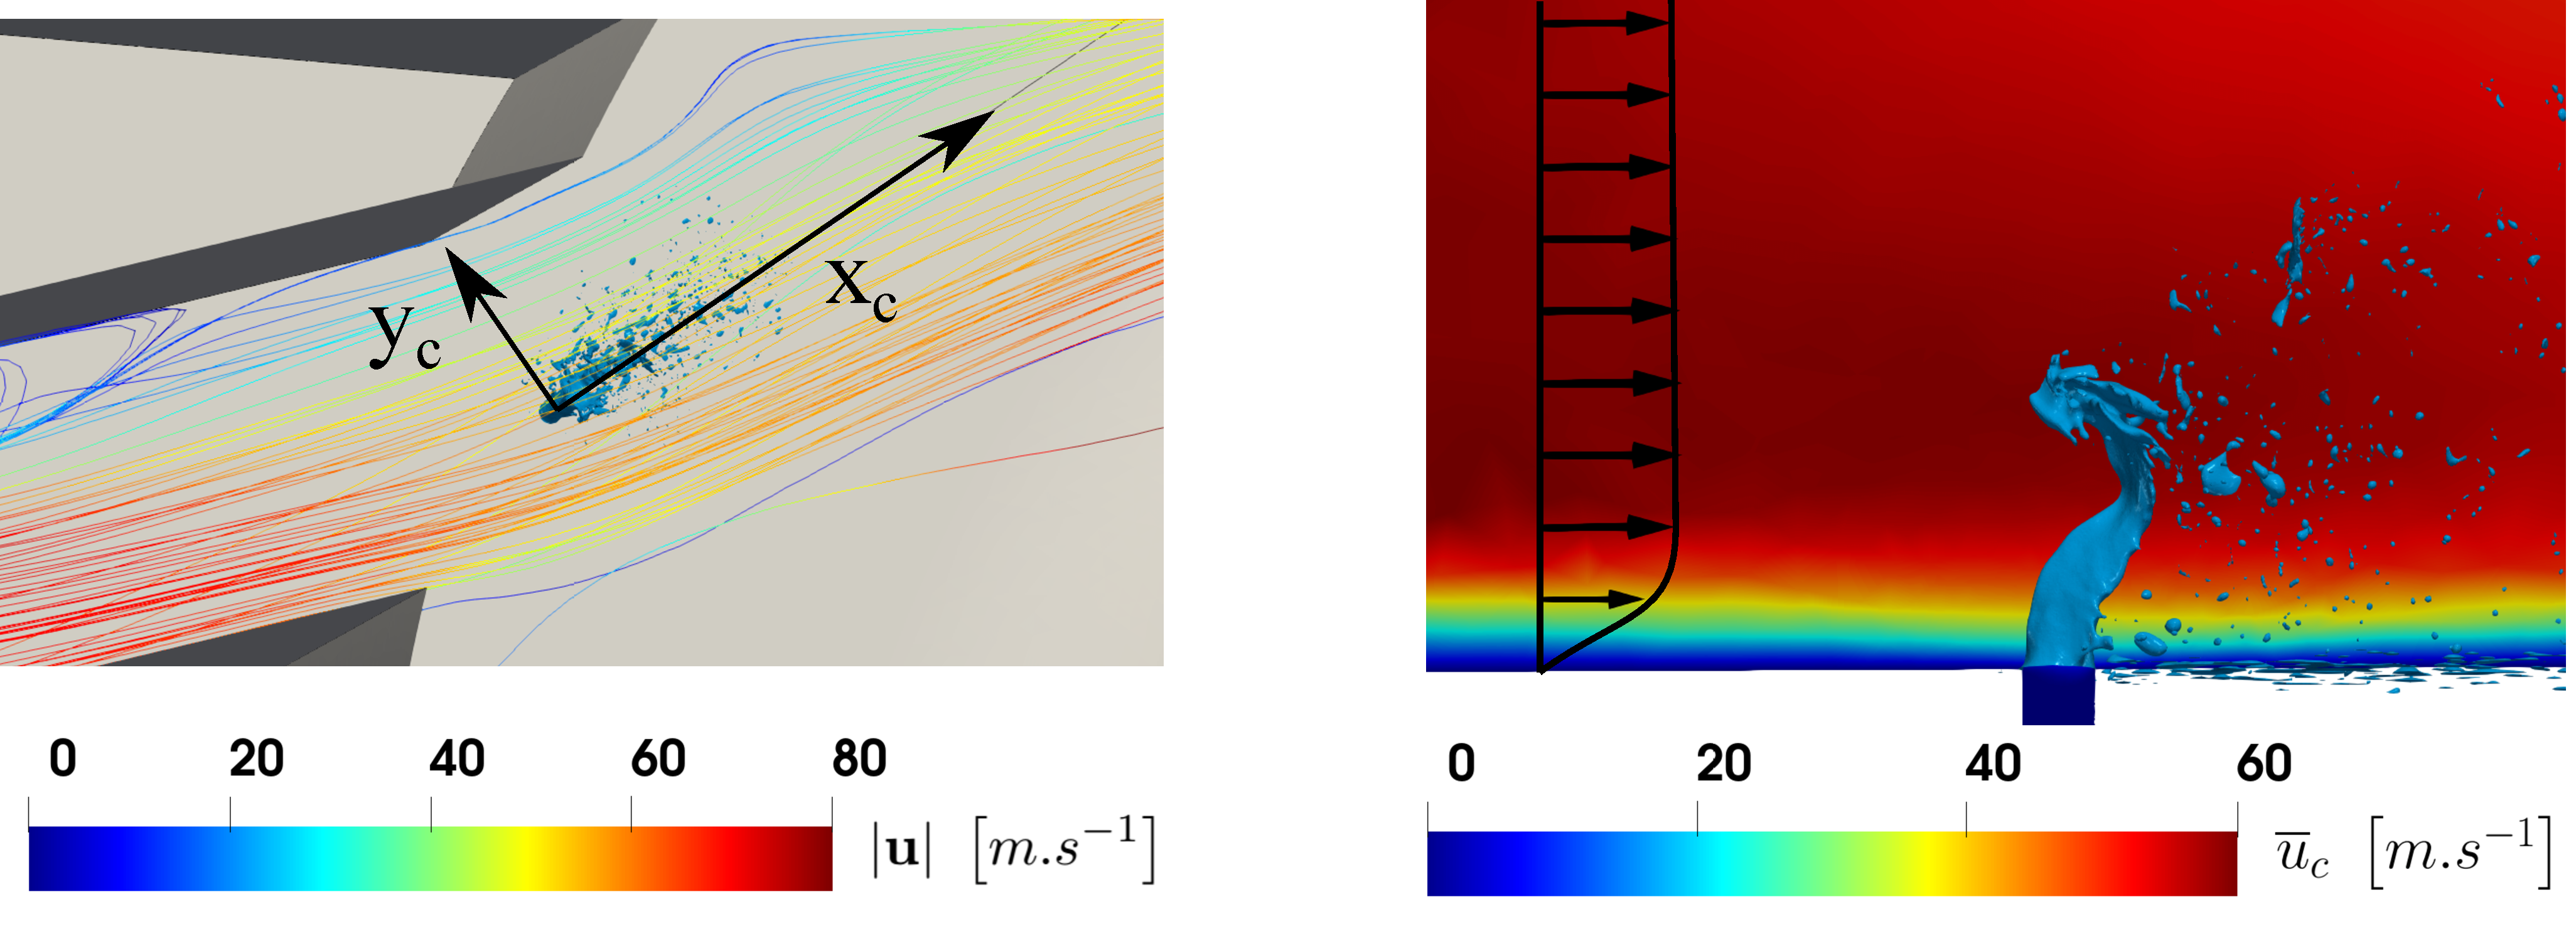
\includegraphics[scale=0.225]{./part3_applications/figures_ch8_resolved/gaseous_profile_streamlines_and_vector}
\caption[Gaseous state at the vicinity of the liquid injection location]{Gaseous state at the vicinity of the liquid injection location. \textsl{Left}: gas streamlines through the inlet multipoint vane.  \textsl{Right}: Instaneous BIMER view with mean axial velocity field in plane $y_c = 0$. The mean field corresponds to the gaseous solution without liquid used as an inlet condition, the jet has been added for comparison. The vectors represent the velocity profile just upstream the injector. The velocity profile has been displaced upstream in the picture for a better visualization.}
% OJO: ficheros generados para el perfil de velocidades estan en Ongoing\ICS_study\u_mean_profiles\cases_probes\mesh_refined_DX0p5_ics_no_actuator_flat_BL_with_turbulence_L3p00_up2p7
\label{fig:BIMER_Umean_profile_with_jet}
\end{figure}



\begin{figure}[ht]
\centering
	\centering
   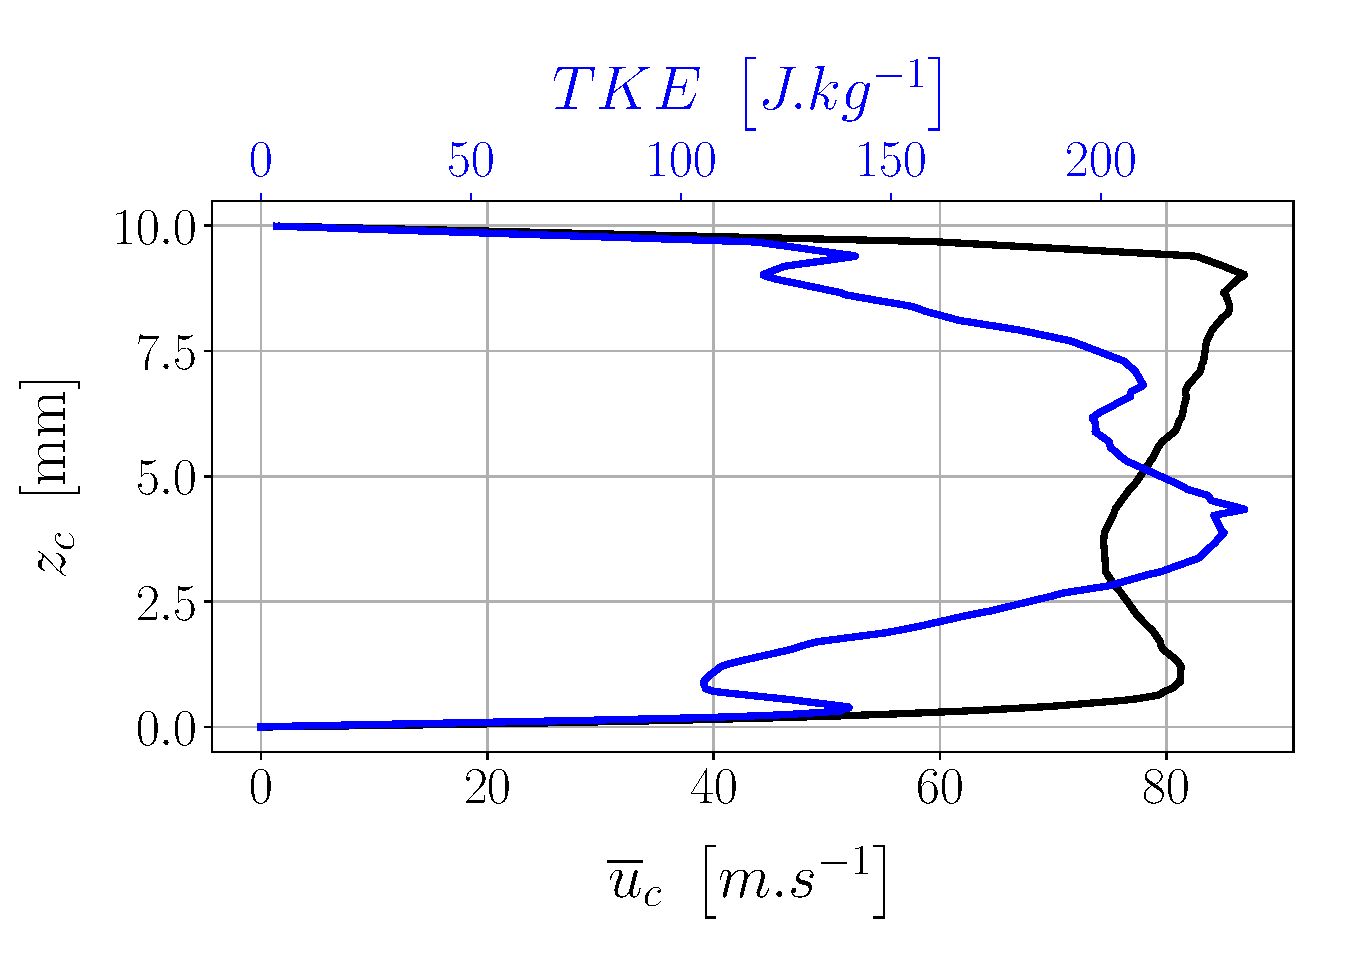
\includegraphics[scale=0.4]{./part3_applications/figures_ch8_resolved/gas_inlet_profiles}
   \vspace*{-0.15in}
   \caption{Profiles of $\overline{u}_c$ and $TKE$ along the vertical line right upstream the liquid injector}
\label{fig:BIMER_gas_inlet_profiles}
\end{figure}




\subsubsection*{Liquid phase}

In the operating point studied, the total liquid mass flow rate injected is $\dot{m}_{l,\mathrm{total}} = 1.64$ g s$^{-1}$. The staging parameter, defined in Eq. (\ref{eq:BIMER_staging_parameter}), is $\alpha = 15 ~\%$, meaning that amount of liquid goes through the pilot stage and $85 ~\%$ of fuel goes through the take-off. Therefore, $\dot{m}_{l,\mathrm{pilot}} = 0.25$ g s$^{-1}$ and $\dot{m}_{l,\mathrm{takeoff}} = 1.39$ g s$^{-1}$. This quantity of fuel is injected through 10 injection holes that conform the take-off stage; assuming that fuel repartition is done equally through all the channels, each injector introduces $0.139$ g s$^{-1}$ of dodecane fuel, which is equivalent to a flow rate of $Q_l = 185.3$  mm$^3$ s$^{-1}$ given the dodecane density from Table \ref{tab:dodecane_properties}. From this flow rate, the bulk liquid velocity $u_l$ can be estimated knowing an injection diameter of $d_\mathrm{inj} = 0.3$ mm:

\begin{equation}
u_l = \frac{Q_l}{\pi d_\mathrm{inj}^2 / 4} = 2.6 ~ \mathrm{m}.\mathrm{s}^{-1}
\end{equation}


The velocity profile imposed at the liquid inlet shown in Figure \ref{fig:BIMER_liquid_injector_views} is a Poiseuille profile with the mean velocity of value $u_l$. With the estimate values for bulk liquid and gaseous velocities, the liquid properties given in Table \ref{tab:dodecane_properties} and the gaseous properties from Table \ref{tab:gaseous_operating_points_BIMER}, the momentum flux ratio $q$ and the Weber number based on the gaseous phase $We_g$ can now be calculated:

%\begin{subequations}
%\begin{align}
%q &=  \frac{\rho_l u_l^2}{\rho_g u_g^2} \approx 4 \\
%We_g &=  \frac{\rho_g d_{inj} u_g^2}{\sigma} \approx 14
%\end{align}
%\end{subequations}

\begin{equation}
q =  \frac{\rho_l u_l^2}{\rho_g u_g^2} \approx 2 ~~~~ ; ~~~~  We_g =  \frac{\rho_g d_\mathrm{inj} u_g^2}{\sigma} \approx 30
\end{equation}

%\begin{subequations}
%\begin{align}
%q &=  \frac{\rho_l u_l^2}{\rho_g u_g^2} = \frac{750 \cdot 2.6^2}{0.816382 \cdot 38.05^2} = 4 \\
%We_g &=  \frac{\rho_g d_{inj} u_g^2}{\sigma} = \frac{0.816382 \cdot 0.3 mm \cdot 38.05^2}{25.35 10^{-3}} \approx 14
%\end{align}
%\end{subequations}

Figure \ref{fig:location_BIMER_op_in_breakup_map} shows the BIMER JICF operating point classified in the breakup diagram of \citeColor[wu_breakup_1997], which is located in the multimode breakup regime. The governing parameters characterizing the BIMER operating point are summarized in Table \ref{tab:bimer_sps_operating_point}. The dimensionless numbers from Eqs. (\ref{eq:dimensionless_numbers_jicf}) are also calculated. Two simulations have been performed with three different element resolutions at the liquid-gas interface $\Delta x_\mathrm{min} = 15, 10~\mu$m, the nomenclature for each case is given in Table \ref{tab:BIMER_resolved_simulations_performed}.

\begin{figure}[ht]
     \centering
     \includeinkscape[inkscapelatex=false,scale=0.6]{./part3_applications/figures_ch8_resolved/BIMER_breakup_regime_our_operating_point}
     \vspace*{-0.1in}
     \caption{Location of simulated operating condition in the breakup map by \citeColor[wu_breakup_1997]}
	% See: https://stackoverflow.com/questions/35210337/can-i-plot-several-histograms-in-3d/35225919
      \label{fig:location_BIMER_op_in_breakup_map}
\end{figure}

\begin{table}[!h]
\centering
\caption{BIMER operating point to perform resolved atomization simulations}
\begin{tabular}{lccc}
\thickhline
\textbf{Parameter} & \textbf{Symbol} & \textbf{Units} &  \textbf{Value} \\
\thickhline
Nozzle diameter & $d_\mathrm{inj}$ & mm & 0.3 \\
%\hline
Gas bulk velocity & $u_g$ & m s$^{-1}$ & 56 \\
%\hline
Gas flow rate & $Q_g$ & m$^3$ s$^{-1}$ & $2.2833 \cdot 10^{-3}$   \\
%\hline
Liquid bulk velocity & $u_l$ & m s$^{-1}$ & 2.6  \\
%\hline
Liquid flow rate & $Q_l$ & mm$^3$ s$^{-1}$ & 185.3  \\
%\hline
Ambient pressure & $p_\mathrm{amb}$ & bar &  1 \\
%\hline
Gas temperature & $T_g$ & K & 433 \\
%\hline
Liquid temperature & $T_l$ & K & 293 \\
%\hline
Gas density & $\rho_g$ & kg m$^{-3}$ & 0.82 \\
%\hline
Liquid density & $\rho_l$ & kg m$^{-3}$ & 750 \\
%\hline
Gas viscosity & $\mu_g$ & kg m$^{-1}$ s$^{-1}$ & $2.39 \cdot 10^{-5}$ \\
%\hline
Liquid viscosity & $\mu_l$ & kg m$^{-1}$ s$^{-1}$ &  $1.36 \cdot 10^{-3}$ \\
%\hline
Surface tension & $\sigma$ & kg s$^{-2}$ &  0.025  \\
\thickhline
Gas Reynolds number & $Re_g$ & - & $20 \cdot 10^3$ \\ %& $9.80 \cdot 10^3$ \\
%\hline
Liquid Reynolds number & $Re_l$ & - & 430 \\
%\hline
Momentum ratio & $q$ & - & 2 \\ %4  \\
%\hline
Gas Weber number & $We_g$ & - & 30 \\ %14 \\
%\hline
Liquid Weber number & $We_l$ & - & 60 \\
%\hline
Relative Weber number & $We_\mathrm{rel}$ & - & 52 \\ %12 \\
%\hline
Aerodynamic Weber number & $We_\mathrm{aero}$ & - & 0.067 \\
%\hline
Ohnesorge number & $Oh $ & - & 0.018 \\
%\hline
Density ratio & $r$ & - & 915 \\
%\hline
\thickhline
\end{tabular}
\label{tab:bimer_sps_operating_point}
\end{table}

\begin{table}[!h]
\centering
\caption{Nomenclature for resolved atomization simulations}
\begin{tabular}{cc}
\thickhline
%$\pmb{\Delta} x_\mathrm{min}$ [$\pmb{\mu}$$\textbf{m}])  &  \multicolumn{2}{c}{\textbf{Operating condition}} \\ 
$\Delta x_\mathrm{min}$ [$\mu$m]  &  Denomination \\ 
\thickhline
%7.5 & BIMER\_DX07 \\
10 & BIMER\_DX10 \\
15 & BIMER\_DX15 \\
\thickhline
\end{tabular}
\label{tab:BIMER_resolved_simulations_performed}
\end{table}




\section{Definition of liquid characteristic times}

Characteristic times can be defined for the liquid phase in BIMER in the same way it was done for the DLR JICF test case from Chapter \ref{ch5:jicf_resolved_simulations}. Details on the timescales chosen and on their calculation are given in $\S$\ref{sec:ch5_liquid_characteristic_times}. Here, the definitions summarized in Table \ref{tab:jicf_characteristic times} are directly applied to the BIMER test case. The results are shown in Table \ref{tab:BIMER_SPS_characteristic times}. 

\begin{table}[!h]
\centering
\caption{Characteristic physical timescales [$\mu$s] in BIMER simulations}
\begin{tabular}{ccc}
\thickhline
\textbf{Time scale} & \textbf{Expression} & \textbf{BIMER} \\
\thickhline
Inertia & $\tau_\mathrm{in} = \frac{d_\mathrm{inj}}{u_l}$ & 115.38 \\
Aerodynamic breakup  &  $\tau_\mathrm{ab} =  \frac{d_\mathrm{inj}}{u_g - u_l} \sqrt{\frac{\rho_l}{\rho_g}} $ & 256.30 \\
Non-aerodynamic breakup  &  $\tau_\mathrm{nb} = \frac{d_\mathrm{inj}}{u_l} We_l^{1/3} $ &  453.81 \\
Capillary & $\tau_\mathrm{cap} = \sqrt{\frac{\rho_l d_\mathrm{inj}^3}{8 \sigma}}$ & 318.20 \\
\thickhline
\end{tabular}
\label{tab:BIMER_SPS_characteristic times}
\end{table} 

As shown in the previous table, the lower timescale is found for the inertia processes and hence those are governing breakup. Yet, all timescales are of the same order of magnitude, as opposed to the timescales of the DLR JICF summarized in Figure \ref{tab:jicf_characteristic times} where the fastest timescale (inertia) was around $100$ times smaller than the slowest (capillary). For the BIMER operating point studied, the inertia timescale is only $3$ times smaller than the capillary one, which is not even the slowest (in this case, it corresponds to the non-aerodynamic breakup timescale). The fact that the timescales in this case are closer to each other agree with the location of the BIMER operating point in the breakup diagram of Figure \ref{fig:location_BIMER_op_in_breakup_map} \citepColor[pilch_use_1987]. Besides the physical timescales, the droplets arrival times to the sampling planes depicted in Figure \ref{fig:BIMER_local_FoR_and_sampling_planes}. These ones are summarized in Table \ref{tab:BIMER_SPS_characteristic_droplet_sampling_times}. 


%\begin{table}[!h]
%\centering
%\caption{Characteristic droplet arrival times to sampling planes $\tau_\mathrm{dr_{x_c}}$ [$\mu$s] in BIMER simulations}
%\begin{tabular}{ccccccc}
%\thickhline
%\textbf{Case} & $x_c/d_\mathrm{inj} = 3.33$ & $x_c/d_\mathrm{inj} = 5$ & $x_c/d_\mathrm{inj} = 6.67$ & $x_c/d_\mathrm{inj} = 8.33$ & $x_c/d_\mathrm{inj} = 10$ & $x_c/d_\mathrm{inj} = 11.66$  \\
%\thickhline 
%BIMER\_DX07 & 321 & 340 & 359 & 395 & 434 & 589 \\
%BIMER\_DX10 & 310 & 331 & 354 & 387 & 428 & 585 \\
%BIMER\_DX15 & 450 & 511 & 562 & 569 & 633 & 729 \\
%\thickhline
%% NOTA: valores DX07 corresponden en realidad a dx_min = 5 µm
%% NOTA: valores DX07 a partir de 8.33 han sido estimados a ojo
%\end{tabular}
%\label{tab:BIMER_SPS_characteristic_droplet_sampling_times}
%\end{table}


%\begin{table}[!h]
%\centering
%\caption{Characteristic droplet arrival times to sampling planes $\tau_\mathrm{dr_{x_c}}$ [$\mu$s] in BIMER simulations}
%\begin{tabular}{cccc}
%\thickhline
%\textbf{Case} &  $x_c/d_\mathrm{inj} = 5$ & $x_c/d_\mathrm{inj} = 6.67$  \\
%\thickhline 
%%BIMER\_DX07 & 340 & 359 \\
%BIMER\_DX10 & 331 & 354 \\
%BIMER\_DX15 & 511 & 562 \\
%\thickhline
%% NOTA: valores DX07 corresponden en realidad a dx_min = 5 µm
%% NOTA: valores DX07 a partir de 8.33 han sido estimados a ojo
%\end{tabular}
%\label{tab:BIMER_SPS_characteristic_droplet_sampling_times}
%\end{table}


\begin{table}[!h]
\centering
\caption{Characteristic droplet arrival times to sampling planes $\tau_\mathrm{dr_{x_c}}$ [$\mu$s] in BIMER simulations}
\begin{tabular}{cccccc}
\thickhline
\textbf{Case} &  $x_c = 1.5~\mathrm{mm}$ & $x_c = 2 ~ \mathrm{mm}$ & $x_c = 2.5 ~ \mathrm{mm}$ & $x_c = 3 ~ \mathrm{mm}$ \\
\thickhline 
%BIMER\_DX07 & 340 & 359 & & \\
BIMER\_DX10 & 331 & 354 & 380 & 398 \\
BIMER\_DX15 & 511 & 562 & 569 & 582 \\
\thickhline
% NOTA: valores DX07 corresponden en realidad a dx_min = 5 µm
% NOTA: valores DX07 a partir de 8.33 han sido estimados a ojo
\end{tabular}
\label{tab:BIMER_SPS_characteristic_droplet_sampling_times}
\end{table}


\section{Jet evolution}
\label{sec:ch8_BIMER_jet_evolution}

The jet evolution at the early instants of the injection process is shown in Figure \ref{fig:BIMER_jet_establishment}. Snapshots are shown for values of dimensionless time $t^*$ defined by Eq. (\ref{eq:t_dimensionless_with_tau_in}), in which the physical time is expressed in relation to the timescale $\tau_\mathrm{in}$ from Table \ref{tab:BIMER_SPS_characteristic times}. As in the simulations from Chapter \ref{ch5:jicf_resolved_simulations}, this timescale has been chosen since is the same for all simulations and the jets depicted represent therefore equivalent instants.

Images show the features of a liquid JICF configuration: the jet leaves the injection nozzle and enters into contact with the crossflow, which has the effect of deforming the liquid column and deviating the jet towards the crossflow direction (which is represented in Figure \ref{fig:BIMER_jet_establishment} by the black solid line). However, the jet topology is very different to a classical JICF configuration such as the one studied in Chapter \ref{ch5:jicf_resolved_simulations}: both surface and column breakup are present (more details are given on the next section), but in BIMER column breakup creates mainly thin liquid sheets that are quickly disintegrated into small droplets (more details are given on the next section). The jet does not penetrate far and the deviation of the jet column towards the crossflow direction is not highly significant, since breakup occurs close to the injection location (as demonstrated in $\S$\ref{ch8:sec_BIMER_DC_characterization}). The low penetration is due to the low value of $q$ for this operating point, which is the parameter governing the jet penetration. The quick disintegration to low droplets and the instabilities shown along the liquid columns, which are clearly different to the column waves analyzed in $\S$\ref{subsec:ch5_instabilities_presence} for the classical JICF configuration), are attributed to the highly turbulent state of the flow, as shown by the $TKE$ profile in Figure \ref{fig:BIMER_gas_inlet_profiles}. The interface resolution has also an effect on the jet topology: the coarse case (DX15) penetrates further than the fine one (DX10) and undergoes more deviation due to the action of the crossflow. 



%\label{ch8:resolved_atomization_simulations}

%\begin{table}[!h]
%\centering
%\caption{Operating point}
%\begin{tabular}{cccc}
%\thickhline
%$u_g$ [m s$^{-1}$] &  38 \\
%\hline
%$u_l$ [m s$^{-1}$] &  2.6 \\
%\hline
%\hline
%$q$ & 4 \\ %4.3 \\
%\hline
%$We_g$ & 14 \\
%\hline
%\end{tabular}
%\label{tab:bimer_sps_operating_point}
%\end{table}
%
%\begin{table}[!h]
%\centering
%\caption{Operating point}
%\begin{tabular}{cccc}
%\thickhline
%$u_g$ [m s$^{-1}$] &  $u_l$ [m s$^{-1}$] & $q$ &  $We_g$  \\
%\hline
%38 &  2.6 & 4 & 15 \\
%\thickhline
%\end{tabular}
%\label{tab:bimer_sps_operating_point}
%\end{table}



%\begin{figure}[h!]	
%	\centering
%	\includeinkscape[inkscapelatex=false,scale=0.75]{./part1_numerical_approaches/figures_ch3/gas_injection_area_multipoint}
%	\caption{Area to calculate bulk gas velocity}
%	\label{fig:gas_injection_area_multipoint}
%\end{figure}


%According to \textbf{2016 Eckel}, the velocity is not the gaseous one but the relative:
%
%\begin{equation}
%\tau_c = \sqrt{\frac{\rho_l}{\rho_g}} \frac{d_\mathrm{inj}}{u_\mathrm{rel}} = \sqrt{\frac{750}{0.816382 }} \frac{0.3 ~mm}{38 - 2.6} = 0.26
%\end{equation}
%
%which is actually very similar.



%\subsection{Breakup topology}

%The topology is super different with respecto to DLR JICF!! 


\subsection{Breakup topology}
\label{ch8:subsec_BIMER_breakup_topology}

Classification of the BIMER operating point considered in the breakup map of Figure \ref{fig:location_BIMER_op_in_breakup_map} estimates the regime to be comprised in the column breakup region, within the multimode breakup regime but very close to bag breakup. This regime is characterized by a mixture of breakup properties from both bag breakup, like enough spacing among column instabilities so that both bags and ligaments can be formed and lead to breakup, and shear breakup, such as surface stripping \citepColor[sallam_breakup_2004]. As in any traditional JICF, these are also expressed in terms of column and surface breakup features. Figure \ref{fig:BIMER_breakup_topology} shows these two phenomena observed in BIMER. In the first snapshot of the column breakup series, the red circle denotes the onset of an instability which propagates along the jet vertical and lateral directions. The vertical-propagating instability evolves into a thin sheet (green highlight) that eventually breaks into large liquid ligaments during primary atomization: this is the column breakup phenomenon. As in a classical JICF, these ligaments will propagate further downstream and keep on breaking. This sheet is followed by a column flattening in the lateral directions that is not typical from a classical JICF configuration (black highlight) and which modifies the ligaments produced later through column breakup. After this flattening, the process repeats again from the beginning. The lateral-propagating instabilities evolve in the surface breakup phenomenon, as illustrated in the bottom snapshots of Figure \ref{fig:location_BIMER_op_in_breakup_map}. As in the surface breakup of the canonical JICF depicted in Figure \ref{fig:jicf_surface_breakup_ug75_dx10}, two different features are highlighted: the generation of very small droplets (green highlight), whose size is of the order of the mesh resolution and will eventually disappear producing mass losses in the simulations, and the generation of small ligaments (red highlight) which break faster into smaller droplets that are later transported. Both column and surface breakup phenomena have been widely observed in traditional JICF configurations and are also captured in BIMER. What has been unexpected, though, is the onset of both phenomena through a central instability that evolves along the column vertical and sides direction, as well as the column flattening in the lateral direction. Both phenomena have been observed in both resolutions simulated and might be associated to the gaseous swirl. Nevertheless, no analysis on the breakup phenomena in liquid JICF with swirl (either in the gas or liquid phases) have been reported in literature to the knowledge of the authors.%, even though some analysis on swirled JICF are available on other magnitudes (\textbf{ref:XX?}).

\begin{figure}[ht]
\centering
\includegraphics[scale=0.125]{./part3_applications/figures_ch8_resolved/breakup_topology/DX10_breakup_both}
\caption{Breakup in BIMER, case DX10. }
% Soluciones:
% column breakup: sol02_37, sol03_08,_20,_32, sol04_07,_19
% surface breakup:sol03_32,37, sol04_05,10,13
\label{fig:BIMER_breakup_topology}
\end{figure}

\subsection{Jet establishment}

Esbalishment of the liquid jet in the BIMER configuration is monitored by quantifying the evolution of the number of mesh elements and the liquid volume inside the domain calculated from Eq. (\ref{eq:liquid_volume_from_levelset_definition}). Time has been non-dimensionalized with the timescale $\tau_{\mathrm{dr}_{x_c/=3}}$ as given in Table \ref{tab:BIMER_SPS_characteristic_droplet_sampling_times}:

%\begin{equation}
%\label{eq:t_prime_BIMER_with_tau_drx10}
%t^{\prime} = \frac{t}{\tau_{\mathrm{dr}_{x_c/d_\mathrm{inj}=10}}}
%\end{equation}

%\begin{equation}
%\label{eq:t_prime_BIMER_with_tau_drx10}
%t^{\prime} = t / \tau_{\mathrm{dr}_{x_c/d_\mathrm{inj}=6.67}}
%\end{equation}

\begin{equation}
\label{eq:t_prime_BIMER_with_tau_drx10}
t^{\prime} = t / \tau_{\mathrm{dr}_{x_c/=3}}
\end{equation}


Results are shown in Figure \ref{fig:BIMER_volume_nelem_evolution}. Volume increase linearly at the early instants of injection due to the constant flow rate injected. At a certain point, the slope of $V_l$ starts to decrease due to droplets being removed from the simulation when reaching the sponge layer. Liquid volume shows establishment at value between $V_l = 0.75$ and $0.8$ mm$^3$. The evolution of the number of elements in the simulation shows a fast establishment for $DX15$ at a value around $60 \cdot 10^6$ elements. Case DX10 shows maximum values around $100 \cdot 10^6$ elements, and shows large magnitude oscillations due to the clusters of droplets resulting from column breakup and reaching the sponge layer at the same time instants, causing large decreases in the number of elements and small ones in the liquid volume evolution. The decreases in the number of elements are specially notorious for case DX10, which shows an abrupt decrease at the end of the simulation time from $125 \cdot 10^6$ to $90 \cdot 10^6$ elements. The time among element peaks might be associated to the frequencies of column breakup sheets/ligament shedding observed in Figure \ref{fig:BIMER_breakup_topology}. Further assessing this hypothesis would need the simulations to run for longer, since these frequencies associated to column breakup are low (which are low when compared to the frequencies of droplets ejected from surface breakup) and larger simulation times would be needed. This has not done in this work due to constraints in computational resources and since the actual purpose of these simulations is the obtention of data for creating converged SLIs, which has been achieved with the physical times simulated (see $\S$\ref{sec:ch8_learning_SLI_in_BIMER})

\clearpage

\begin{figure}[ht]
\centering
\includeinkscape[inkscapelatex=false,scale=0.8]{./part3_applications/figures_ch8_resolved/jet_establishment}
\caption{Establishment of BIMER resolved atomization simulations at several time instants}
\label{fig:BIMER_jet_establishment}
\end{figure}

\clearpage







\begin{figure}[ht]
\centering
\begin{subfigure}[b]{0.45\textwidth}
	\centering
   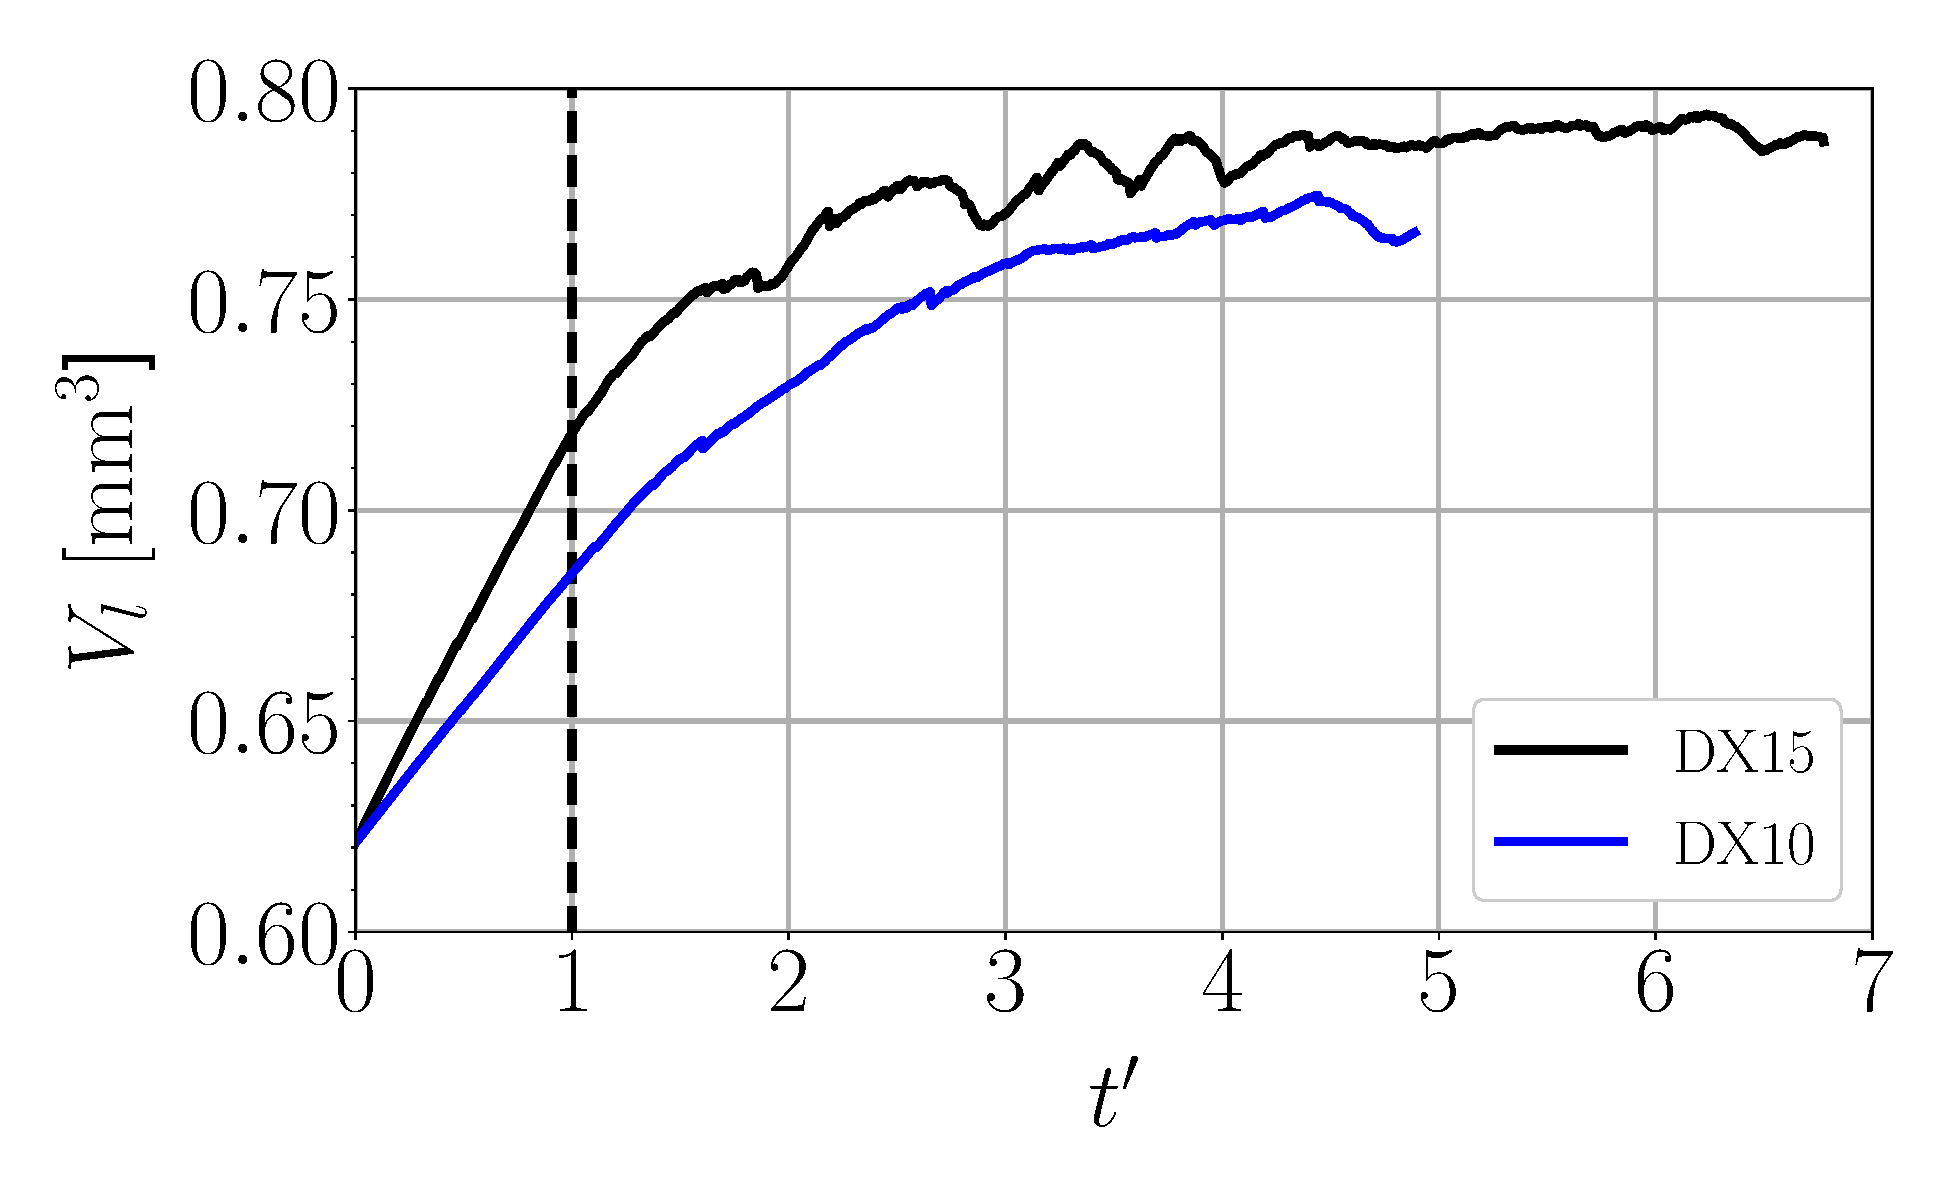
\includegraphics[scale=0.24]{./part3_applications/figures_ch8_resolved/BIMER_liquid_volume_increase}
   \vspace*{-0.25in}
   %\caption{Liquid volume}
   \label{fig:BIMER_liquid_volume_evolution} 
\end{subfigure}
\hfill
\begin{subfigure}[b]{0.45\textwidth}
	\centering
   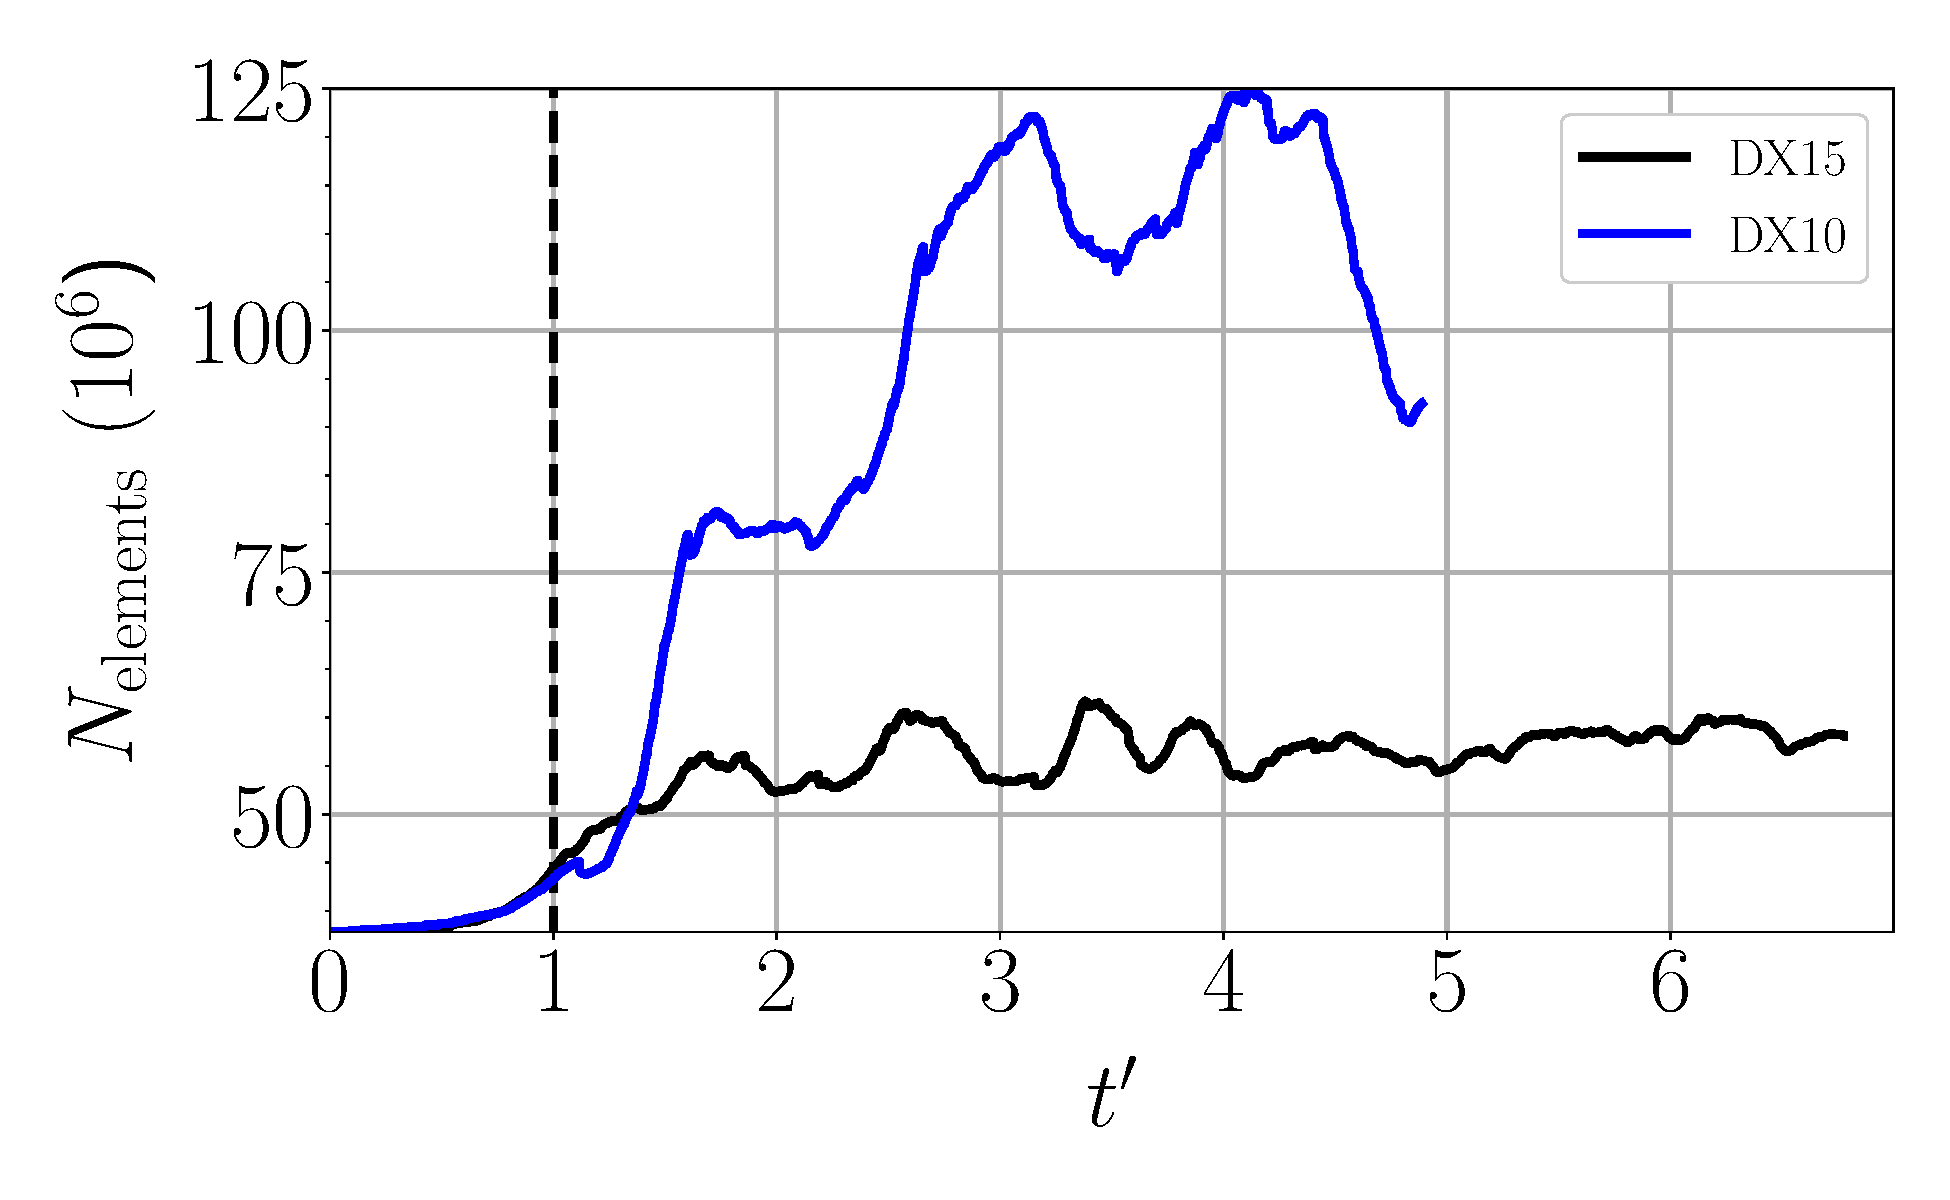
\includegraphics[scale=0.24]{./part3_applications/figures_ch8_resolved/BIMER_nelem_increase}
   \vspace*{-0.25in}
   %\caption{Zoomed-in view of Figure \ref{fig:JICF_nelem_increase_all_t} in range $t^{\prime} \in [0, 2]$}
   \label{fig:BIMER_nelem_increase}
\end{subfigure}
   \caption[Evolution of liquid volume (\textsl{left}) and number of mesh elements (\textsl{right}) with time in BIMER resolved simulations]{Evolution of number of mesh elements (\textsl{left}) and number of mesh elements (\textsl{right}) with time in BIMER resolved simulations. The dashed, black vertical line corresponds to $t^\prime = 1$, time instant when the first droplet reaches the sampling plane $x_c/d_\mathrm{inj} = 10$}
\label{fig:BIMER_volume_nelem_evolution}
\end{figure}



\section{Jet trajectories}

Vertical trajectories for quantifying the penetration of BIMER can be obtained by applying the methodologies described in $\S$\ref{sec:ch5_tools_jicf_trajectories}. The maximum gradient method of the mean levelset function is used. The trajectories obtained are shown in Figure \ref{fig:BIMER_trajectories}. There are no experimental data to compare the BIMER resolved simulations: yet, the trajectory given by Eq. (\ref{eq:jicf_trajectory_becker}) with $q = 2$, from the study by \citepColor[becker_breakup_2002], is used for comparison. This expression was chosen since it was the only one found in literature (see Table \ref{tab:correlations_experimental_JICF} for a compilation of several correlations) valid at low $q$ values. The actual comparison with experiments show a good match among the correlation and the experiments closer to injector: numerical trajectories are within the bounds and show a similar deviation trend to the experiments for $x_c/d_\mathrm{inj} < 3$ in case DX15 and $x_c/d_\mathrm{inj} < 2$ in case DX15, where curves also display a smooth evolution. This confirms again the ability of the ACLS methodology to capture JICF physical features. After the indicated values, however, the numerical trajectories underestimate the experimental correlation and show a peaky behaviour: the jet has undergone atomization and the jet is in dispersed-phase. Case DX15 shows still a smooth curve until further downstream, while DX10 shows a peakier behaviour which is due to a faster disintegration of the jet (it will be demonstrated in $\S$\ref{subsec:ch8_BIMER_DC_topology} that the obtained dense core lengths are smaller for DX10 than for DX15). The presence of droplets in the dispersed phase region is highly intermitent, which leads to low values of the mean levelset function in this region and to the axial limits in the trajectories found in the figures: no more gradient points are found at $x_c / d_\mathrm{inj}$ for DX15 and at $x_c / d_\mathrm{inj} > 4$ for DX10.


\begin{figure}[ht]
\centering
   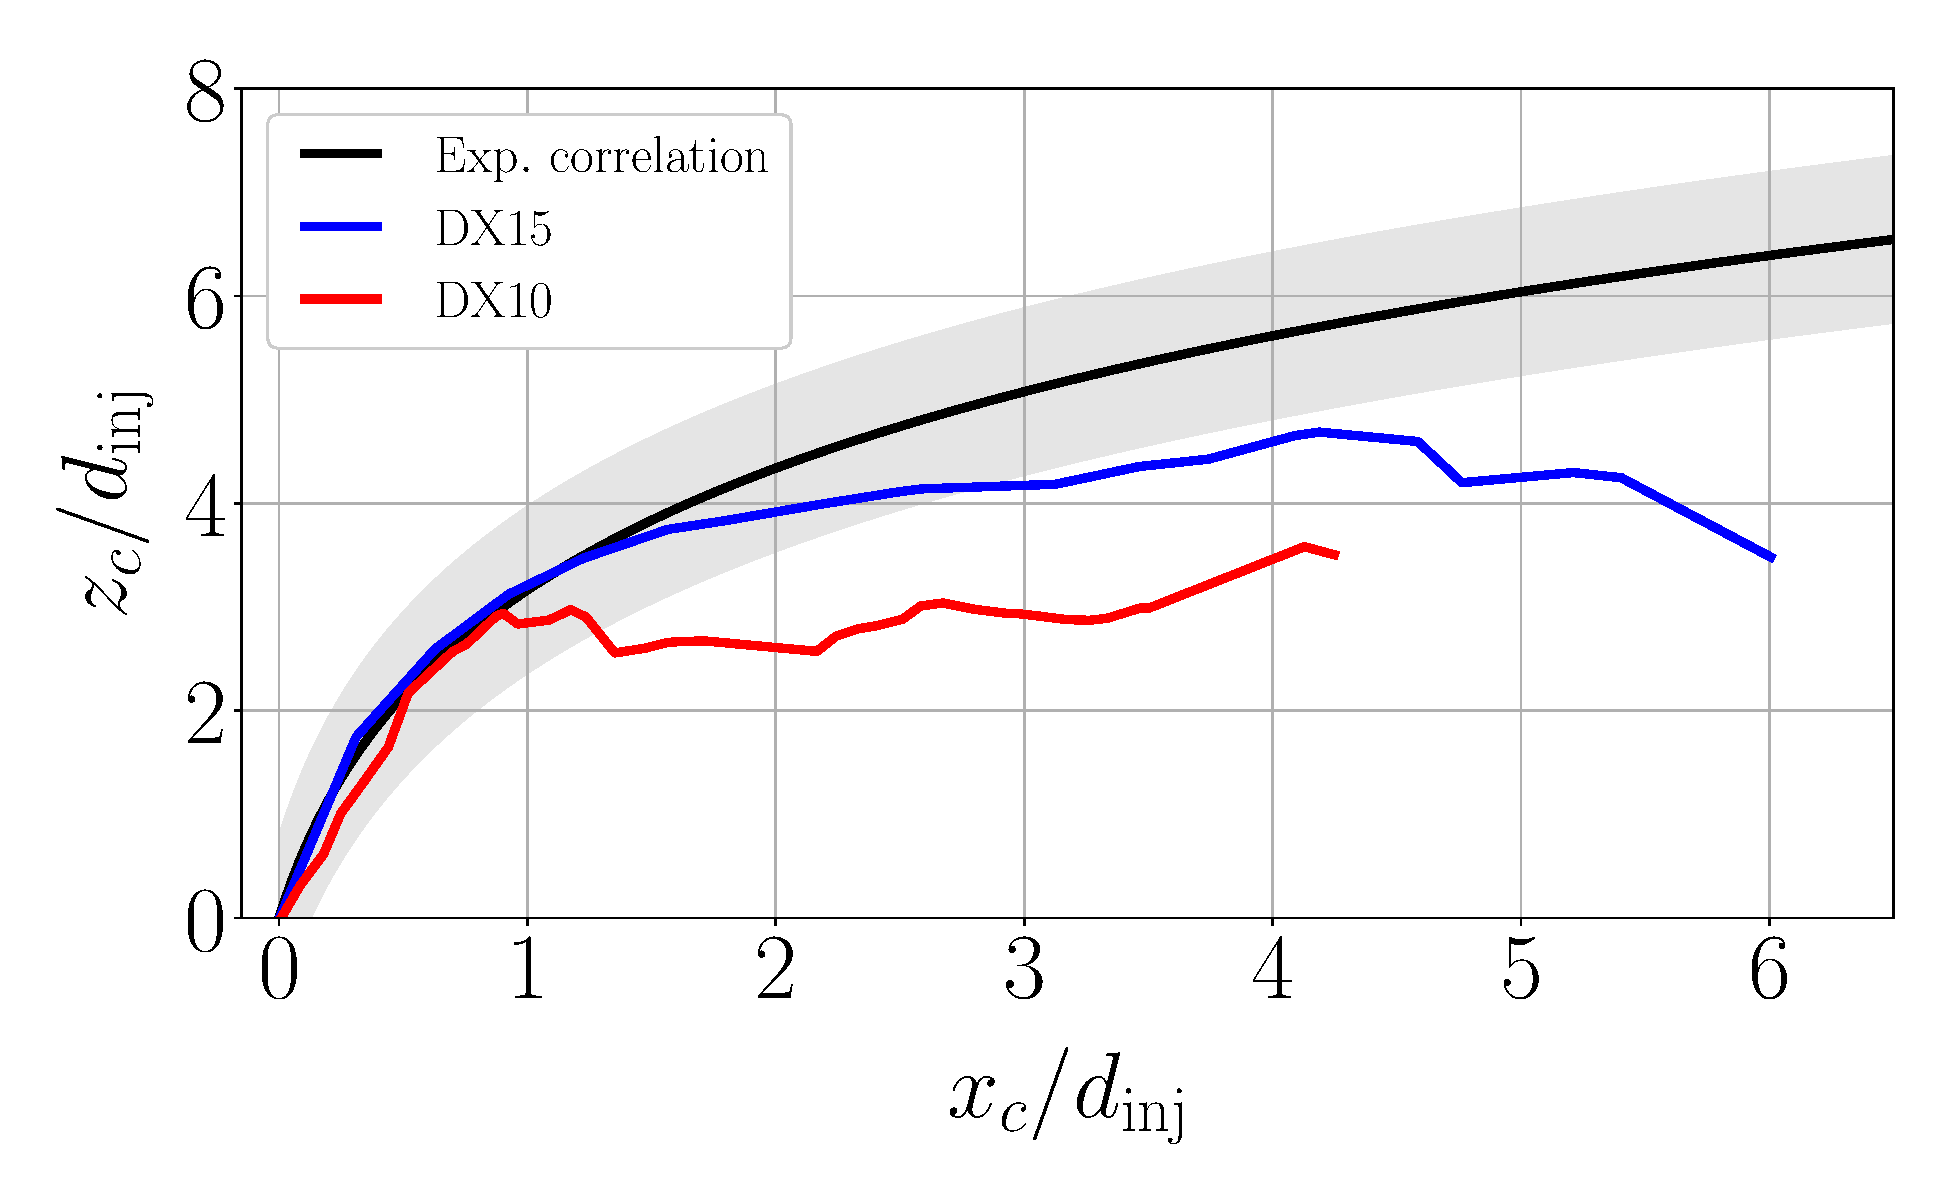
\includegraphics[scale=0.3]{./part3_applications/figures_ch8_resolved/trajectories_BIMER}
   \caption[BIMER trajectories]{BIMER trajectories. The experimental correlation from Eq. (\ref{eq:jicf_trajectory_becker}) \citepColor[becker_breakup_2002] is plotted for comparison}
\label{fig:BIMER_trajectories}
\end{figure}


\section{Perturbation effect ot jet dense core}
\label{ch8:sec_BIMER_DC_characterization}

As in any liquid JICF, the BIMER configuration also creates a perturbation effect from the liquid towards the gaseous phase due to the blockage effect of the liquid column. Figure \ref{fig:BIMER_jet_air_interaction_up_and_skeleton} left shows an instantaneous view of the jet perturbation effect in the plane $y_c = 0$, where the axial velocity fluctuation field $u^\prime_c$ is plotted. Large fluctuations are produced downstream the injection point due to the liquid jet. In the case of BIMER, the asymmetry in the liquid jet when compared to a traditional JICF will also create asymmetric turbulent structures in the gaseous field ($\S$\ref{subsec:ch8_turbulent_structures_BIMER}), which present a challenge to model with ALM. Regarding the dense core topology, the liquid column deforms by the action of the air from a circular cross-section up to very elongated, slender structures which correspond to the cross-section of the liquid sheet prior to breakup. Similarly to traditional JICFs, kidney-shapes cross-sections are also captured in between the injection point and the sheet. A different with respect to classical JICFs is that due to the less pronounced deviation of the jet, detection of the breakup point belonging to liquid structures which are about to shed due to column breakup might lead to axial breakup locations which are upstream the injection location (as depicted in Figure \ref{fig:BIMER_jet_air_interaction_up_and_skeleton}).



\begin{figure}[ht]
\centering
\includeinkscape[inkscapelatex=false,scale=1.1]{./part3_applications/figures_ch8_resolved/results_dense_core_modeling/jet_air_interaction_up_and_skeleton}
\caption[Interaction between liquid dense core and gaseous phase in BIMER]{Interaction between liquid dense core and gaseous phase in BIMER. \textsl{Left}: Instantaneous $u'_c$ field in a JICF simulation from case DX10. The black contours indicate the lines with zero instantaneous fluctuation $u'_c = 0$, while the white contours denote the location of the interface at the plane. \textsl{Right}: BIMER depicted as a combination of cross-sections in planes $y _c= 0$ and several planes perpendicular to $z_c$ axis.}
\label{fig:BIMER_jet_air_interaction_up_and_skeleton}
\end{figure}

\subsection{Dense core topology characterization}
\label{subsec:ch8_BIMER_DC_topology}

In order to characterize the dense core topology, the methodology detailed in $\S$\ref{subsec:ch5_jet_dense_core_extraction} is applied. As explained, the dense core is represented by its breakup point coordinates $\left( x_b, z_b \right)$ and its width $w$. The temporal evolution of such coordinates for the simulations performed is shown in Figure \ref{fig:BIMER_xb_zb_w_evolution}. All temporal signals display a sawtooth shape as in the case of the classical JICF signals from Figure 
\ref{fig:JICF_xb_zb_w_evolution}, with periodic behaviour of the signals which is associated to the frequencies of ligament stripping. The width signals show a periodic oscillations which in some cases reach a value $w/d_\mathrm{inj} < 1$ (i.e. dense core thinner than the injection diameter), which corresponds to the time instants where the column flattens as shown, for instance, in the snapshots of column breakup in Figure \ref{fig:BIMER_breakup_topology}. The signal $x_b$ from case DX10 displays at some points a value $x_b < 0$, which indicates that the dense core breakup point has been detected upstream the injection location as shown, for instance, in Figure \ref{fig:BIMER_jet_air_interaction_up_and_skeleton}.

\begin{figure}[ht]
\flushleft
\begin{subfigure}[b]{0.45\textwidth}
	\centering
   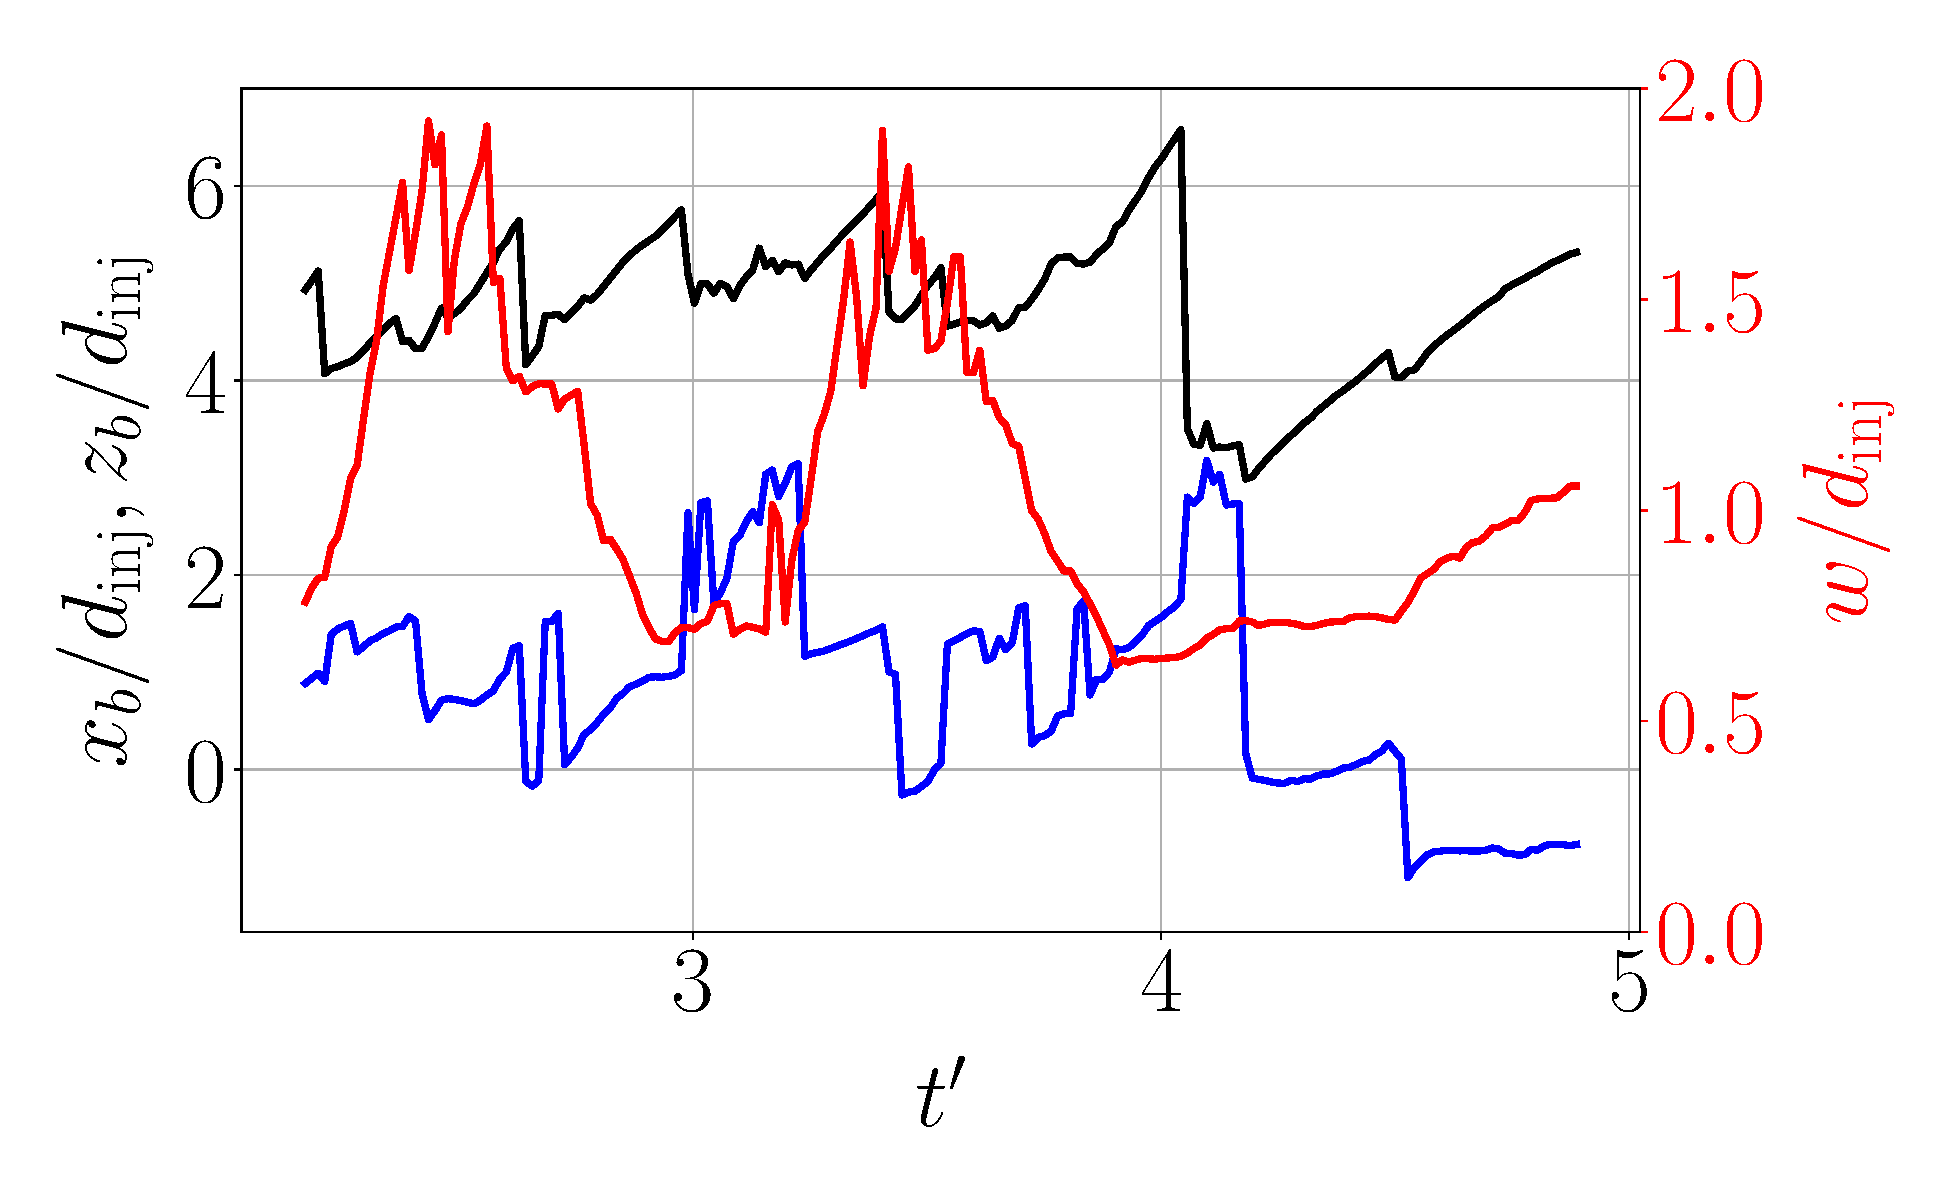
\includegraphics[scale=0.25]{./part3_applications/figures_ch8_resolved/results_dense_core_modeling/instant_xb_zb_w_DX10}
   \vspace*{-0.30in}
   \caption{Case DX10}
   \label{fig:instant_xb_zb_BIMER_w_DX10}
\end{subfigure}
\hfill
\begin{subfigure}[b]{0.45\textwidth}
	\centering
   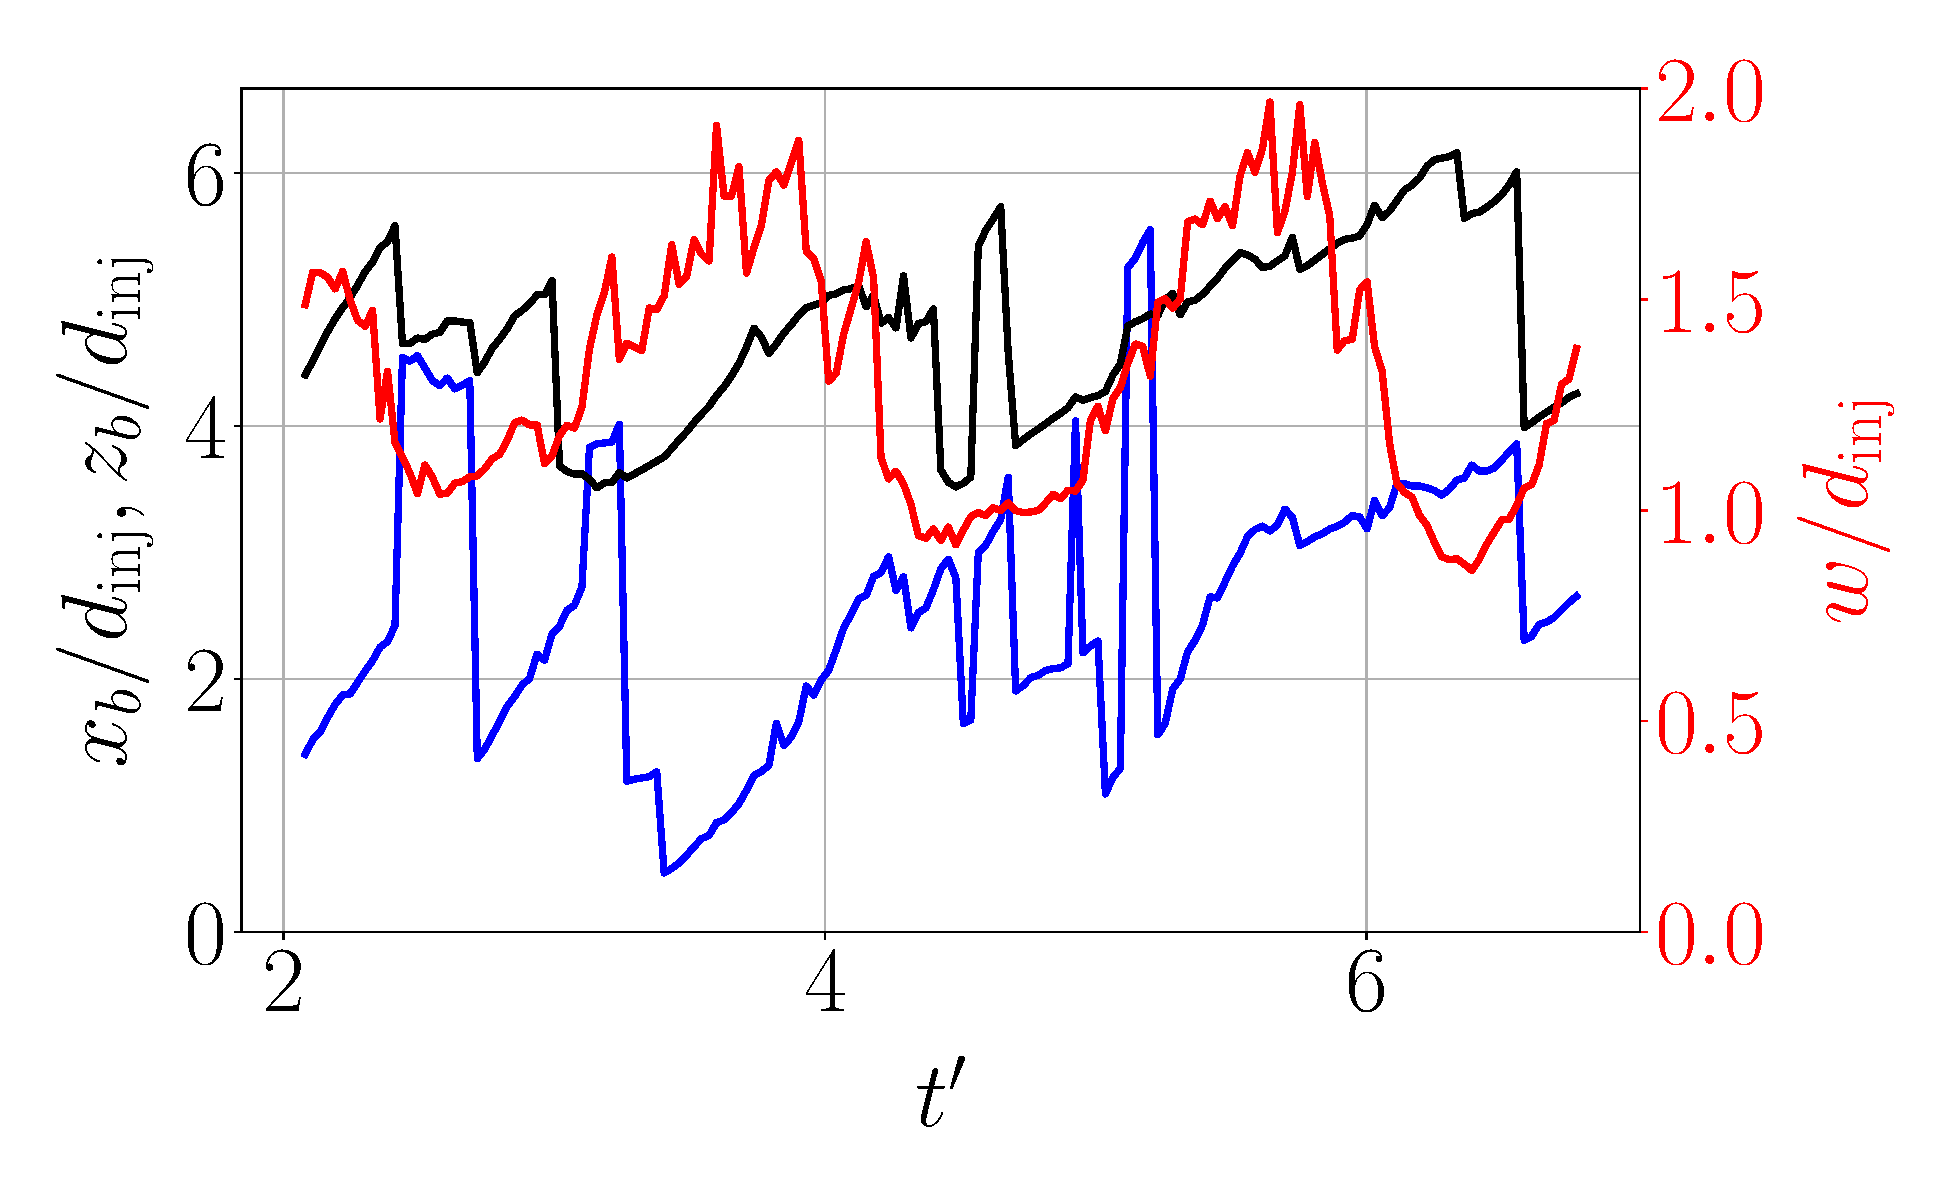
\includegraphics[scale=0.25]{./part3_applications/figures_ch8_resolved/results_dense_core_modeling/instant_xb_zb_w_DX15}
   \vspace*{-0.30in}
   \caption{Case DX15}
   \label{fig:instant_xb_zb_BIMER_w_DX15} 
\end{subfigure}
   \caption{Variation with time of the BIMER dense core breakup point coordinates $x_\mathrm{b}, z_\mathrm{b}$ and width $w$.}
\label{fig:BIMER_xb_zb_w_evolution}
\end{figure}

The evolution of mean quantities for all magnitudes are shown in Figure \ref{fig:BIMER_DC_mean_parameters_convergence}. All cases are shown to be close to convergence. The final mean values are shown in Figure \ref{fig:BIMER_DC_mean_parameters_scatterplots}, where the simulation UG100\_DX10 for the JICF from Chapter \ref{ch5:jicf_resolved_simulations} has been added for comparison. The location of the values in the $\overline{z}_b - \overline{x}_b$ diagram show that $\overline{z}_b > \overline{x}_b$ for both simulations, indicating that the dense core penetrates further vertically than horizontally. There is also a high dependency on resolution: refining the interface cell size does not significantly affect the vertical coordinate $\overline{z}_b$ but reduces considerably the axial breakup location $\overline{x}_b$, reducing hence the dense core length. Similarly, refining the mesh affects the dense core width $\overline{w}$ as shown in Figure \ref{fig:BIMER_DC_mean_parameters_convergence}b.  When comparing with simulation UG100\_DX10, it is seen that both the width and the breakup coordinates are shorter for BIMER. This is coherent with the operating points simulated, since BIMER presents lower values of $q$ and $Re_g$ than the classical JICF which reduces the breakup coordinates and dense core width \citepColor[patil_liquid_2021]. The final values for the dense core length $L_\mathrm{DC} = \sqrt{\overline{x_b}^2 + \overline{z_b}^2}$ and mean width $\overline{w}$ are summarized in Table \ref{tab:BIMER_L_DC_values}.


\begin{figure}[ht]
\flushleft
\begin{subfigure}[b]{0.3\textwidth}
	\flushleft
   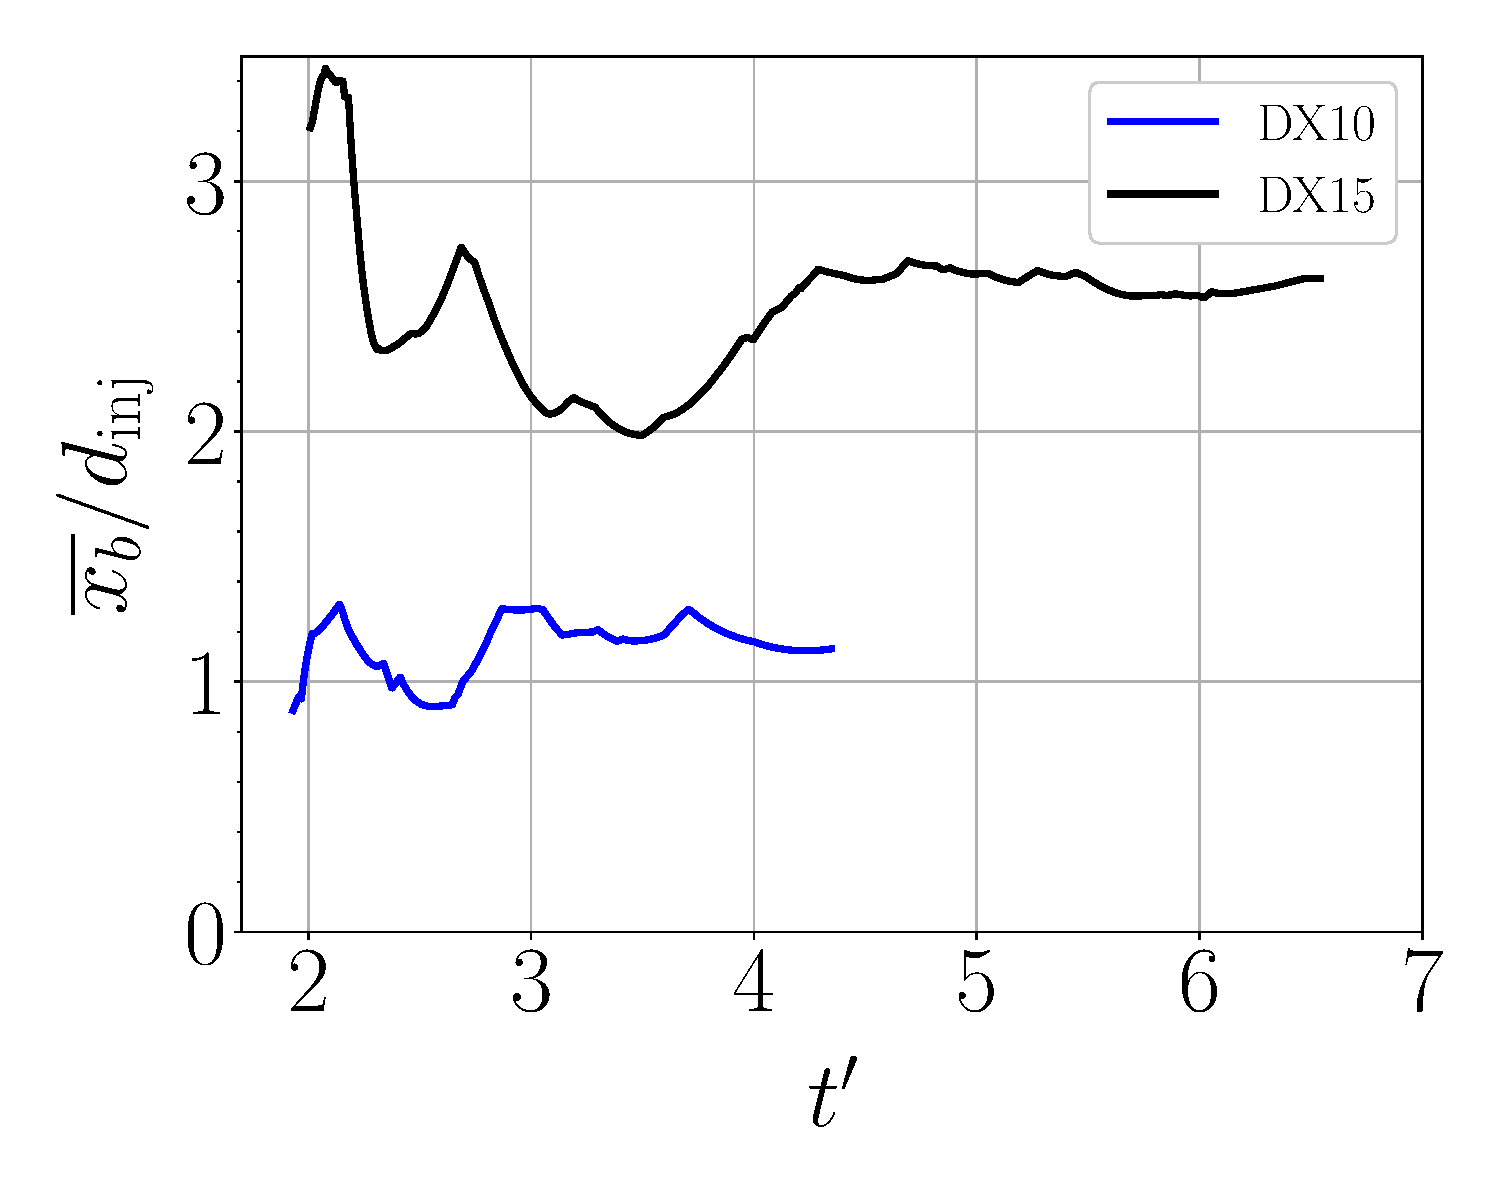
\includegraphics[scale=0.225]{./part3_applications/figures_ch8_resolved/results_dense_core_modeling/convergence_mean_xb}
\end{subfigure}
\hfill
\begin{subfigure}[b]{0.3\textwidth}
	\flushleft
   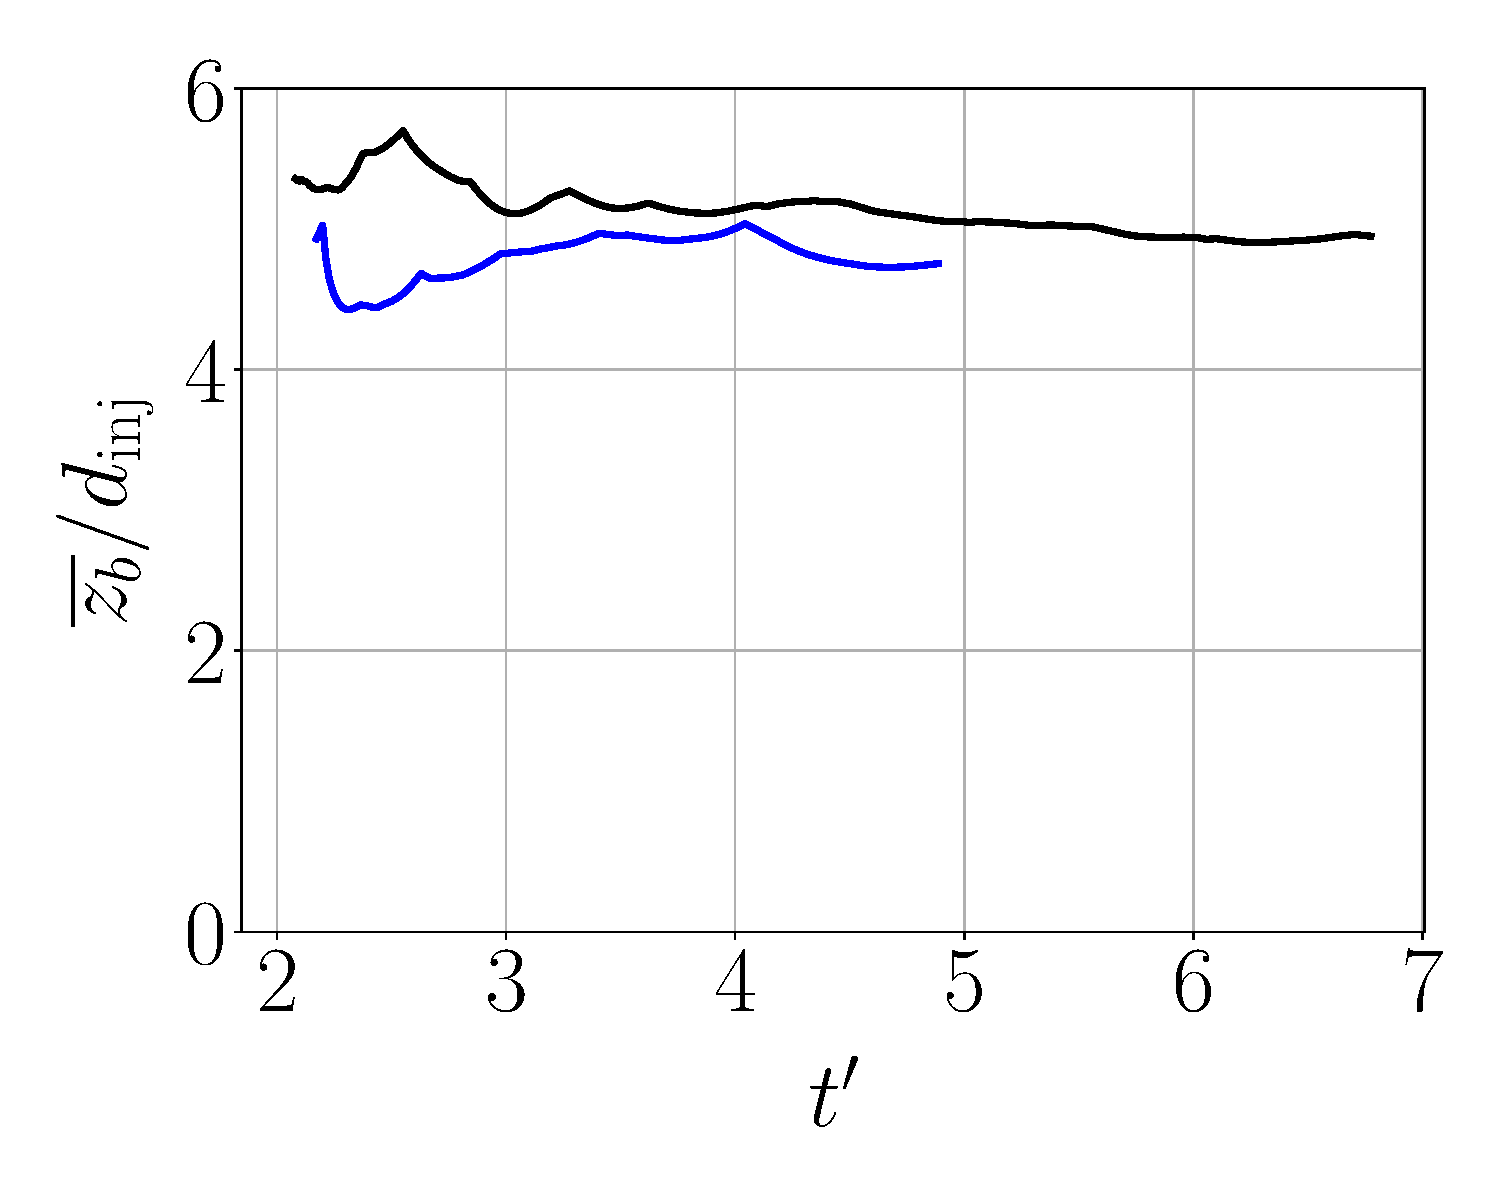
\includegraphics[scale=0.225]{./part3_applications/figures_ch8_resolved/results_dense_core_modeling/convergence_mean_zb}
\end{subfigure}
\hfill
\begin{subfigure}[b]{0.3\textwidth}
	\flushleft
   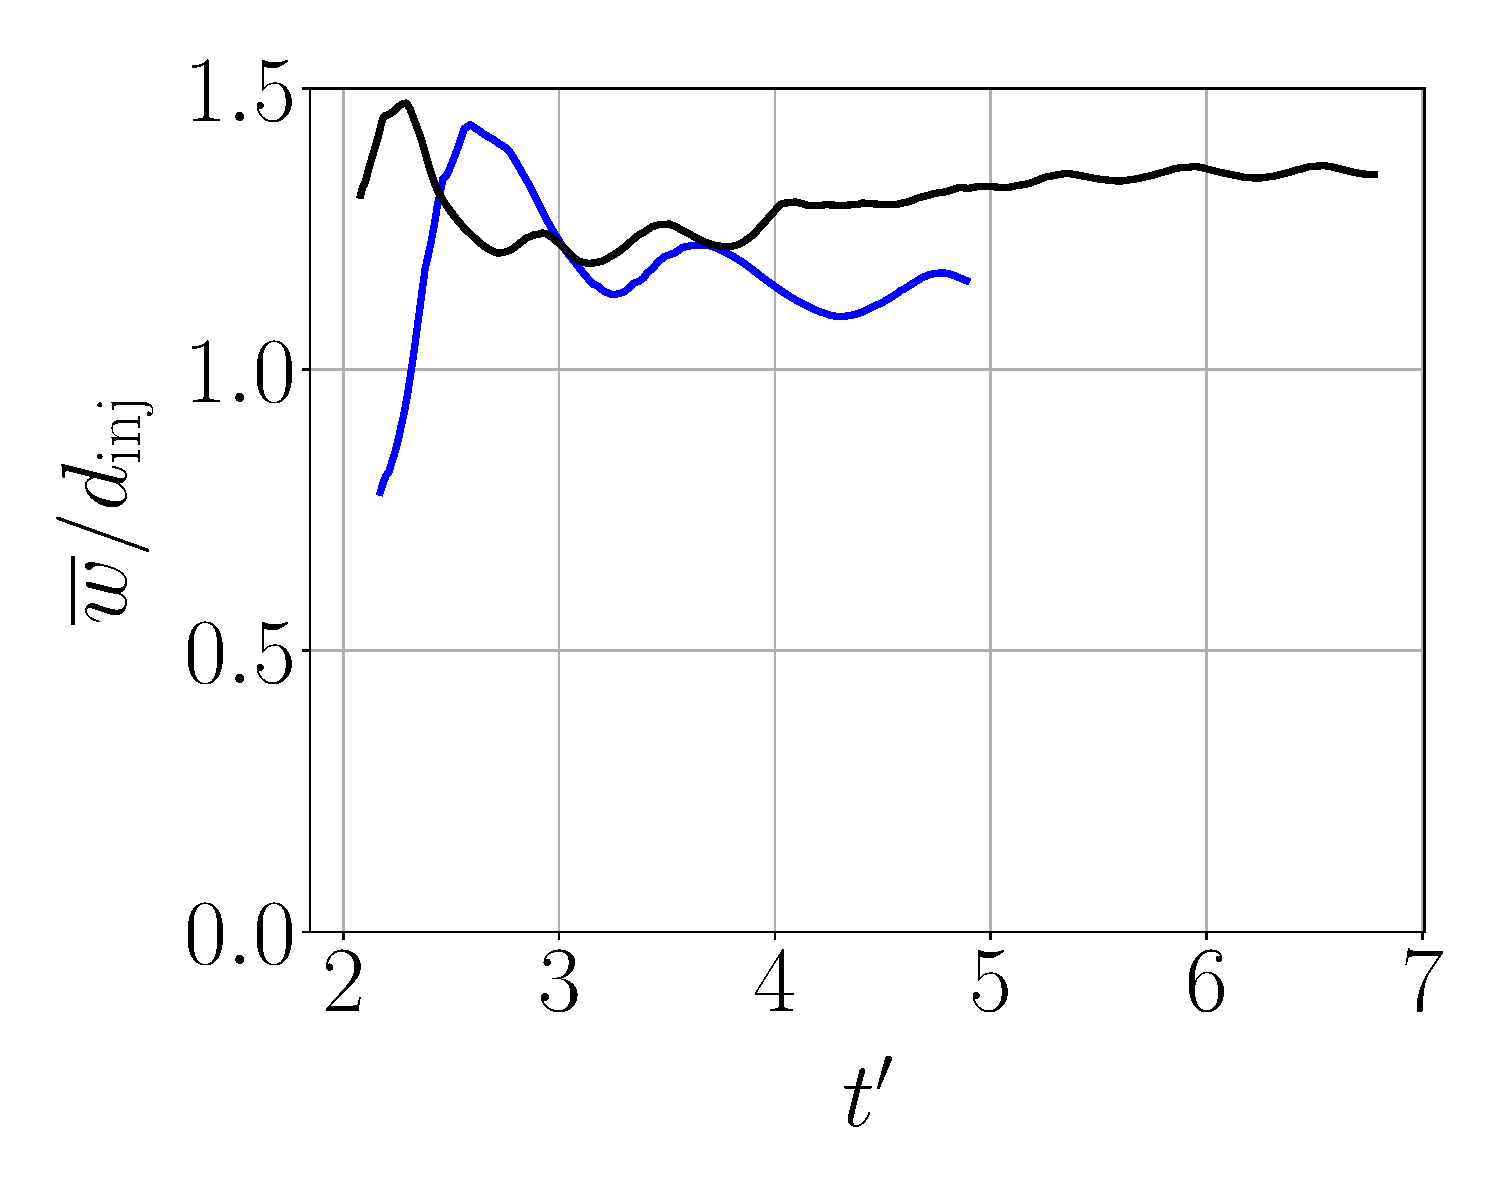
\includegraphics[scale=0.225]{./part3_applications/figures_ch8_resolved/results_dense_core_modeling/convergence_mean_width}
\end{subfigure}
   \caption{Evolution of mean geometric parameters of BIMER dense core}
\label{fig:BIMER_DC_mean_parameters_convergence}
\end{figure}

\begin{figure}[ht]
\flushleft
\begin{subfigure}[b]{0.45\textwidth}
	\centering
   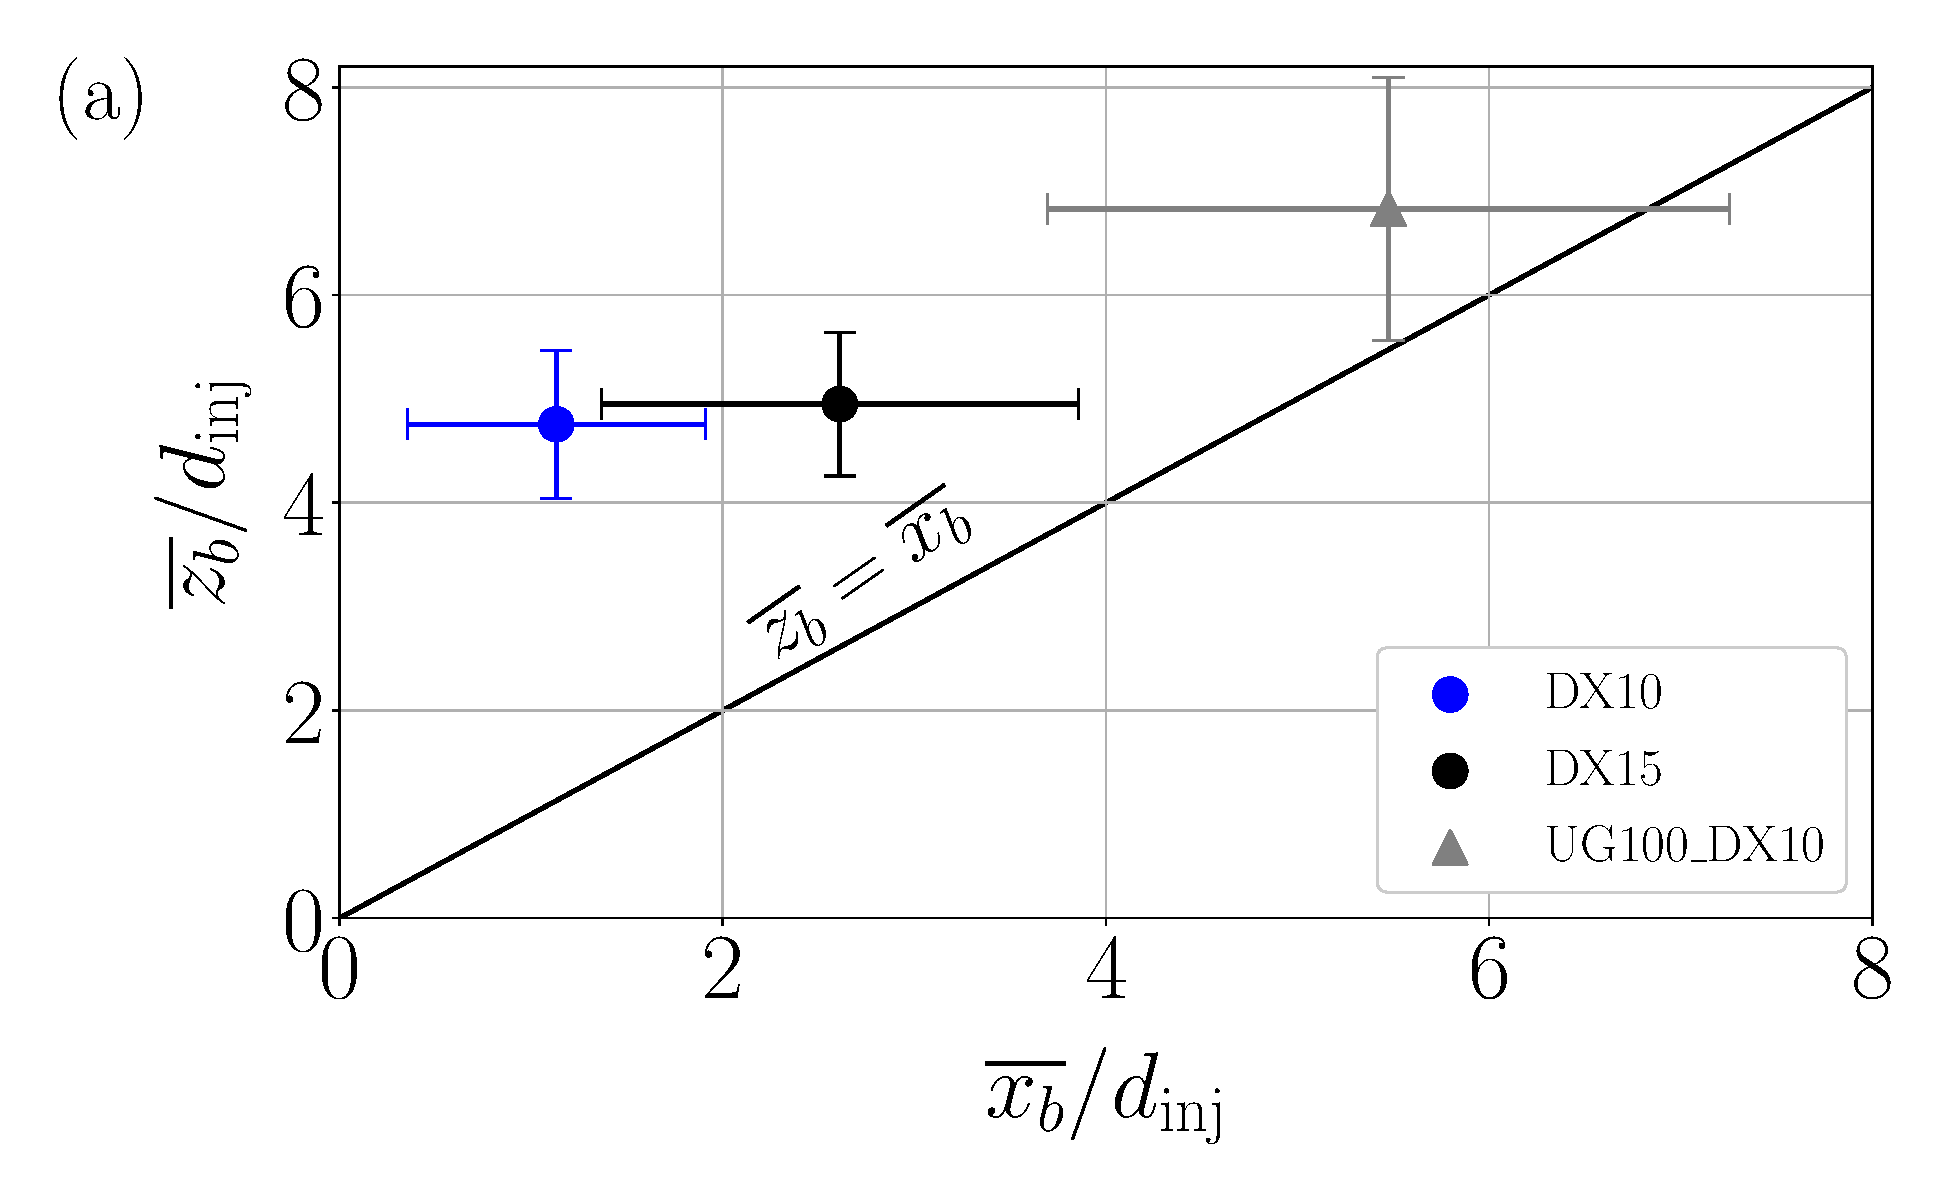
\includegraphics[scale=0.25]{./part3_applications/figures_ch8_resolved/results_dense_core_modeling/map_xb_zb}
   \label{fig:BIMER_dense_core_mean_parameters_scatterplots_zb_xb}
\end{subfigure}
%\hfill
\hspace{0.25in}
\begin{subfigure}[b]{0.45\textwidth}
	\centering
   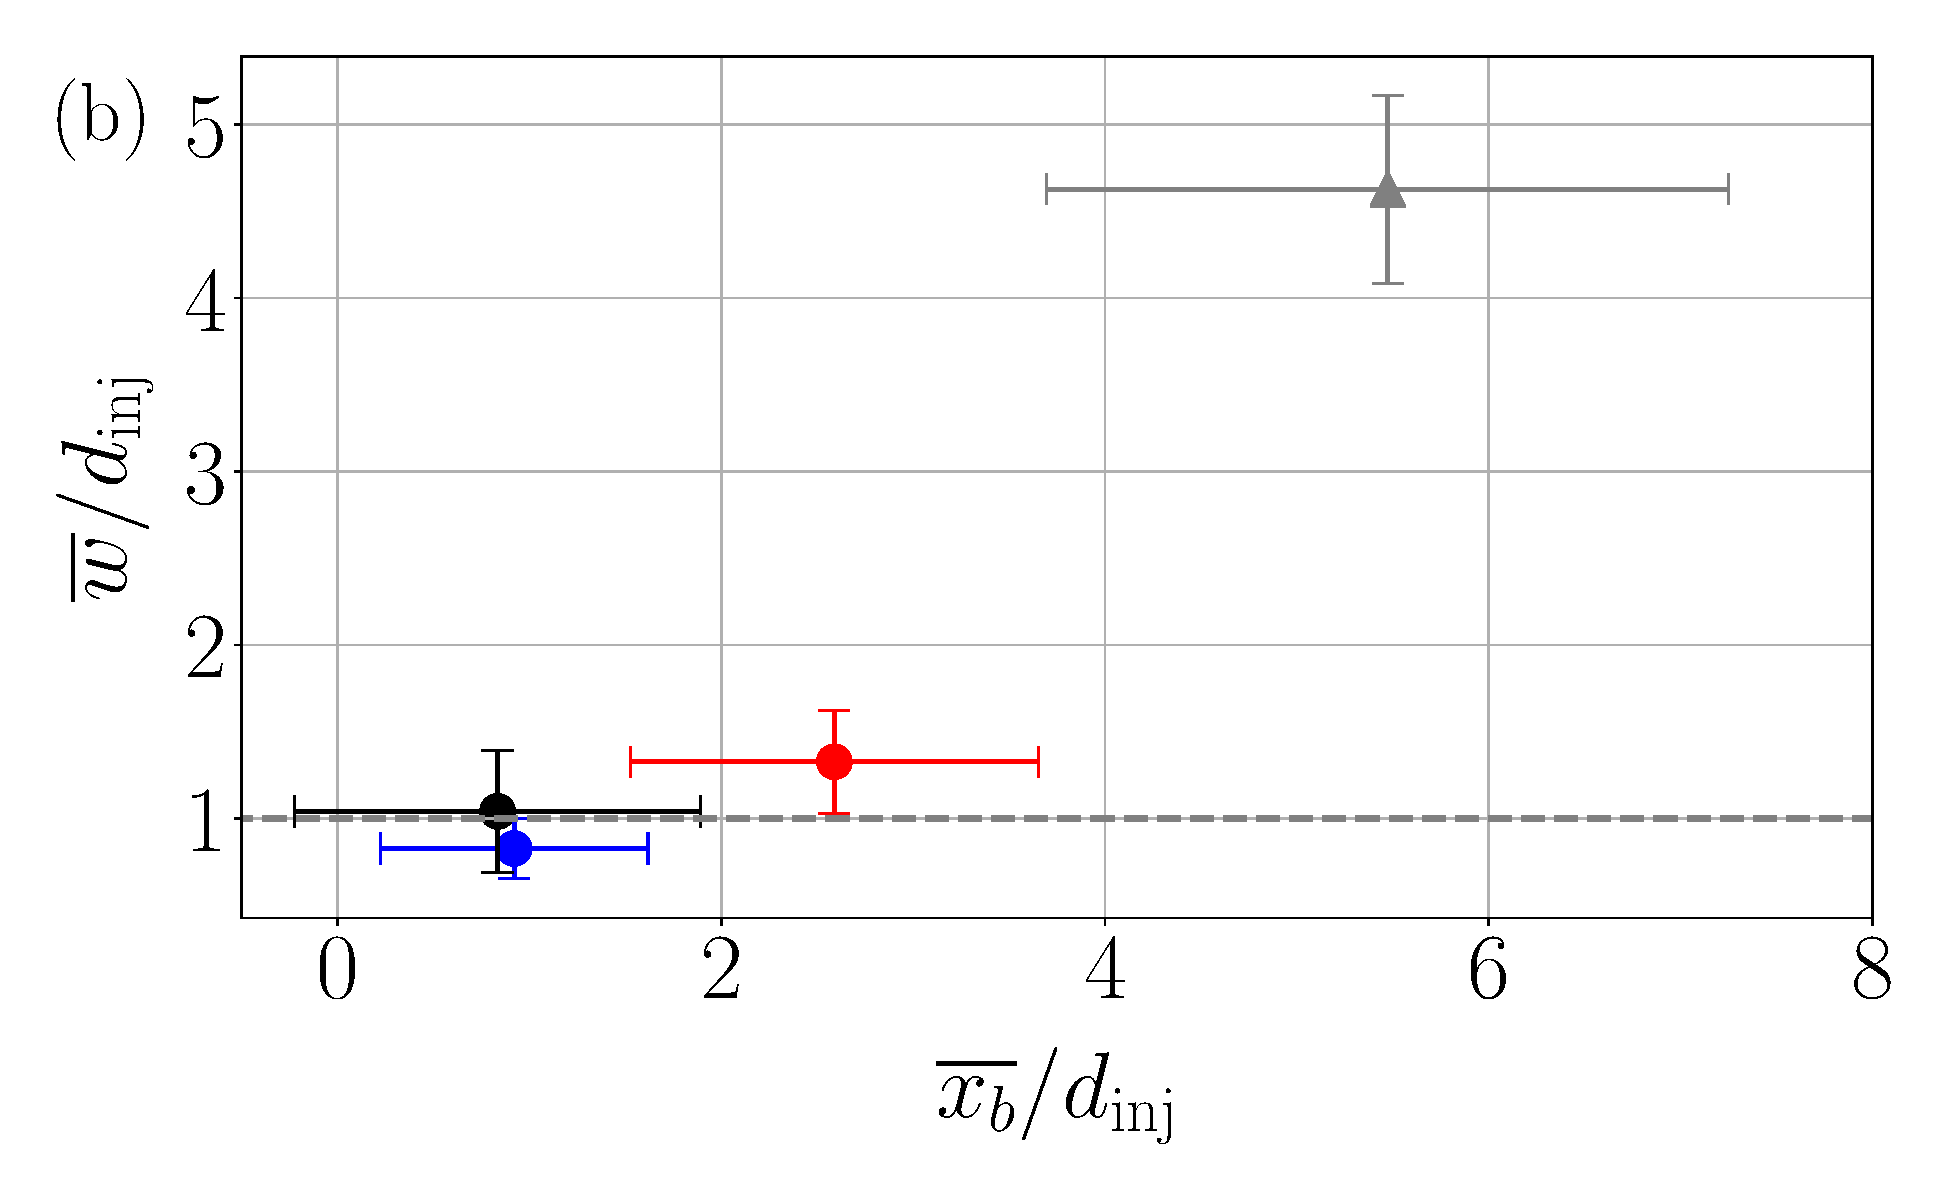
\includegraphics[scale=0.25]{./part3_applications/figures_ch8_resolved/results_dense_core_modeling/map_xb_width}
   \label{fig:BIMER_dense_core_mean_parameters_scatterplots_w_xb}
\end{subfigure}
   \vspace*{-0.30in}
\caption{Mean values for the BIMER dense core geometric parameters}
\label{fig:BIMER_DC_mean_parameters_scatterplots}
\end{figure}

%\begin{table}[!h]
%\centering
%\caption{BIMER dense core mean lengths $L_\mathrm{DC}$ and widths $w$ from JICF simulations performed}
%\begin{tabular}{cccc}
%\thickhline
%\textbf{Case} &  DX07 & DX10 & DX15  \\
%\hline
%$L_\mathrm{DC}/d_\mathrm{inj}$ & 4.66 & 4.83 & 5.44  \\
%$w/d_\mathrm{inj}$ & 0.83 & 1.04 & 1.33  \\
%\thickhline
%\end{tabular}
%\label{tab:BIMER_L_DC_values}
%\end{table}

\begin{table}[!h]
\centering
\caption{BIMER dense core mean lengths $L_\mathrm{DC}$ and widths $w$ from JICF simulations performed}
\begin{tabular}{cccc}
\thickhline
\textbf{Case} &   DX10 & DX15  \\
\hline
$L_\mathrm{DC}/d_\mathrm{inj}$ & 4.83 & 5.44  \\
$w/d_\mathrm{inj}$ & 1.04 & 1.33  \\
\thickhline
\end{tabular}
\label{tab:BIMER_L_DC_values}
\end{table}


\subsection{Force determination in BIMER dense core}

In order to estimate the net force exerted to the dense core to be imposed as initial input parameter to the ALM in dispersed phase simulations, the same procedure as detailed in $\S$\ref{eq:ch5_subsec_force_determination_JICF} is applied to BIMER. Results obtained for both simulations performed are summarized in Table \ref{tab:BIMER_dense_core_pressures_and_force_parameters}. The dense core surfaces obtained by applying Eq. (\ref{fig:extraction_methodology_mean_DC}) with the values from Table \ref{tab:BIMER_L_DC_values}, and the dense core net force obtained with Eq. (\ref{eq:ALM_Fp_calculation_simplified}), are also summarized.


\begin{table}[!h]
\centering
\caption{Pressures and net dense core surfaces in BIMER simulations}
\begin{tabular}{ccccc}
\thickhline
\textbf{Case} & $p_\mathrm{windward}$ [Pa] & $p_\mathrm{leeward}$ [Pa] & $S_\mathrm{DC}$ [mm$^2$]& $|\boldsymbol{F}_\mathrm{DC}|$ [mN] \\
\thickhline 
%DX07  & 2340 & 1550 & 0.38 & 0.1 \\
DX10 & 2020 & 1475 & 0.47 & 0.25 \\
DX15 & 2340 & 1550 & 0.59 & 0.45 \\
\thickhline
\end{tabular}
\label{tab:BIMER_dense_core_pressures_and_force_parameters}
\end{table}

\subsection{Turbulent structures in the gaseous field}
\label{subsec:ch8_turbulent_structures_BIMER}

The disturbance effect of the BIMER dense core towards the gaseous phase is analyzed in this section. Figure \ref{fig:streamlines_BIMER_from_dump} illustrates this perturbation phenomenon through the mean 3D streamlines around the jet, which shows that characteristical turbulent structures  observed in liquid JICFs, such as horseshoe vortices and recirculation zone behind the liquid column, are found. Both of these features were observed both experimentally and in the JICF simulations of Chapter \ref{ch5:jicf_resolved_simulations}. When compared to those, the recirculation zone in BIMER is be located closer to the wall and with a smaller extension. The perturbation effect on the gaseous phase is further analyzed by looking at the planes shown in Figure \ref{fig:BIMER_sps_with_gaseous_planes}. 

\begin{figure}[h!]
	\centering	\includeinkscape[inkscapelatex=false,scale=0.5]{./part3_applications/figures_ch8_resolved/turbulent_structures/streamlines_BIMER}
	\vspace*{-0.5in}
	\caption{Streamlines in BIMER, case DX10}
	% NOTA: figura de pilotage 2021_02_04
		\label{fig:streamlines_BIMER_from_dump}
\end{figure}


\begin{figure}[h!]
	\centering	\includeinkscape[inkscapelatex=false,scale=0.8]{./part3_applications/figures_ch8_resolved/turbulent_structures/BIMER_sps_with_gaseous_planes}
	\caption{Jet from BIMER case DX10 showing planes to study the gaseous phase}
	\label{fig:BIMER_sps_with_gaseous_planes}
\end{figure}

The mean axial velocity fields at plane $y_c = 0$ are shown in Figure \ref{fig:BIMER_turbulent_structures_plane_y0}. The mean liquid region is denoted by the grey area: this region deviates in the fine case to a lower extent than in the coarse one, as also observed in the instantaneous snapshots of Figure \ref{fig:BIMER_jet_establishment}, which leads then to an earlier breakup point as demonstrated by the shorter dense core lengths from Table \ref{tab:BIMER_L_DC_values}. Regarding the gaseous field, the perturbation effect of the dense core is clearly noticed by the decelerations created by the crossflow. A region with negative velocity is found attached to the wall right upstream the dense core for both resolutions, corresponding to the horseshoe vortex as also visualized in Figure \ref{fig:streamlines_BIMER_from_dump}. Recirculation regions are also observed in the leeward side, being however different in each case: DX10 displays a small vertical region with small thickness in the axial direction, probably not converged with the physical time simulated, while DX15 displays a larger recirculation bubble more inclined along the liquid column due to the jet's deviation  and with larger width than the first case. In both cases, however, the recirculation bubbles present small thicknesses in relation to the injection diameter with respect to the recirculation bubbles obtained  for the non-swirled in Figure \ref{fig:JICF_sps_lines_y0_along_x_ux_mean}. This might be attributed to a lower momentum flux ratio in the BIMER case with respect to the previous JICF: $q = 2$ for the former with respect to $q = 6$ for the latter. A lower $q$ supposses a lower penetration, with might lower down the location of the recirculation region and reduce its strength similar to the flow behind bluff bodies \citepColor[asami_improvement_2021]. The recirculation zone is also affected by the geometry of the body, which in the case of liquid jets in crossflow is complex, unsteady and differs among both jets simulated (see the instantaneous topologies in Figure \ref{fig:jet_air_interaction_up_and_skeleton} right and \ref{fig:BIMER_jet_air_interaction_up_and_skeleton} right). Previous studies about such parametrical influences on JICF recirculation zones have not been performed to the knowledge of the author, and are not ellucidated in this thesis. 

 %The the recirculation region is also affected by the gas Reynolds number $Re_g$, which for the case of BIMER, $Re_g \sim \mathcal{O} \left( 10^4 \right)$, is lower than for the case of the JICF from Chapter \ref{ch5:jicf_resolved_simulations}, where $Re_g \sim \mathcal{O} \left( 10^6 \right)$: lower $Re_g$ reduces the length and strengh of recirculation zones behind obstacles ()

\vspace*{-0.5in}


\begin{figure}[ht]
\centering
   \includeinkscape[inkscapelatex=false,scale=0.25]{./part3_applications/figures_ch8_resolved/turbulent_structures/planes_y_ux_mean}
%\vspace{-0.5in}
\caption[Mean axial velocity at plane $y = 0$ mm]{Mean axial velocity at plane $y = 0$ mm. Black lines with arrows are in-plane mean streamlines; the white solid line indicates the contour $\overline{u} = 0$ which delimites the recirculation bubble. The grey area indicates the mean liquid region, identifed as $\overline{\psi} > 0.5$}
\label{fig:BIMER_turbulent_structures_plane_y0}
\end{figure}


The mean axial velocity profiles along the lines $z_c = 0.3, 1.5$ mm are plotted in Figure \ref{fig:BIMER_sps_lines_y0_along_x_ux_mean}. The dashed black line shows the mean profile for the single-phase simulation without liquid (i.e. undisturbed gaseous phase due to the present of the jet dense core). Near the wall ($z_c = 0.3$ mm), the perturbance effect is strong and the difference with respect to the single-phase case is high. A region with negative axial velocity is observed at the near field region, which corresponds to the recirculation bubble seen in Figure \ref{fig:BIMER_turbulent_structures_plane_y0}. The difference with respect to the single-phase decreases further downstream but the gaseous field of the two-phase simulations does not reach the same tendency again, showing low-velocity oscillations with $x_c$ that are maintained further downstream. Further from the wall ($z_c = 1.5$ mm), the disturbance is also close to the jet but the velocity field relaxes quickly and reaches the same tendency of the single-phase simulation further downstream, at $x_c \sim 11$ mm. For all cases, both resolved atomization simulations recover the same trends in the perturbed fields with quantitative differences observed due to the different jets resolved: the amplitude of the variations with $x_c$ is in general stronger for case DX10. Figure \ref{fig:BIMER_sps_lines_y0_along_z_ux_mean} plots then the velocity fields along the vertical coordinate $z_c$ represented in Figure \ref{fig:BIMER_turbulent_structures_plane_y0}, showing that differences with respect to a pure gaseous simulation are higher in the near-wall region but get closer further upstream, with again differences among resolutions. These differences get lower further dowstream at $x_c = 40$ mm, but still being of the order of $20~\mathrm{m~s}^{-1}$ which could greatly affect affect the secondary atomization of the droplets in the dispersed-phase simulations if the gaseous perturbations is not properly perturbed. It is worth to note that the sampling planes range from $x_c = 1.5$ to $3$ mm (see Figure \ref{fig:BIMER_local_FoR_and_sampling_planes}), therefore droplets sampled are located within this highly perturbed region. Lagrangian particles injected in the dispersed-phase simulations should ideally \textsl{see} a highly perturbed gaseous field right after injection, which is not actually possible since such a complex gaseous field cannot be accurately retrieved with ALM (\hl{see Chapter} \ref{ch9:BIMER_lagrangian}).

\clearpage


\begin{figure}[ht]
\flushleft
\begin{subfigure}[b]{0.45\textwidth}
	\flushleft
   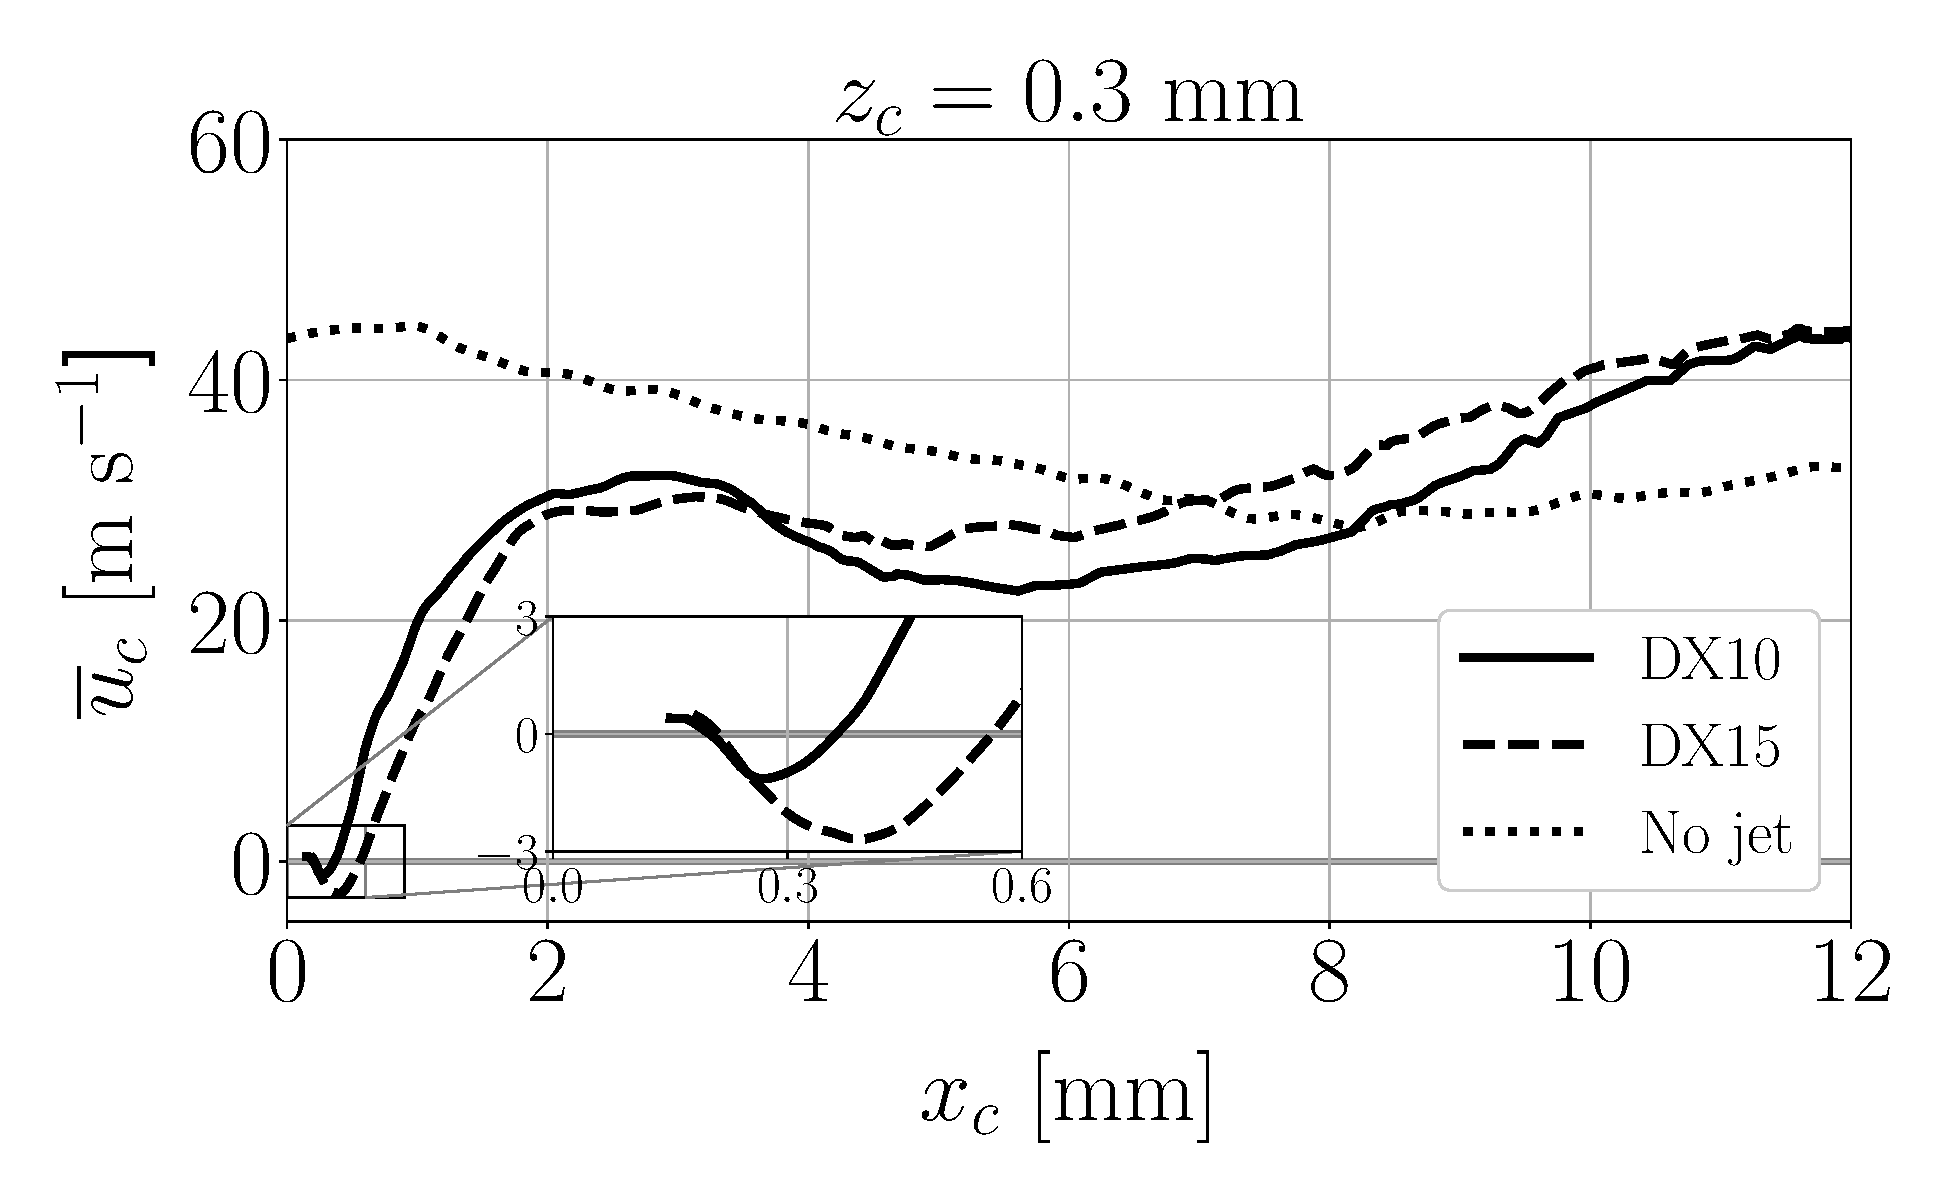
\includegraphics[scale=0.25]{./part3_applications/figures_ch8_resolved/turbulent_structures/line_y0_along_x_zlow}
   %\caption{}
   %\label{} 
\end{subfigure}
\hspace{0.4in}
\begin{subfigure}[b]{0.45\textwidth}
	\flushleft
   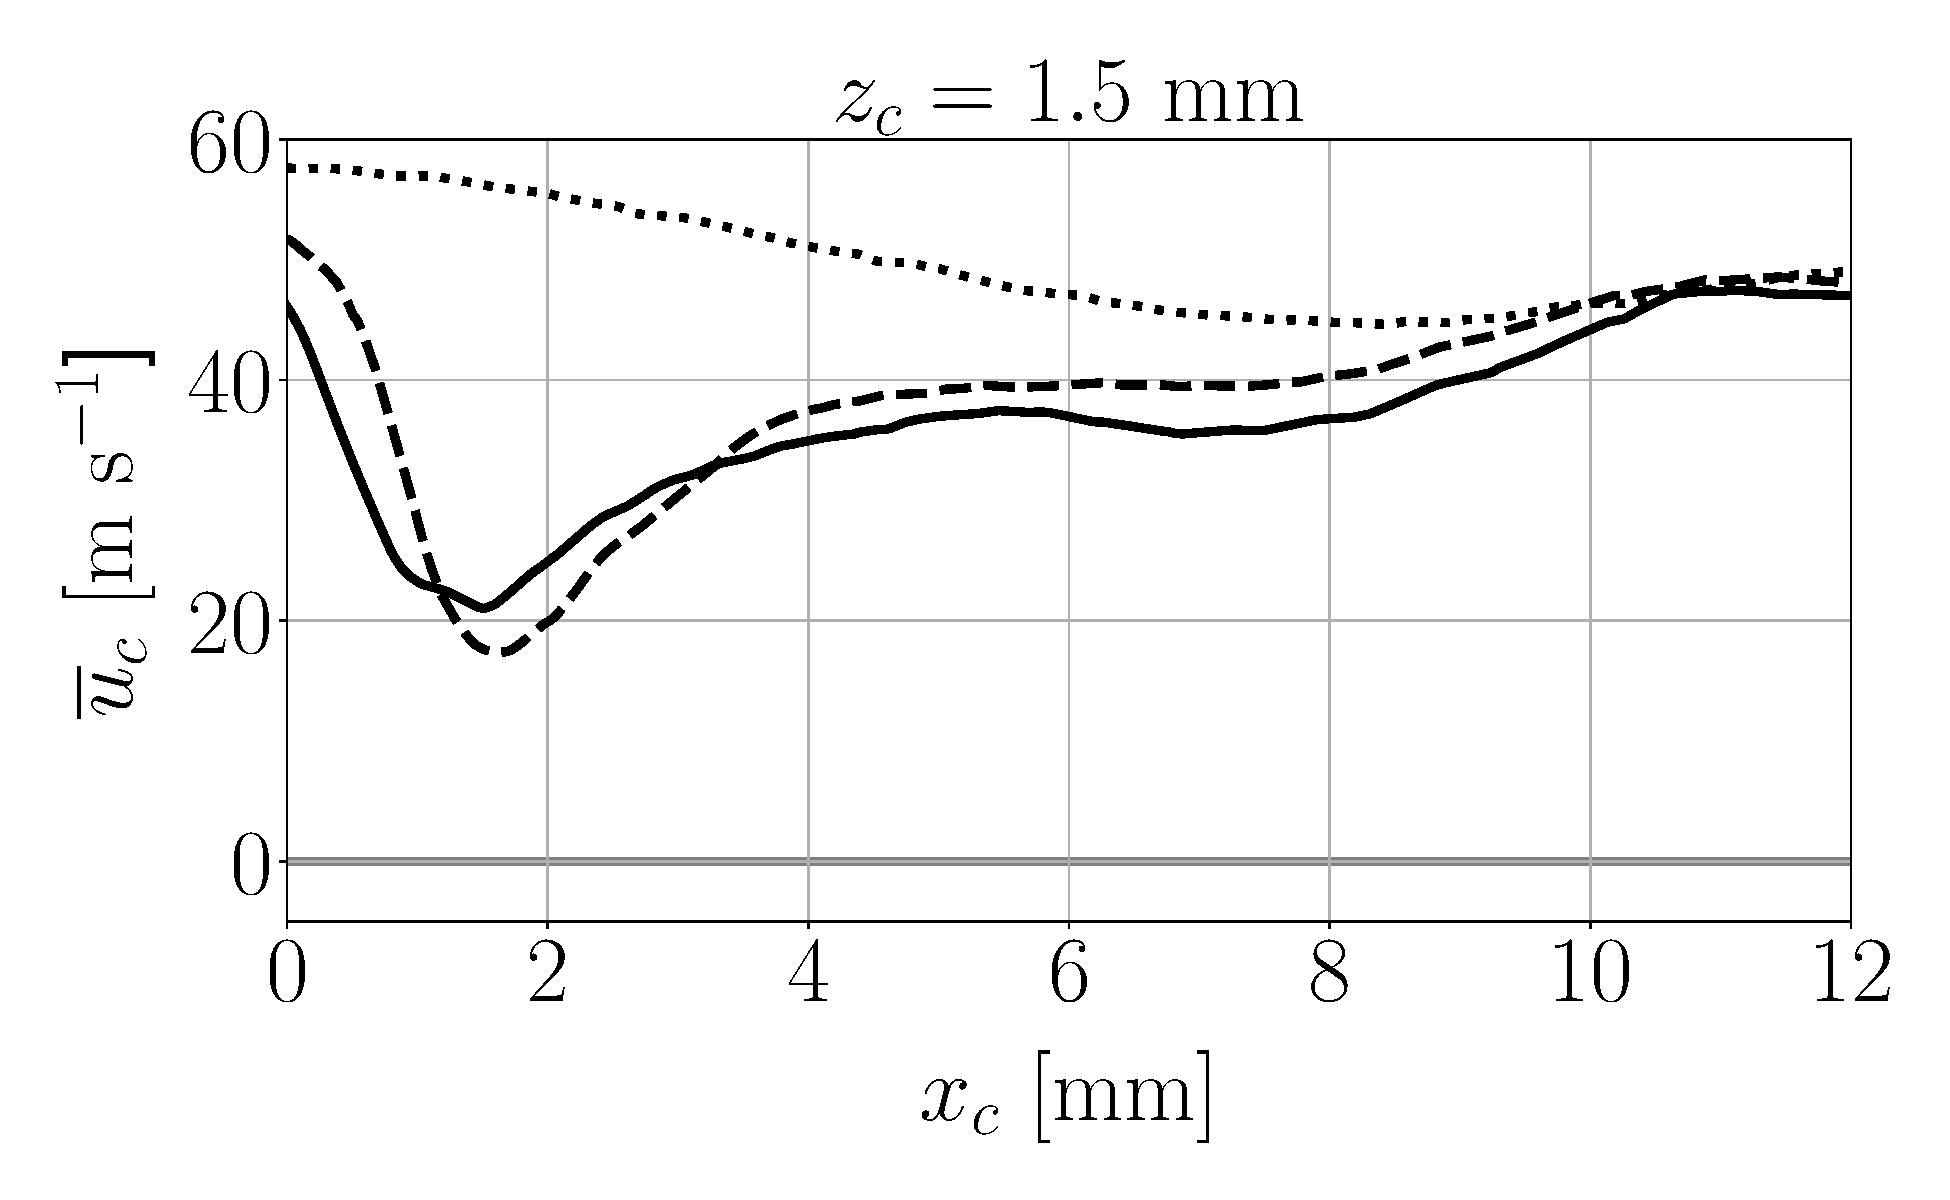
\includegraphics[scale=0.25]{./part3_applications/figures_ch8_resolved/turbulent_structures/line_y0_along_x_zhigh}
   %\caption{}
   %\label{}
\end{subfigure}
\caption{Mean axial velocity evolution along axial coordinate at locations $z_c = 0.3, 1.5$ mm at plane $y_c = 0$ (lines of Figure \ref{fig:BIMER_turbulent_structures_plane_y0})}
\label{fig:BIMER_sps_lines_y0_along_x_ux_mean}
\end{figure}


\begin{figure}[ht]
\centering
   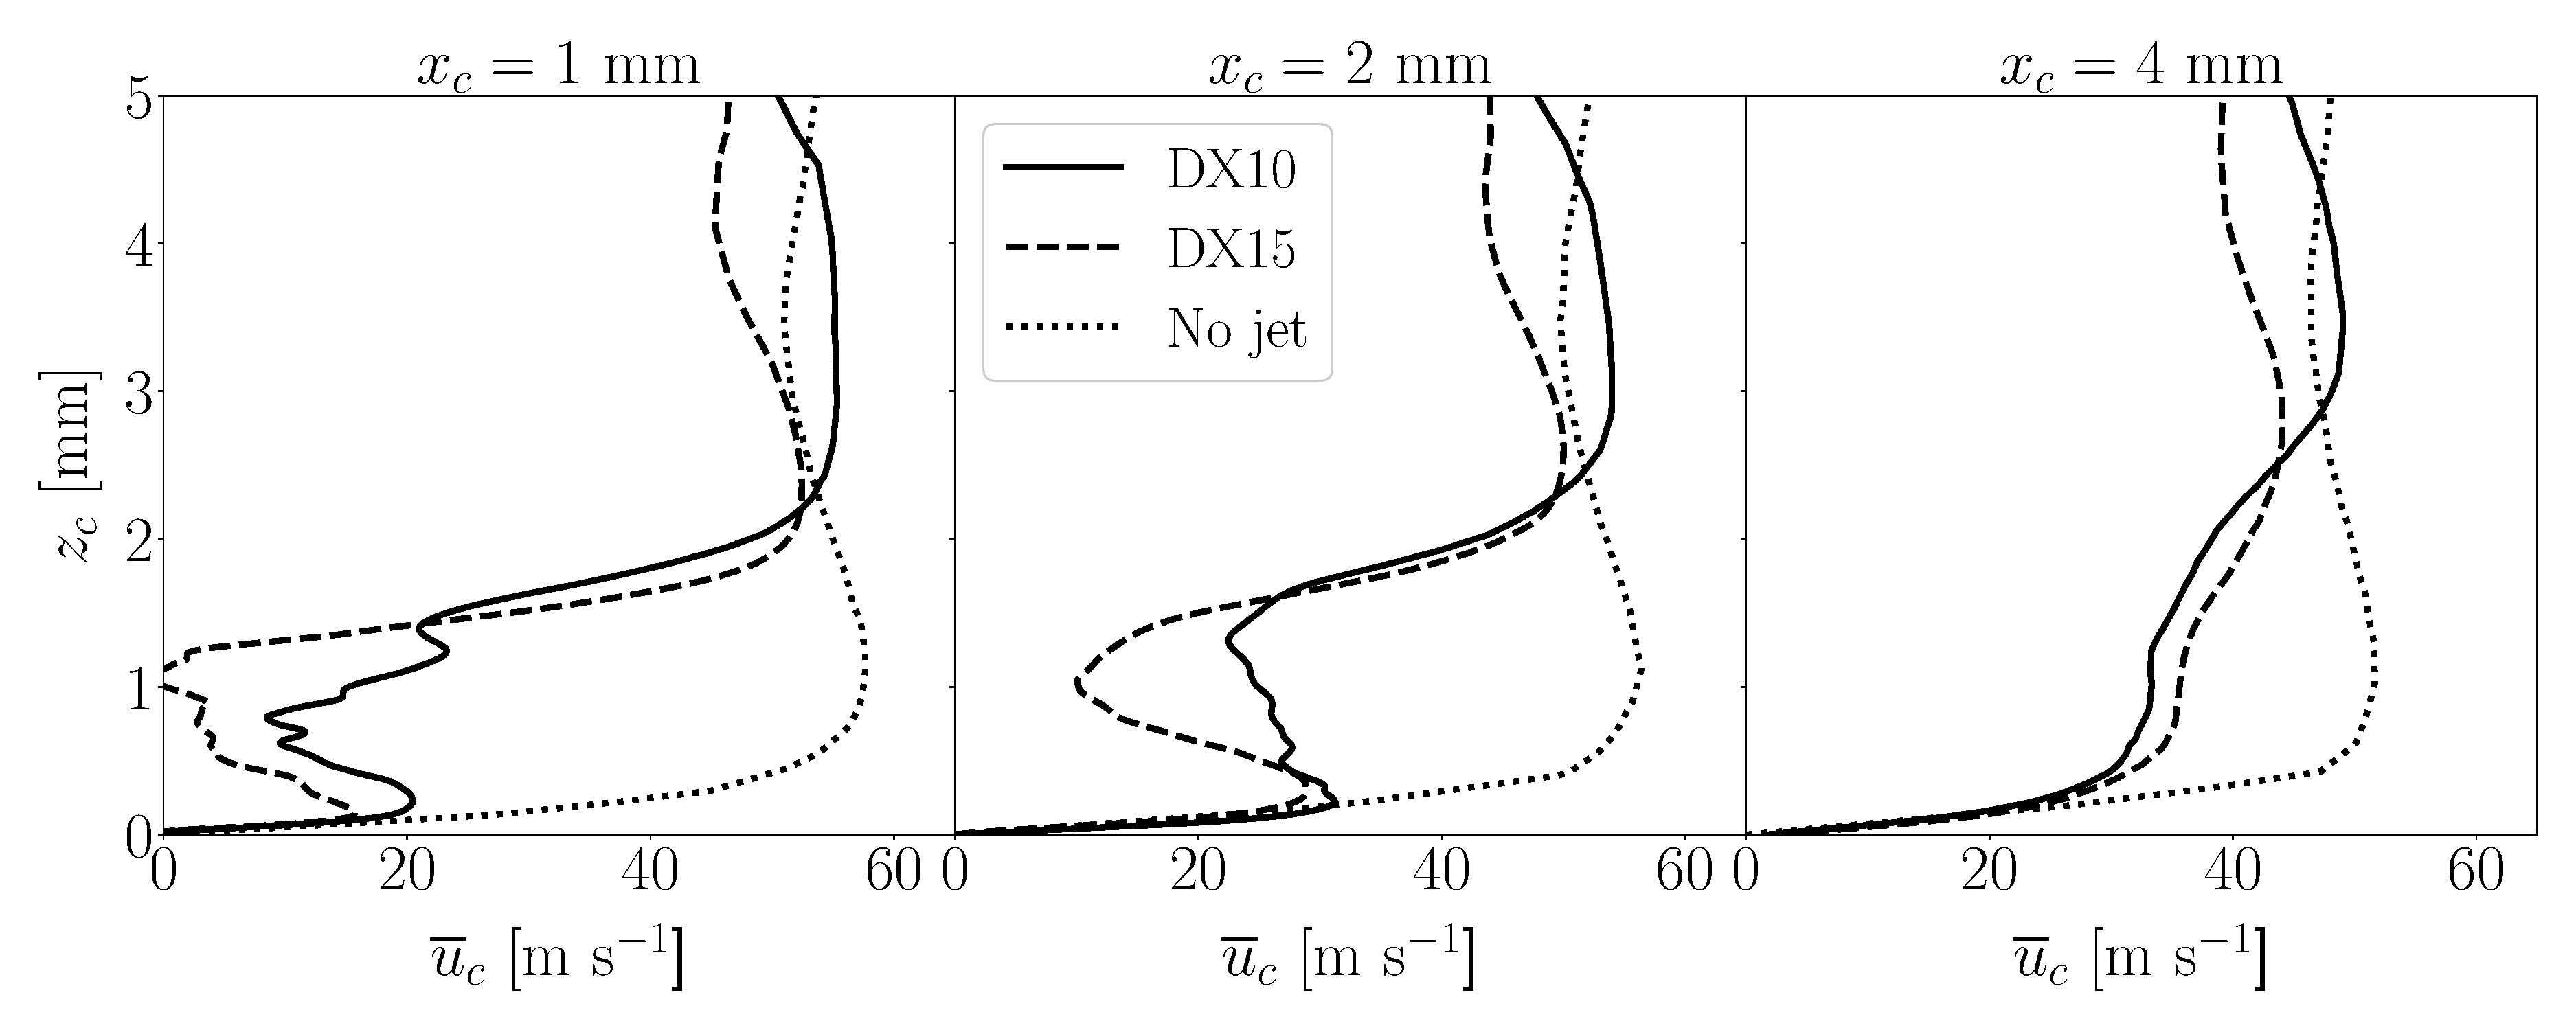
\includegraphics[scale=0.24]{./part3_applications/figures_ch8_resolved/turbulent_structures/lines_y0_along_z_ux_mean}
\caption{Mean axial velocity evolution along vertical coordinate at $x_c = 1, 2, 4$ mm locations of plane $y = 0$ (lines of Figure \ref{fig:BIMER_turbulent_structures_plane_y0})}
\label{fig:BIMER_sps_lines_y0_along_z_ux_mean}
\end{figure}


Planes perpendicular to crossflow $x_c = 1.5, 3$ mm are shown in Figure \ref{fig:BIMER_turbulent_structures_planes_x}. The disturbance effect is clearly seen by the low velocity region at both sides of plane $y_c = 0$. This region is symmetric at plane $x_c = 1.5$ mm for case DX15 but not for the other figures depicted, which show an inclination of the deceleration region towards direction $y_c < 0$. Asymmetry is attributed to the swirl of the jet, which does not create a symmetric velocity field with respect to plane $y_c = 0$.  This behaviour has been observed in other swirled JICF \citemColor[denev_large_2009,terzis_swirl_2011], while tradicitional configurations without swirl always present symmetric gaseous structures (see for instance Figure \ref{fig:JICF_turbulent_structures_planes_x}). Another particular in this configuration is related to the vortical structures, which are not captured in all cases and, when present, are asymmetric with respect to plane $y_c = 0$. Case DX10 at $x_c = 1.5$ mm shows two different vortices that constitute the counter-rotating vortex pair (CVP) as also observed in Figure \ref{fig:JICF_turbulent_structures_planes_x}. Further downstream at $x_c = 3$ mm the vortex located at $y_c > 0$ has reached the wall and dissipated, while the one at $y_c < 0$ has moved further away from the centerline, resulting in just one vortex. For case DX15, at $z_c = 1.5$ mm only one vertex at $y_c < 0$ is captured while further downstream no vortices are observed. Similar asymmetric vortical structures and their evolution over the axial coordinate $x_c$ have been observed in previous studies of liquids jet in crossflow where swirl is imposed in the liquid nozzle \citemColor[denev_large_2009,terzis_swirl_2011], which have shown larger asymmetries when the swirl number is increased at low values below 1 (the swirl number in the BIMER configuration is $S_w \sim 1$). Unfortunately, vortical structures in such planes on highly-swirled JICF or configurations where swirl is imposed to the gaseous phase are not available to the knowledge of the author, so a comparison in similar comparisons cannot be performed.

\clearpage 

% Looking at the streamlines, one of the first observations is that the classical CVP pairs typically observed in JICF configurations, visualized in the JICF configuration of DLR in Figure \ref{fig:JICF_turbulent_structures_planes_x}, are not present in BIMER. A possible explanation of missing CVPs in due to the lack of jet deflection towards the axial direction, which was notorious in the classical JICF (see for instance Figure \ref{fig:JICF_establishment_UG100_lateral}) but which is not very pronounced in BIMER, as shown in Figure \ref{fig:BIMER_jet_establishment}. \citeColor[broadwell_structure_1984] argued that the strength of the CVPs is dependent on the momentum transferred to the crossflow by the jet; later, \citeColor[karagozian_analytical_1986] confirmed this statement while also showing that this momentum transfer is not relevant until the jet has been deflected by the crossflow. Since in the present results the BIMER liquid jet does not deflect to a large excent towards the crossflow direction, this hypothesis might explain the absence of CVPs found in the simulations.


%\vspace*{1in}

\begin{figure}[ht]
\centering
   \includeinkscape[inkscapelatex=false,scale=0.30]{./part3_applications/figures_ch8_resolved/turbulent_structures/planes_x_ux_mean}
\caption[Mean axial velocity at planes $x_c/d_\mathrm{inj} = 5, 10$]{Mean axial velocity at planes $x_c/d_\mathrm{inj} = 5, 10$, showing in-plane mean streamlines. The vertical, white line corresponds to plane $y_c = 0$}
%{Mean axial velocity at planes $x = 5, 10$ mm. Black lines with arrows are in-plane mean streamlines. Instantaneous jets for each case are shown in transparent blue.}
\label{fig:BIMER_turbulent_structures_planes_x}
\end{figure}

Figure \ref{fig:BIMER_sps_lines_iso-x_along_y_ux_mean} shows the quantitative evolution of mean axial velocity along the lines plotted in Figure \ref{fig:BIMER_turbulent_structures_planes_x}. The presence of the liquid jet creates a deceleration region in the gaseous phase at the central region and acceleration of the gas further away. The disturbance is stronger closer to the jet nozzle ($x_c = 1.5$ mm) and weaker further away ($x_c = 3$ mm), where the lines with and without liquid get closer. Asymmetry is also observed as the lowest velocities: while in a traditional jet the largest deceleration is located at the centerline (see for instance Figure \ref{fig:JICF_sps_lines_iso-x_along_y_ux_mean}), in BIMER this peak is observed close to it but shifted to the region $y_c < 0$, and moves further away when the axial distance increases, similarly to cases studied in swirled liquids JICF \citepColor[denev_large_2009]. Furthermore, as $y_c$ decreases below $0$ it is seen that the velocities seem to reach a stable velocity which is closer to the single-phase simulation for case DX10, while for $y_c > 0$ the gaseous velocities continue decreasing as $y_c$ increases. This is due to the location of the injection point within the multi-staged, the gaseous flow velocity decreases with axial direction due to the presence of the channels walls (Figure \ref{fig:BIMER_Umean_profile_with_jet} left).


%It could be thought that the location of the crossflow local coordinate system $\left( x_c, y_c, z_c \right)^T$ depicted in Figure \ref{fig:BIMER_local_FoR_and_sampling_planes} has been wrongly chosen, so that another reference frame would place the deceleration peaks at $y_c = 0$. Effectively, 

.



\begin{figure}[ht]
\centering
\begin{subfigure}[b]{1.0\textwidth}
	\centering
   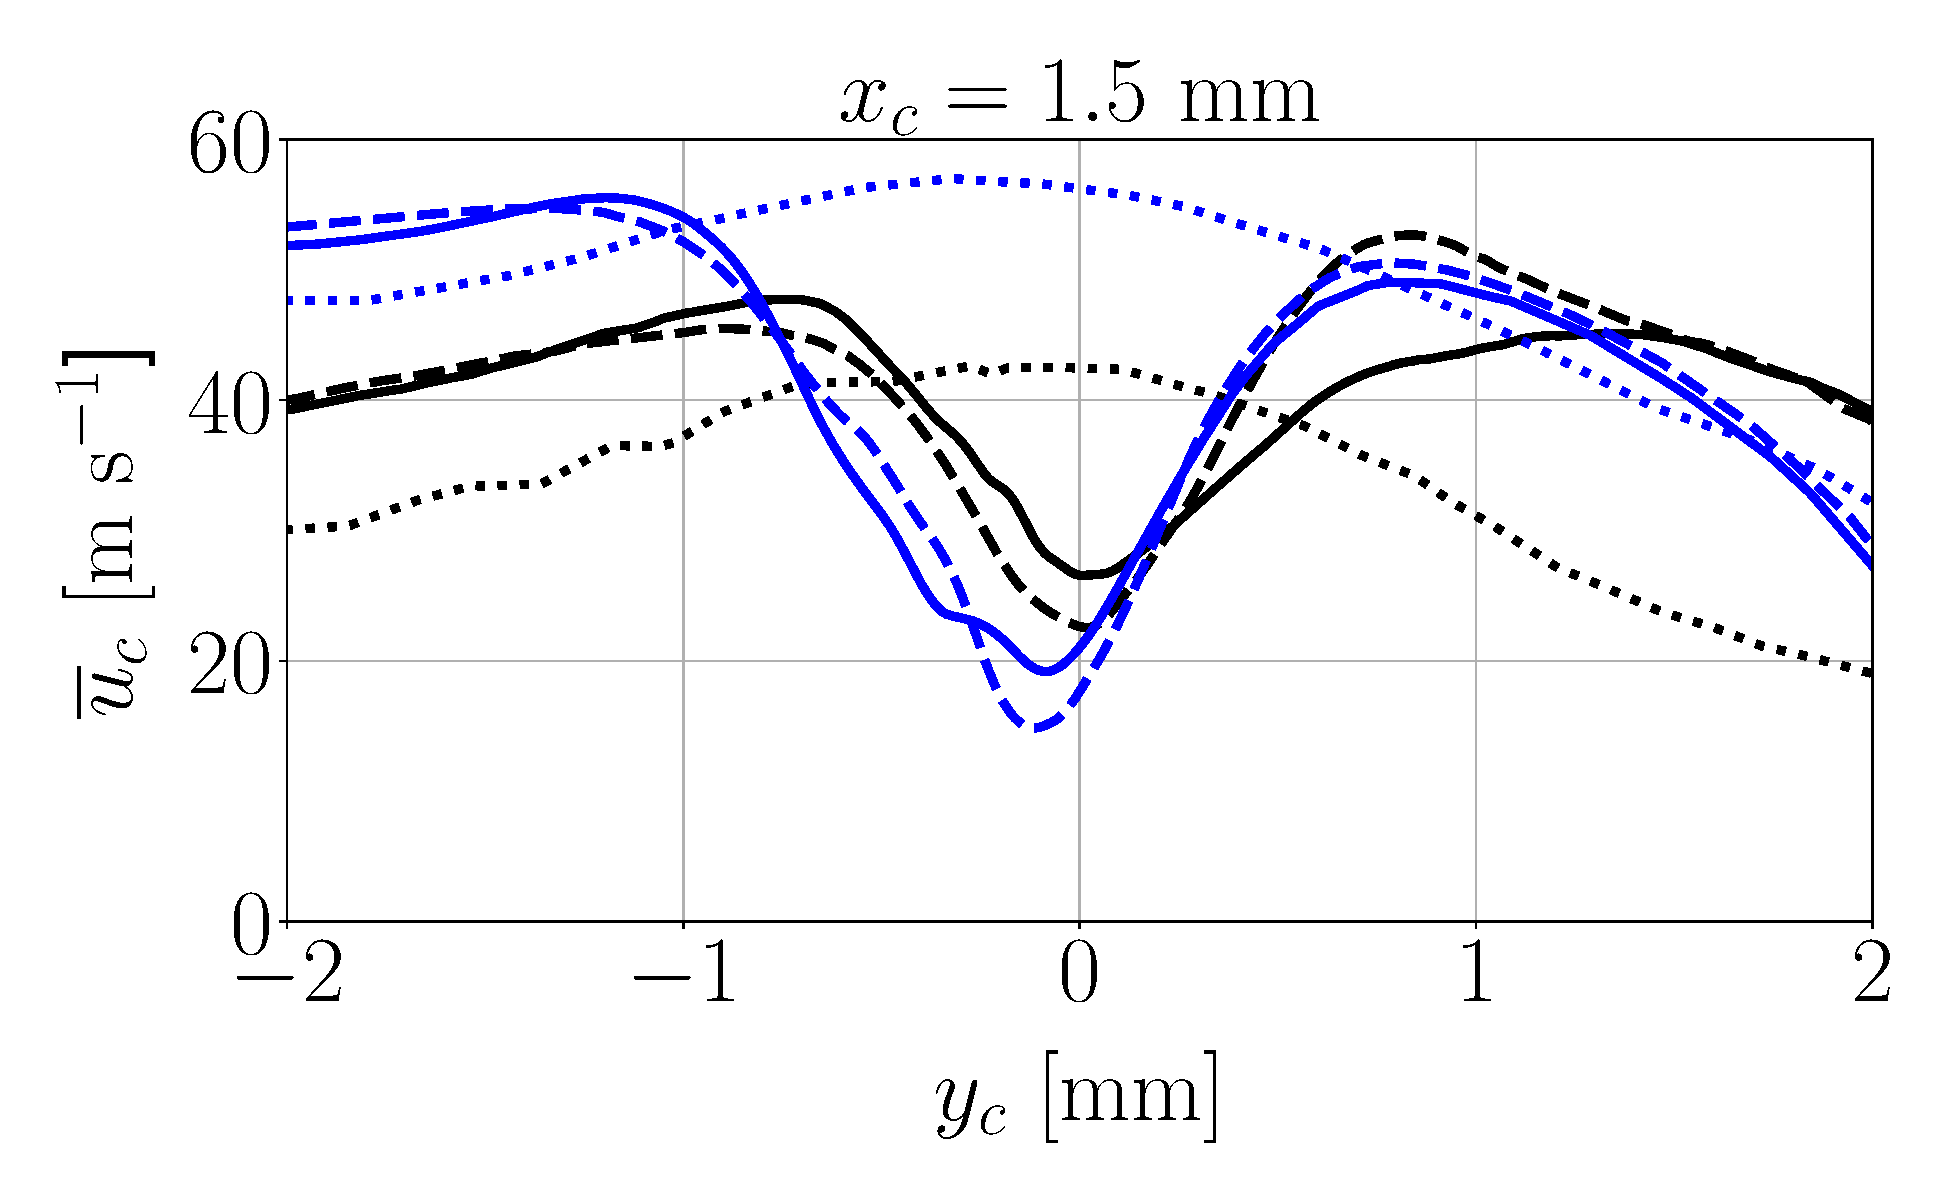
\includegraphics[scale=0.24]{./part3_applications/figures_ch8_resolved/turbulent_structures/lines_iso_x_along_y_plane_x01p5mm}
   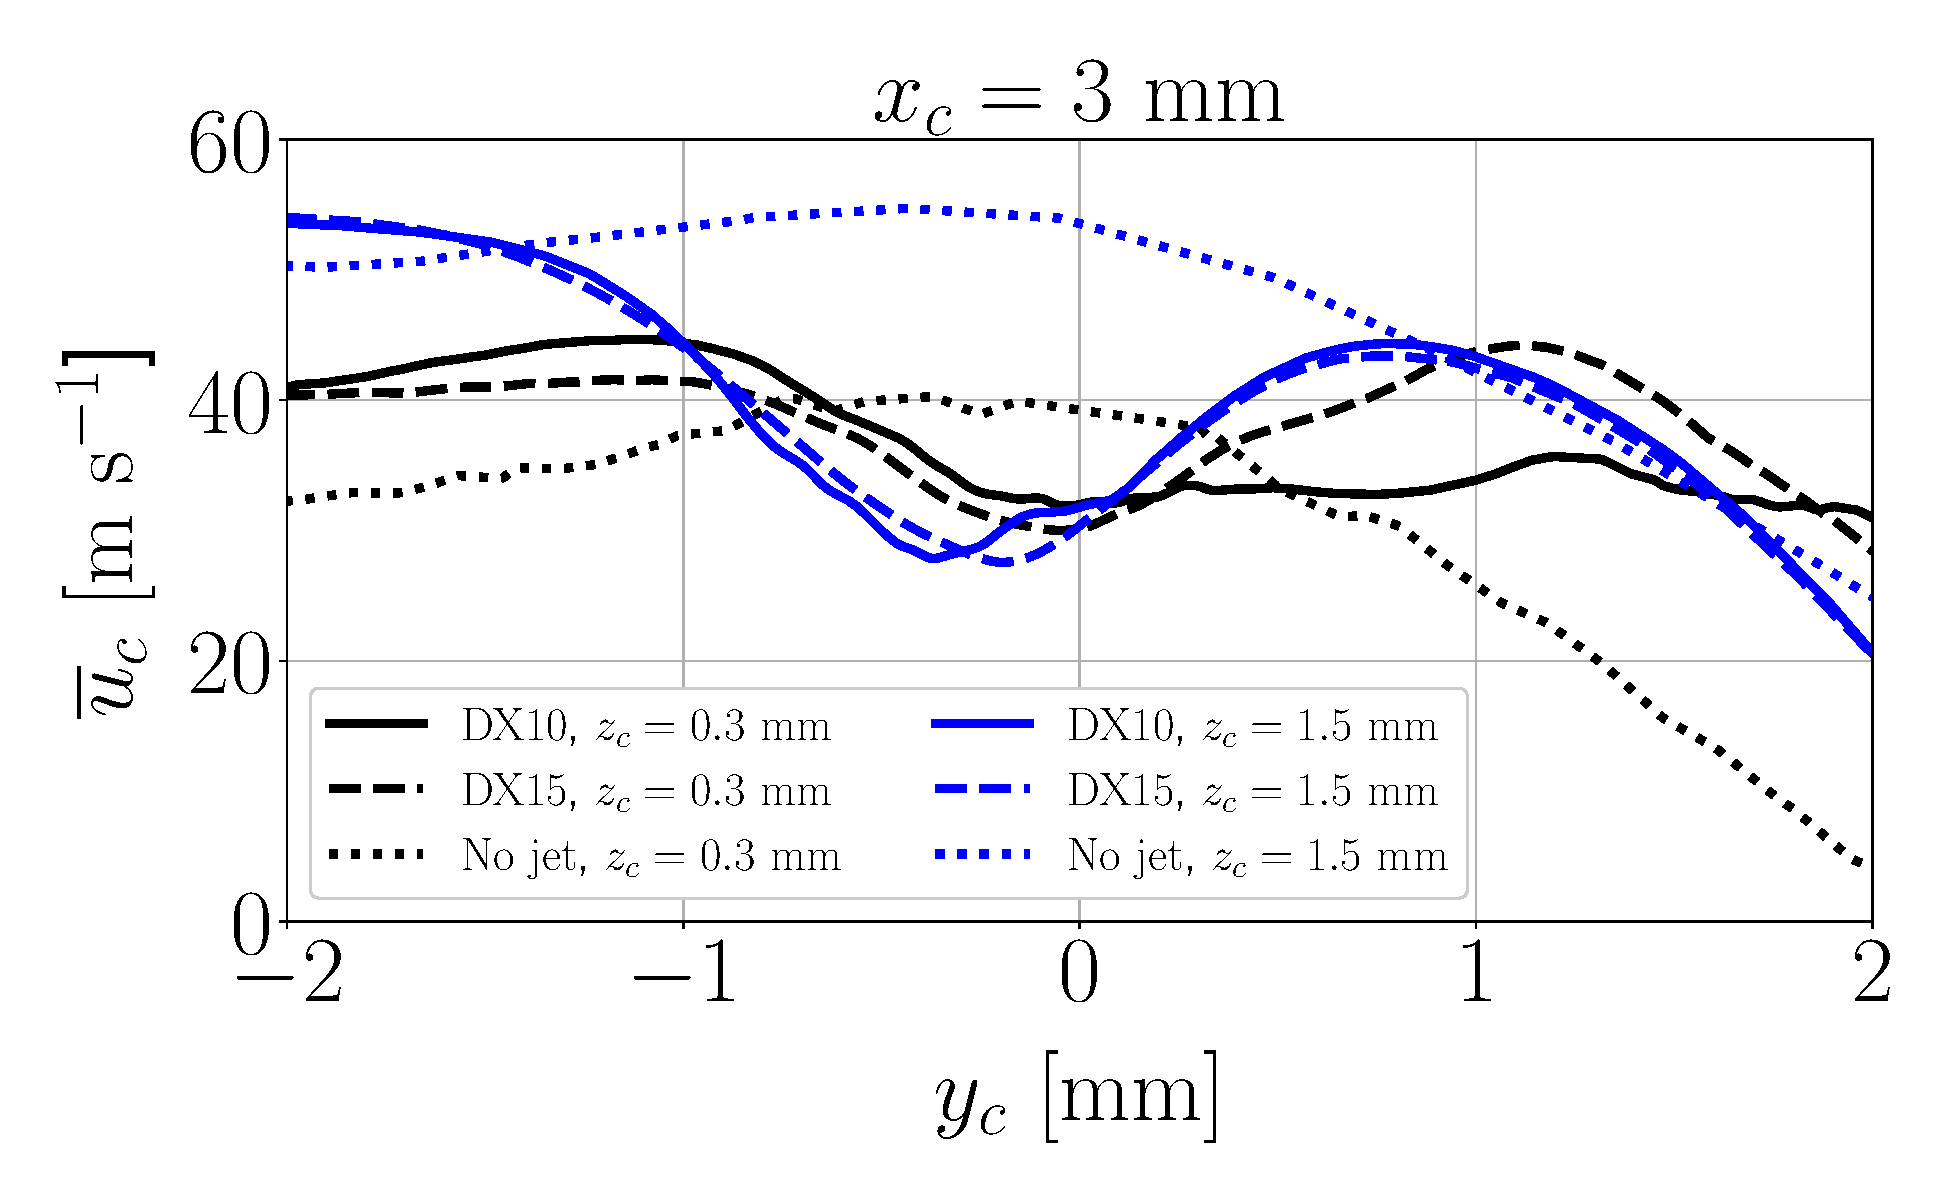
\includegraphics[scale=0.24]{./part3_applications/figures_ch8_resolved/turbulent_structures/lines_iso_x_along_y_plane_x03mm}
   %\vspace*{-0.1in}
\end{subfigure}
   \caption[{Mean axial velocity evolution along lateral coordinate at $z_c$ lines of Figure \ref{fig:BIMER_turbulent_structures_planes_z}}]{Mean axial velocity evolution along lateral coordinate at $z_c$ lines of Figure \ref{fig:BIMER_turbulent_structures_planes_z}. Dotted circles englobe gaseous vortical structures}
\label{fig:BIMER_sps_lines_iso-x_along_y_ux_mean}
\end{figure}

Finally, the gaseous fields at planes perpendicular to the vertical direction $z_c$ are displayed in Figure \ref{fig:BIMER_turbulent_structures_planes_z}. The recirculation bubble is observed close to the wall $z_c = 0.15$ mm for both cases, and further away ($z = 0.6$ mm) for case DX15 only, while case DX10 at $z = 0.6$ mm shows a high deceleration of the flow which does not reach recirculation. The deceleration fields are symmetric with respect to $y_c = 0$ closer to the wall but asymmetric further away from it: near-wall the freestream velocity is smaller in absolute value since it is within the boundary layer, hence the swirl effect is weaked and the gaseous field is less deviation, resulting in symmetry. Further away from the wall, the freestream is larger and the swirl effects are stronger, hence creating asymmetry. Similar observations have been obtained experimentally in gaseous jets in crossflow where swirl has been imposed to the gaseous phase \citepColor[panda_structure_2015].



\begin{figure}[ht]
\centering
   \includeinkscape[inkscapelatex=false,scale=0.18]{./part3_applications/figures_ch8_resolved/turbulent_structures/planes_z_ux_mean}
\caption[Mean axial velocity at planes $z = 0.2, 0.8, 16$ mm]{Mean axial velocity at planes $z = 0.2, 0.8, 16$. Black lines with arrows are in-plane mean streamlines. ; the white solid line indicates the contour $\overline{u} = 0$ which delimites the recirculation bubble. The grey area  indicates the mean liquid region, identifed as $\overline{\psi} > 0.5$. The black-dotted circle indicates the location of the injection nozzle}
\label{fig:BIMER_turbulent_structures_planes_z}
\end{figure}



\section{Direct measurement of liquid fluxes}
\label{sec:ch8_BIMER_IBs}

Resolved liquid fluxes are obtained in  interior boundaries (IBs) defined at the same location as the sampling planes from Figure \ref{fig:BIMER_local_FoR_and_sampling_planes}. The procedure followed to obtaine these fluxes was described in $\S$\ref{subsec:ch5_interior_boundaries}. Filming planes are not quantified in this case, since these fluxes are not used by the SLI models and it was shown ($\S$\ref{subsec:ch5_mass_conservation_ACLS_set_levelset_band}) that not all the mass losses in the planes perpendicular to the crossflow direction were due to liquid filming, but also to liquid structures reaching a characteristic size of the order of the mesh resolution.




\begin{figure}[ht]
	\centering
   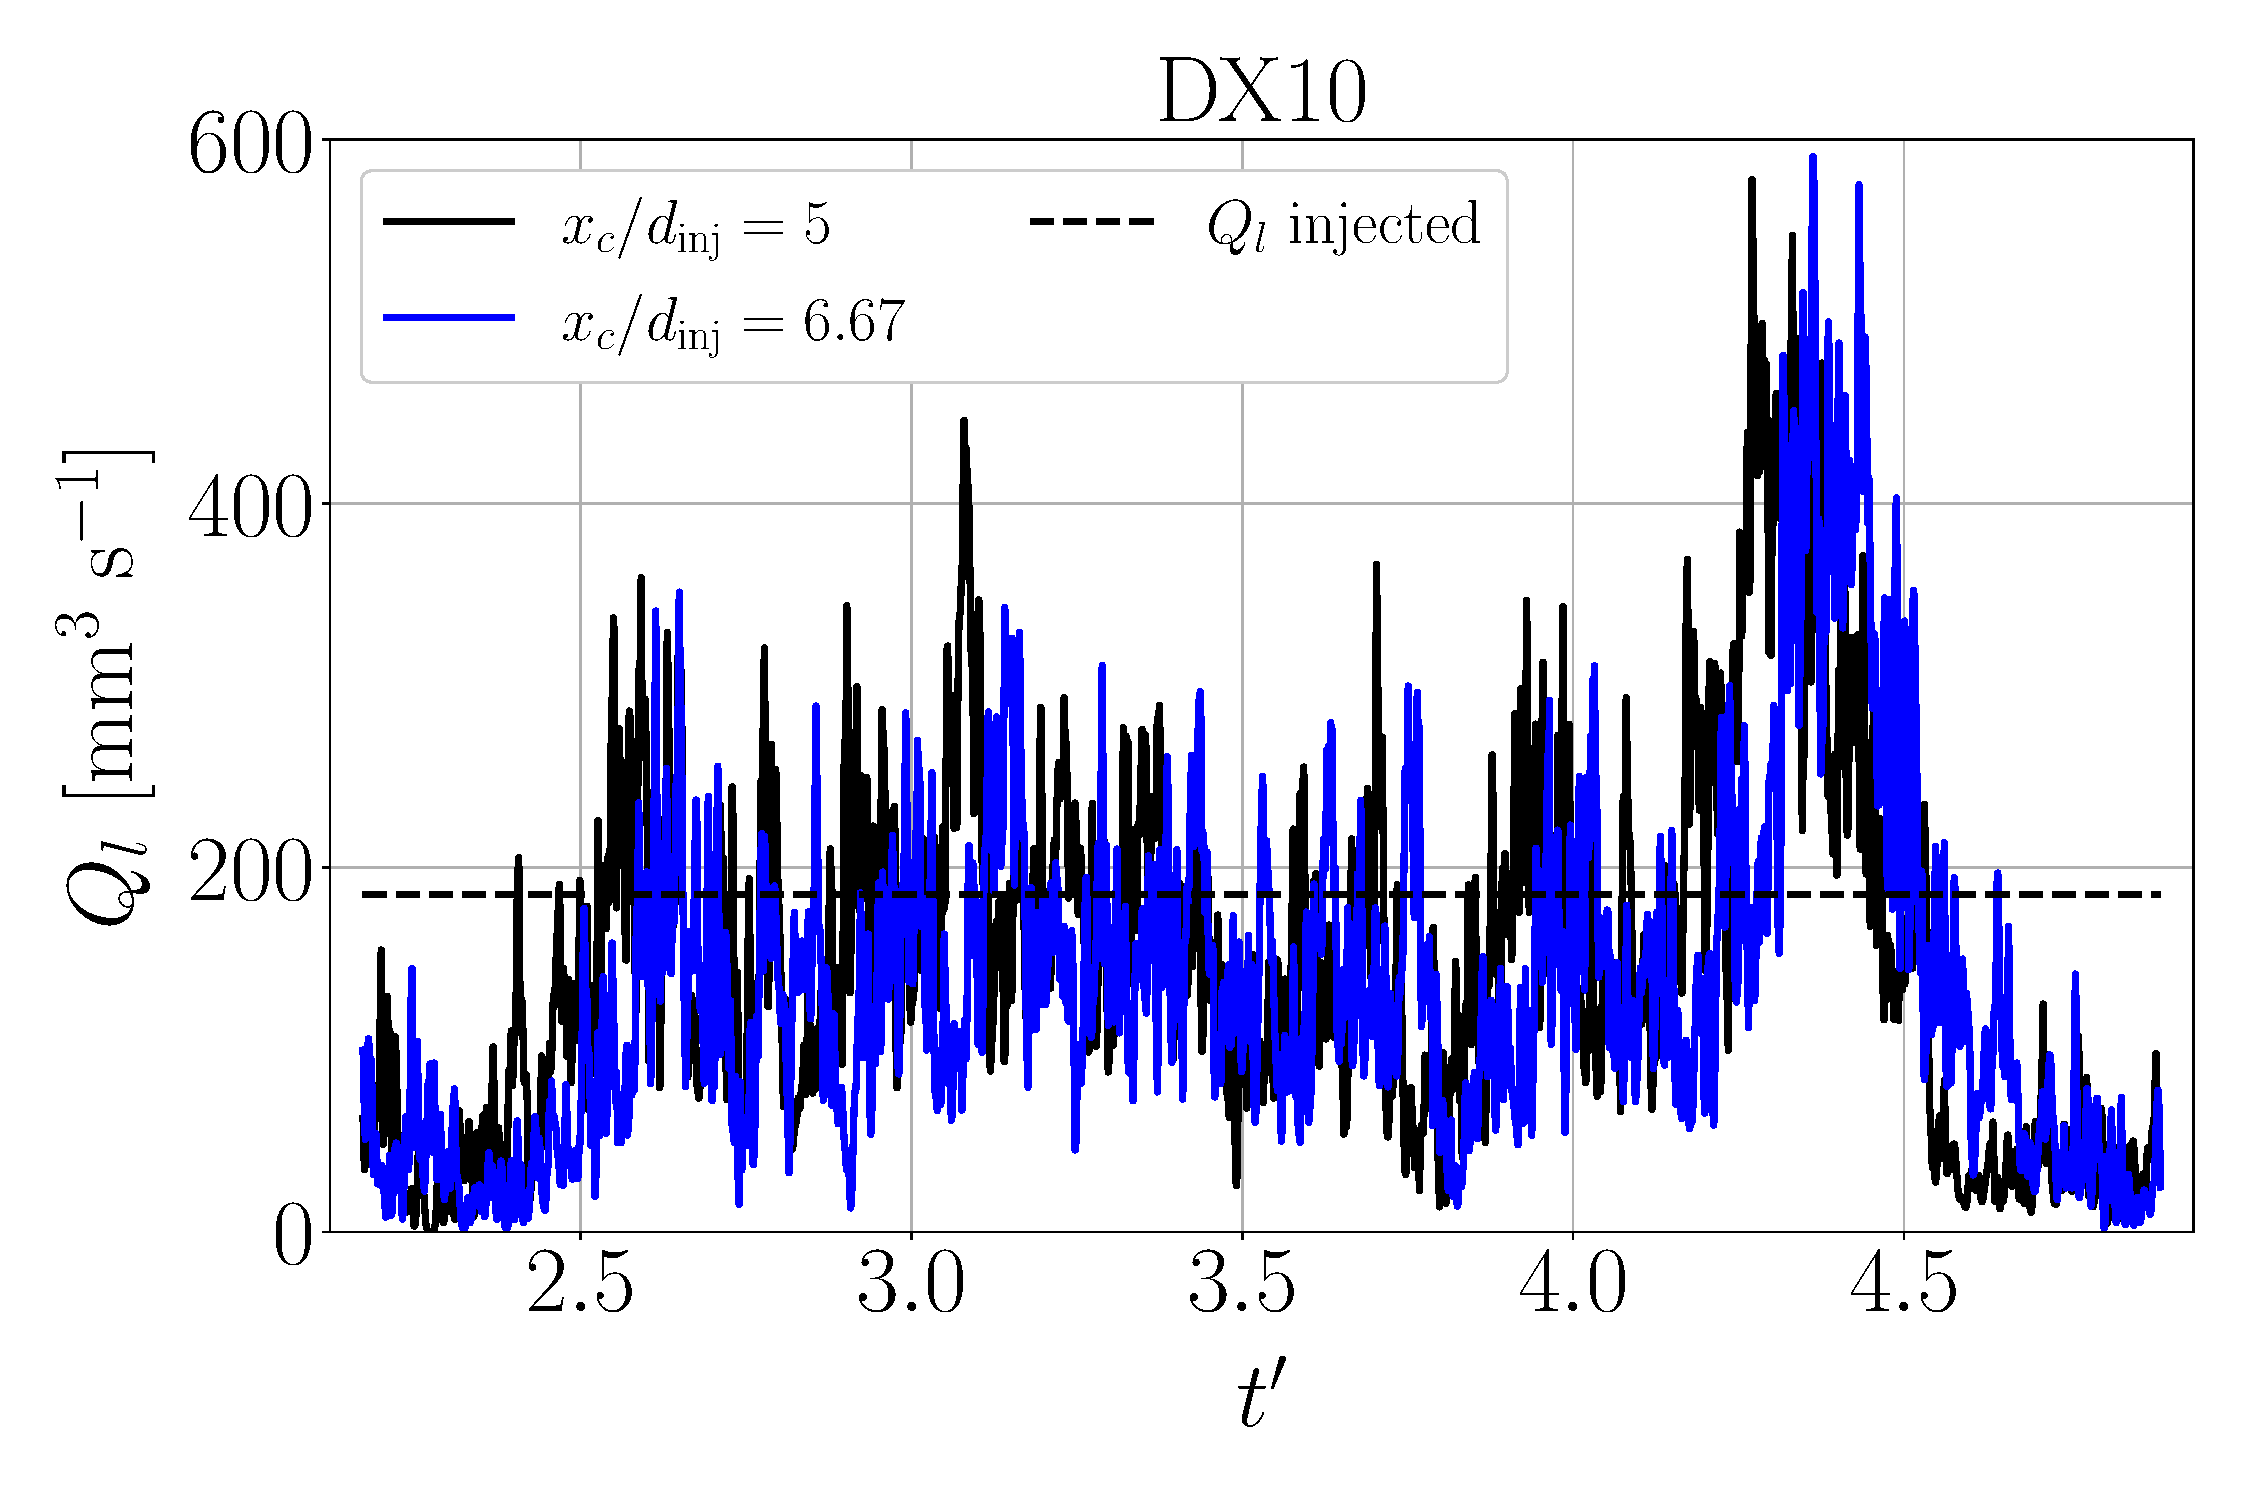
\includegraphics[scale=0.222]{./part3_applications/figures_ch8_resolved/flow_rates_ibs/inst_Q_iso_x_DX10}
   \vspace*{-0.20in}
\caption{Time evolution of instantaneous liquid flow rates $Q_l$ for case DX10}
\label{fig:IB_liquid_flow_rate_inst_evolution_BIMER}
\end{figure}

\clearpage

In first place, the instantaneous flux for simulation DX10 are shown in Figure \ref{fig:IB_liquid_flow_rate_inst_evolution_BIMER} for two sampling planes. In the same way as in the classical JICF (Figure \ref{fig:IB_liquid_flow_rate_inst_evolution_UG100_DX10}), the instantaneous fluxes show high oscillations around the injected flow rate due to the intermittent behaviour of the JICF: at certain instants there are cluster of droplets produced by the column breakup mechanism (see $\S$\ref{ch8:subsec_BIMER_breakup_topology}) crossing the sampling planes together, which yield instantaneous flux values larger than the injected $Q_l$ (flux overshoots); while at other instants there are only a few droplets being convected.


The evolution of the mean ($\overline{Q}_l$) and RMS ($Q_\mathrm{l,\mathrm{RMS}}$) flow rates through the IBS for all simulations is shown in Figure \ref{fig:IB_mean_RMS_Ql_evolution}. Mean fluxes (Figure \ref{fig:IB_mean_RMS_Ql_evolution} left) show oscillations at the early instants and a later stabilization to converged values. Case DX15 is converged while case DX10 shows still oscillations at the last sampling times due to the flux overshoots around $t^\prime \sim 4.2$ shown in Figure \ref{fig:IB_liquid_flow_rate_inst_evolution_BIMER}. Such overshoots are also reflected in the step increase in the RMS evolution (Figure \ref{fig:IB_mean_RMS_Ql_evolution} right) for the same case. %\hl{The coarses case DX15 shows the mean flux at the location $x_c/d_\mathrm{inj} = 0.33$, which is the closest location to the injector, to be larger than the injected mass flow rate: this is due to liquid flow recirculation at this location, since the resolution is coarse and the liquid structures emanating from the dense core stay attached to it... This recirculation has not been observed for the other two resolutions, which indicates that the interface resolution $\Delta x_\mathrm{min} = 15~\mu $m is not enough to resolve BIMER}.

In all simulations, there is a decrease in the mass flux with increasing axial distance $x_c$ as it was also observed in the JICF simulations of Chapter \ref{ch5:jicf_resolved_simulations}. The final mean values of the fluxes, displayed in the bar chart of Figure \ref{fig:BIMER_IB_bargraph_mean}, reflect this trend of mass flux reduction in a more visual way. The RMS values are also shown in the same graph by the vertical bars: these ones have large magnitudes, of the order of the mass flow rates obtained (see Figure \ref{fig:IB_mean_RMS_Ql_evolution}b), which indicate the high variance in the instantaneous mass flow rates crossing the sampling planes. Regarding fluxes decreases with axial distance, it is seen that the losses among consecutive samploing planes are larger for the coarse case DX15 than for the fine one DX10, since in the former the resolution limit is more restrictive and there are more droplets disappearing than in the latter. Even so, the mean fluxes show a good evolution with values close to the injected flow rates, with reductions along the axial distance due to filming and vanishing liquid structures when reaching a size of the order of the mesh resolution, as it was demonstrated in the resolved simualtions of the JICF test case from Chapter \ref{ch5:jicf_resolved_simulations}.

%\begin{figure}[ht]
%\centering
%   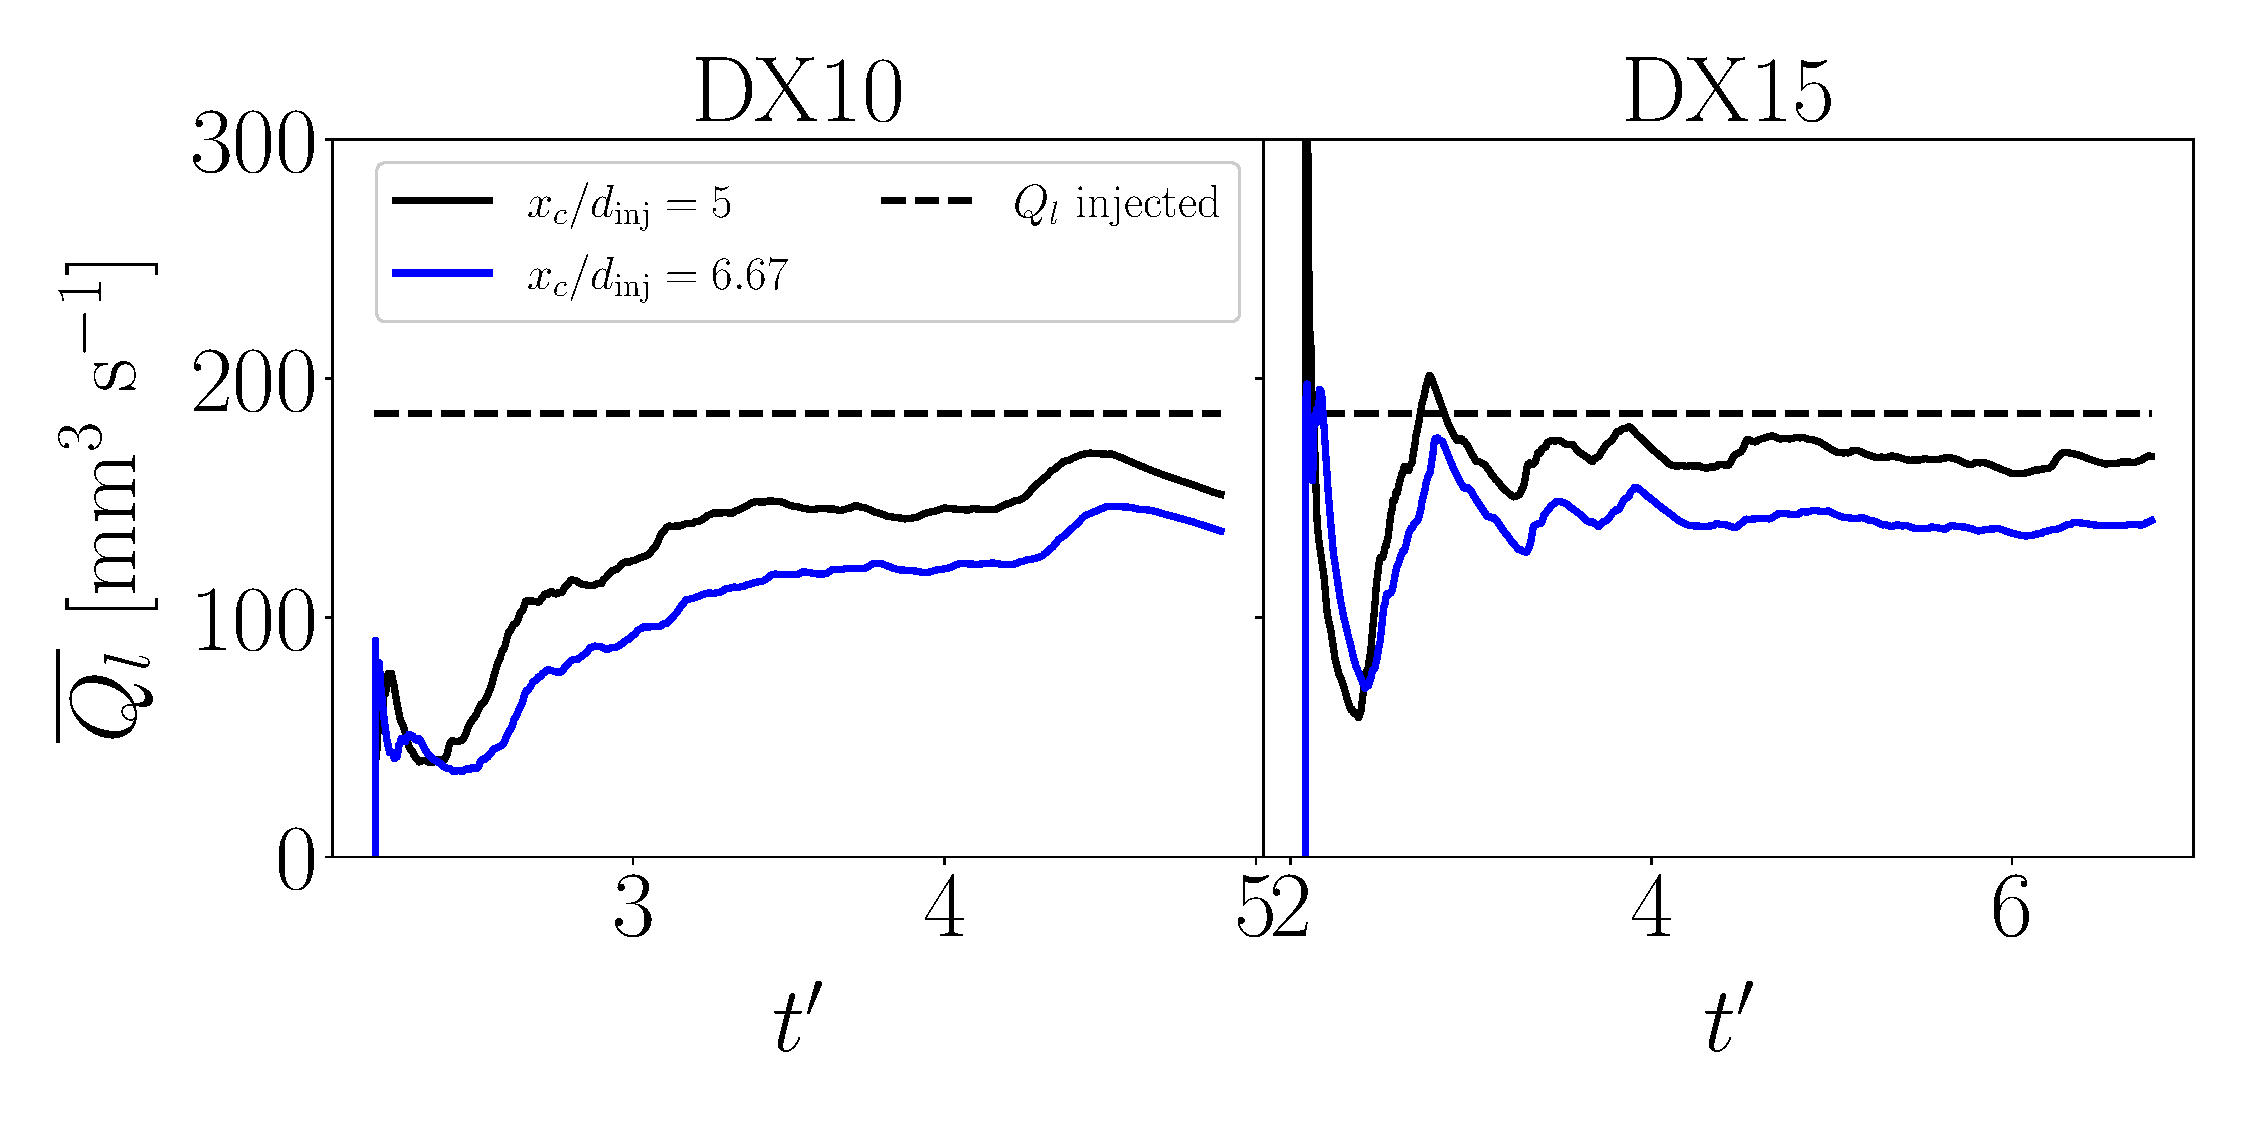
\includegraphics[width=0.48\textwidth]{./part3_applications/figures_ch8_resolved/flow_rates_ibs/evolution_mean_Q_iso_x}
%   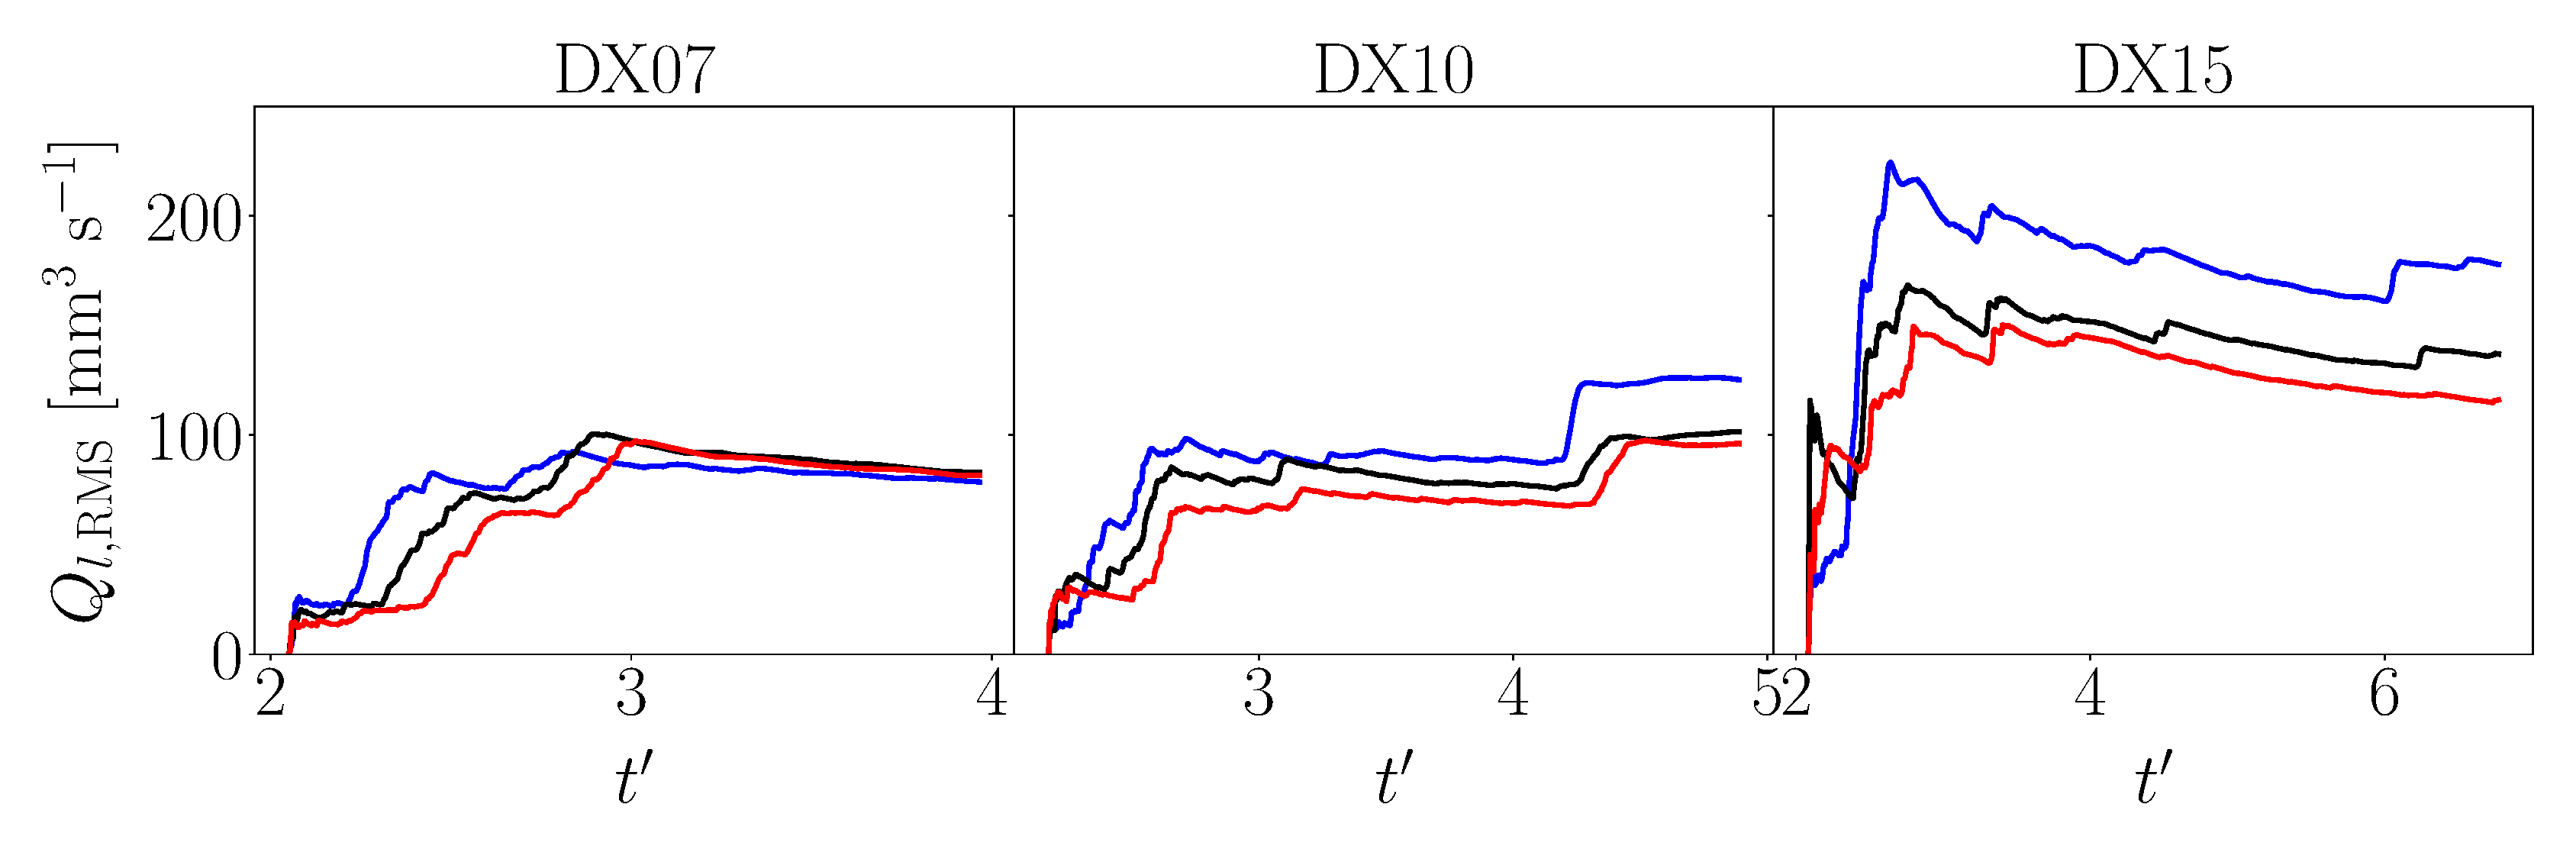
\includegraphics[width=0.48\textwidth]{./part3_applications/figures_ch8_resolved/flow_rates_ibs/evolution_RMS_Q_iso_x}
%   \caption{Mean (\textsl{left}) and RMS (\textsl{right}) $Q_l$ evolution in IBs perpendicular to crossflow.}
%\label{fig:IB_mean_RMS_Ql_evolution}
%\end{figure}

\begin{figure}[ht]
\centering
\begin{subfigure}[b]{0.9\textwidth}
	\centering
   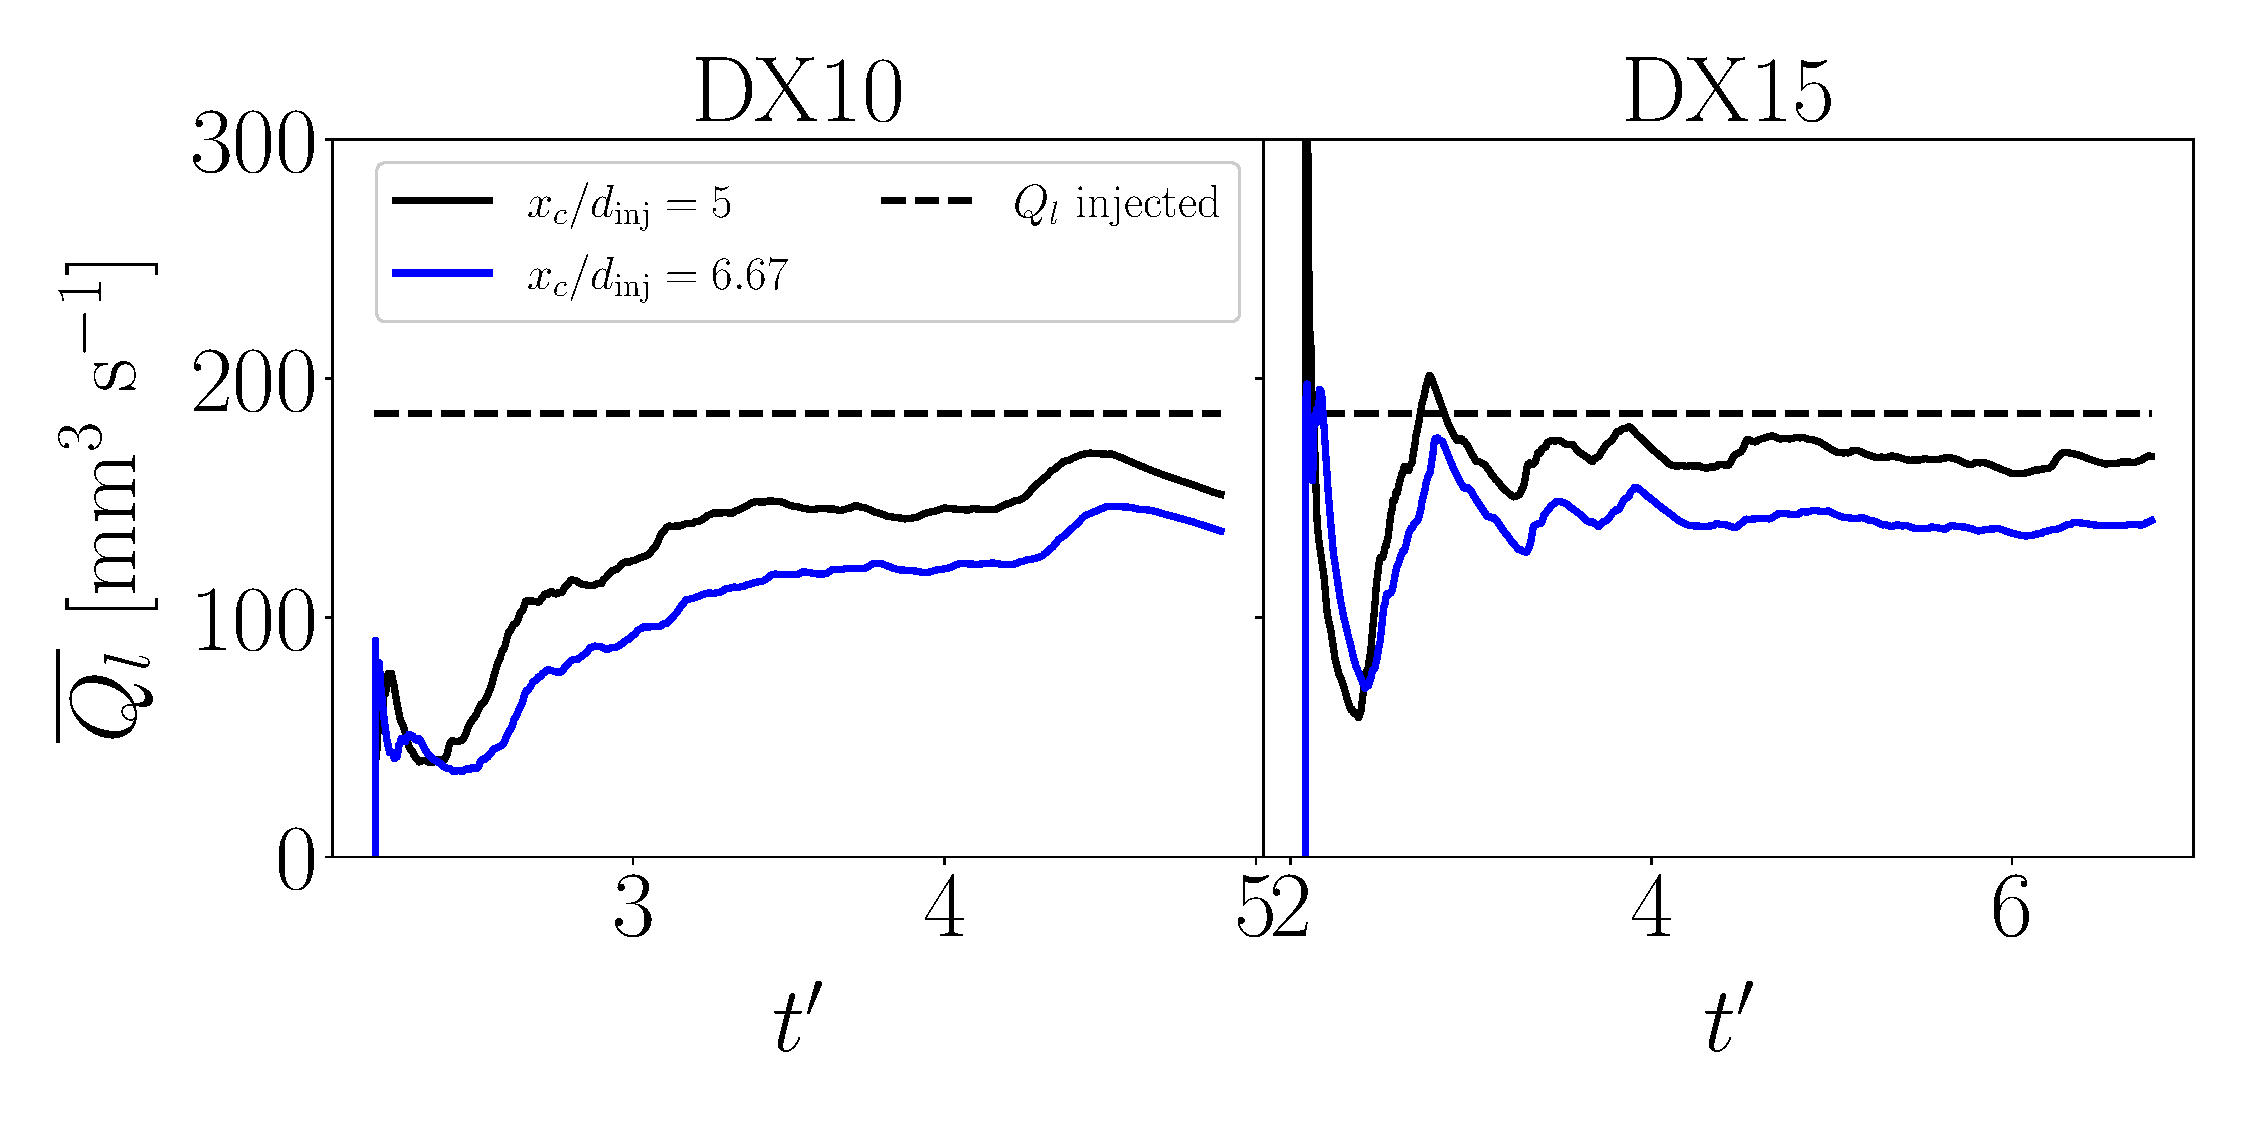
\includegraphics[scale=0.3]{./part3_applications/figures_ch8_resolved/flow_rates_ibs/evolution_mean_Q_iso_x}
   \vspace*{-0.15in}
   %\caption{Mean $Q_l$ evolution in IBs perpendicular to crossflow.}
   %\label{} 
\end{subfigure}
\vskip\baselineskip
\begin{subfigure}[b]{0.9\textwidth}
	\centering
   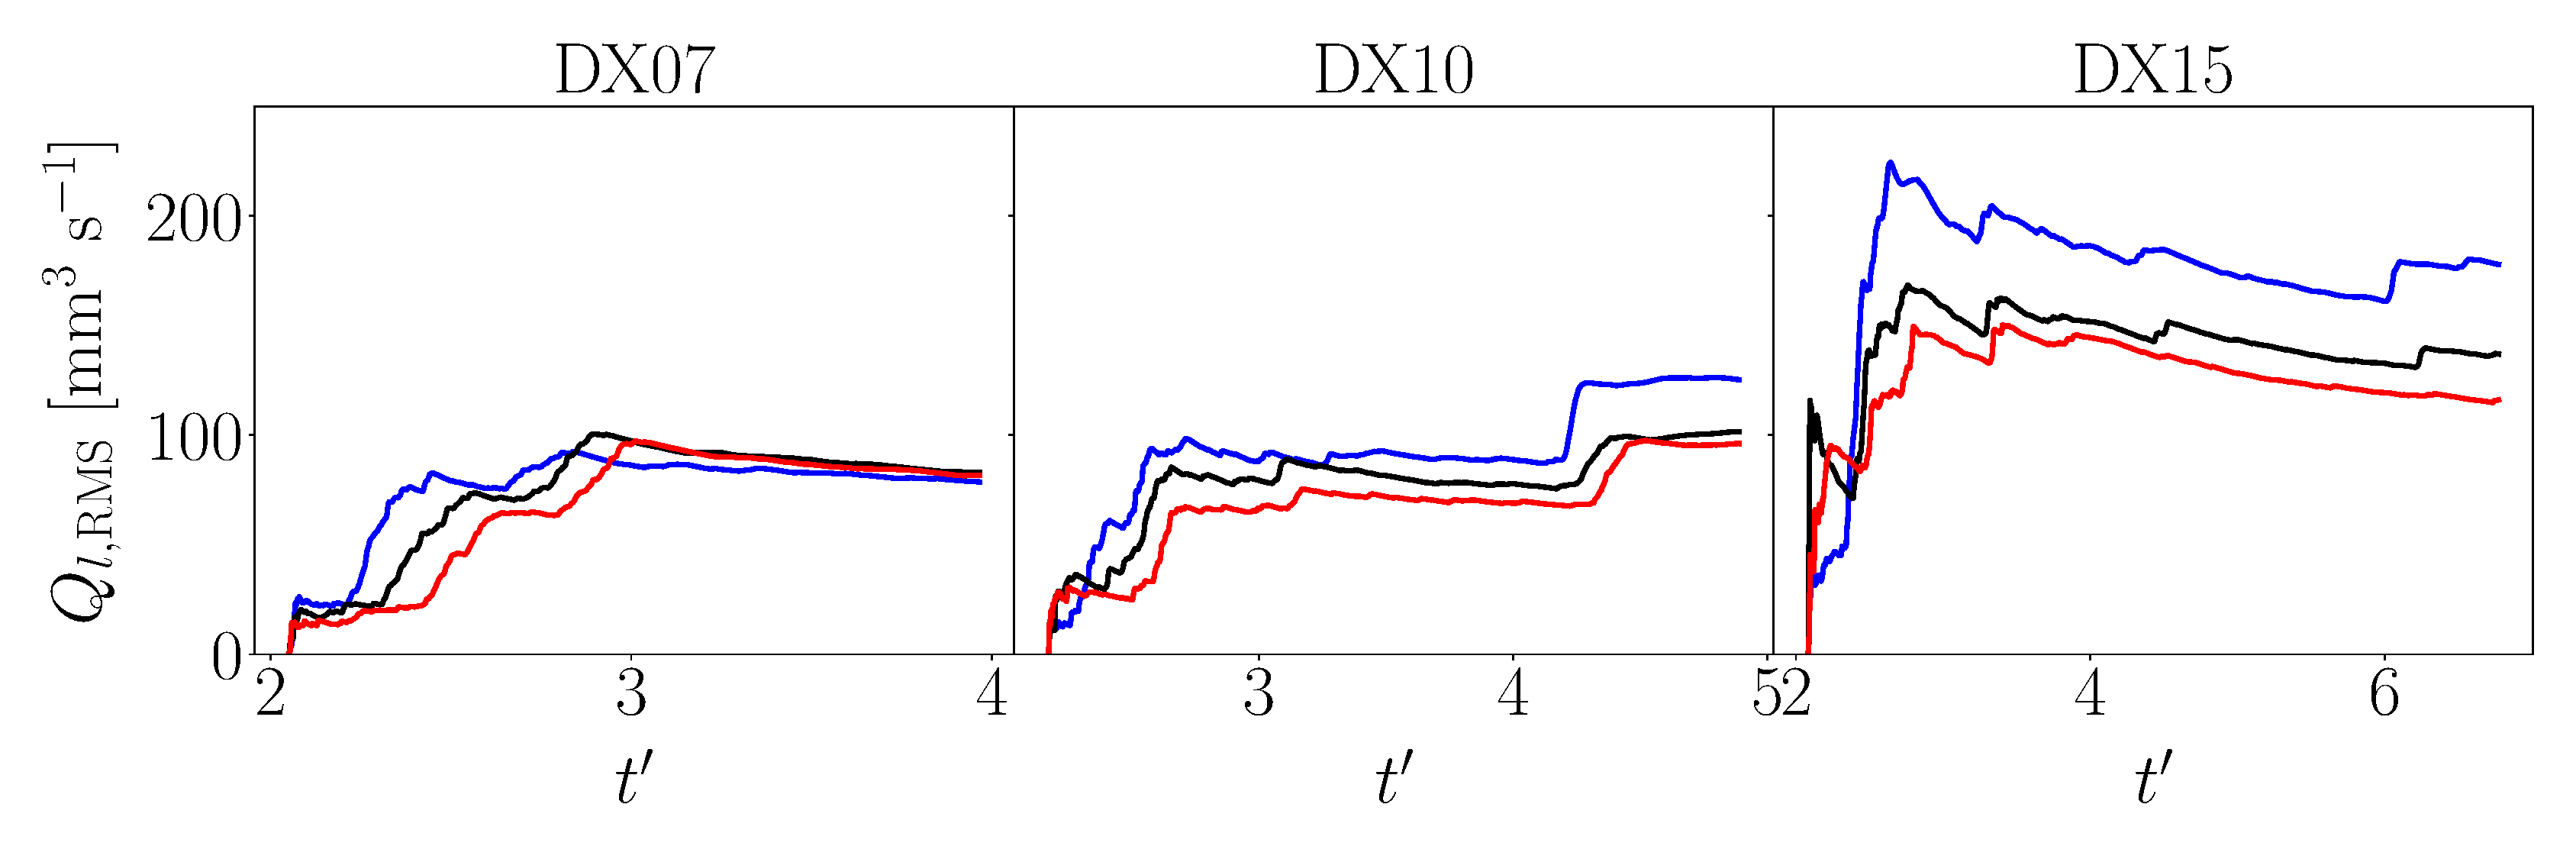
\includegraphics[scale=0.3]{./part3_applications/figures_ch8_resolved/flow_rates_ibs/evolution_RMS_Q_iso_x}
   \vspace*{-0.15in}
   %\caption{RMS $Q_l$ evolution in IBs perpendicular to crossflow.}
   %\label{}
\end{subfigure}
\caption{Time evolution of mean (\textsl{top}) and RMS (\textsl{bottom}) fluxes in BIMER IBs}
\label{fig:IB_mean_RMS_Ql_evolution}
\end{figure}

\clearpage




\begin{figure}[ht]
\centering
   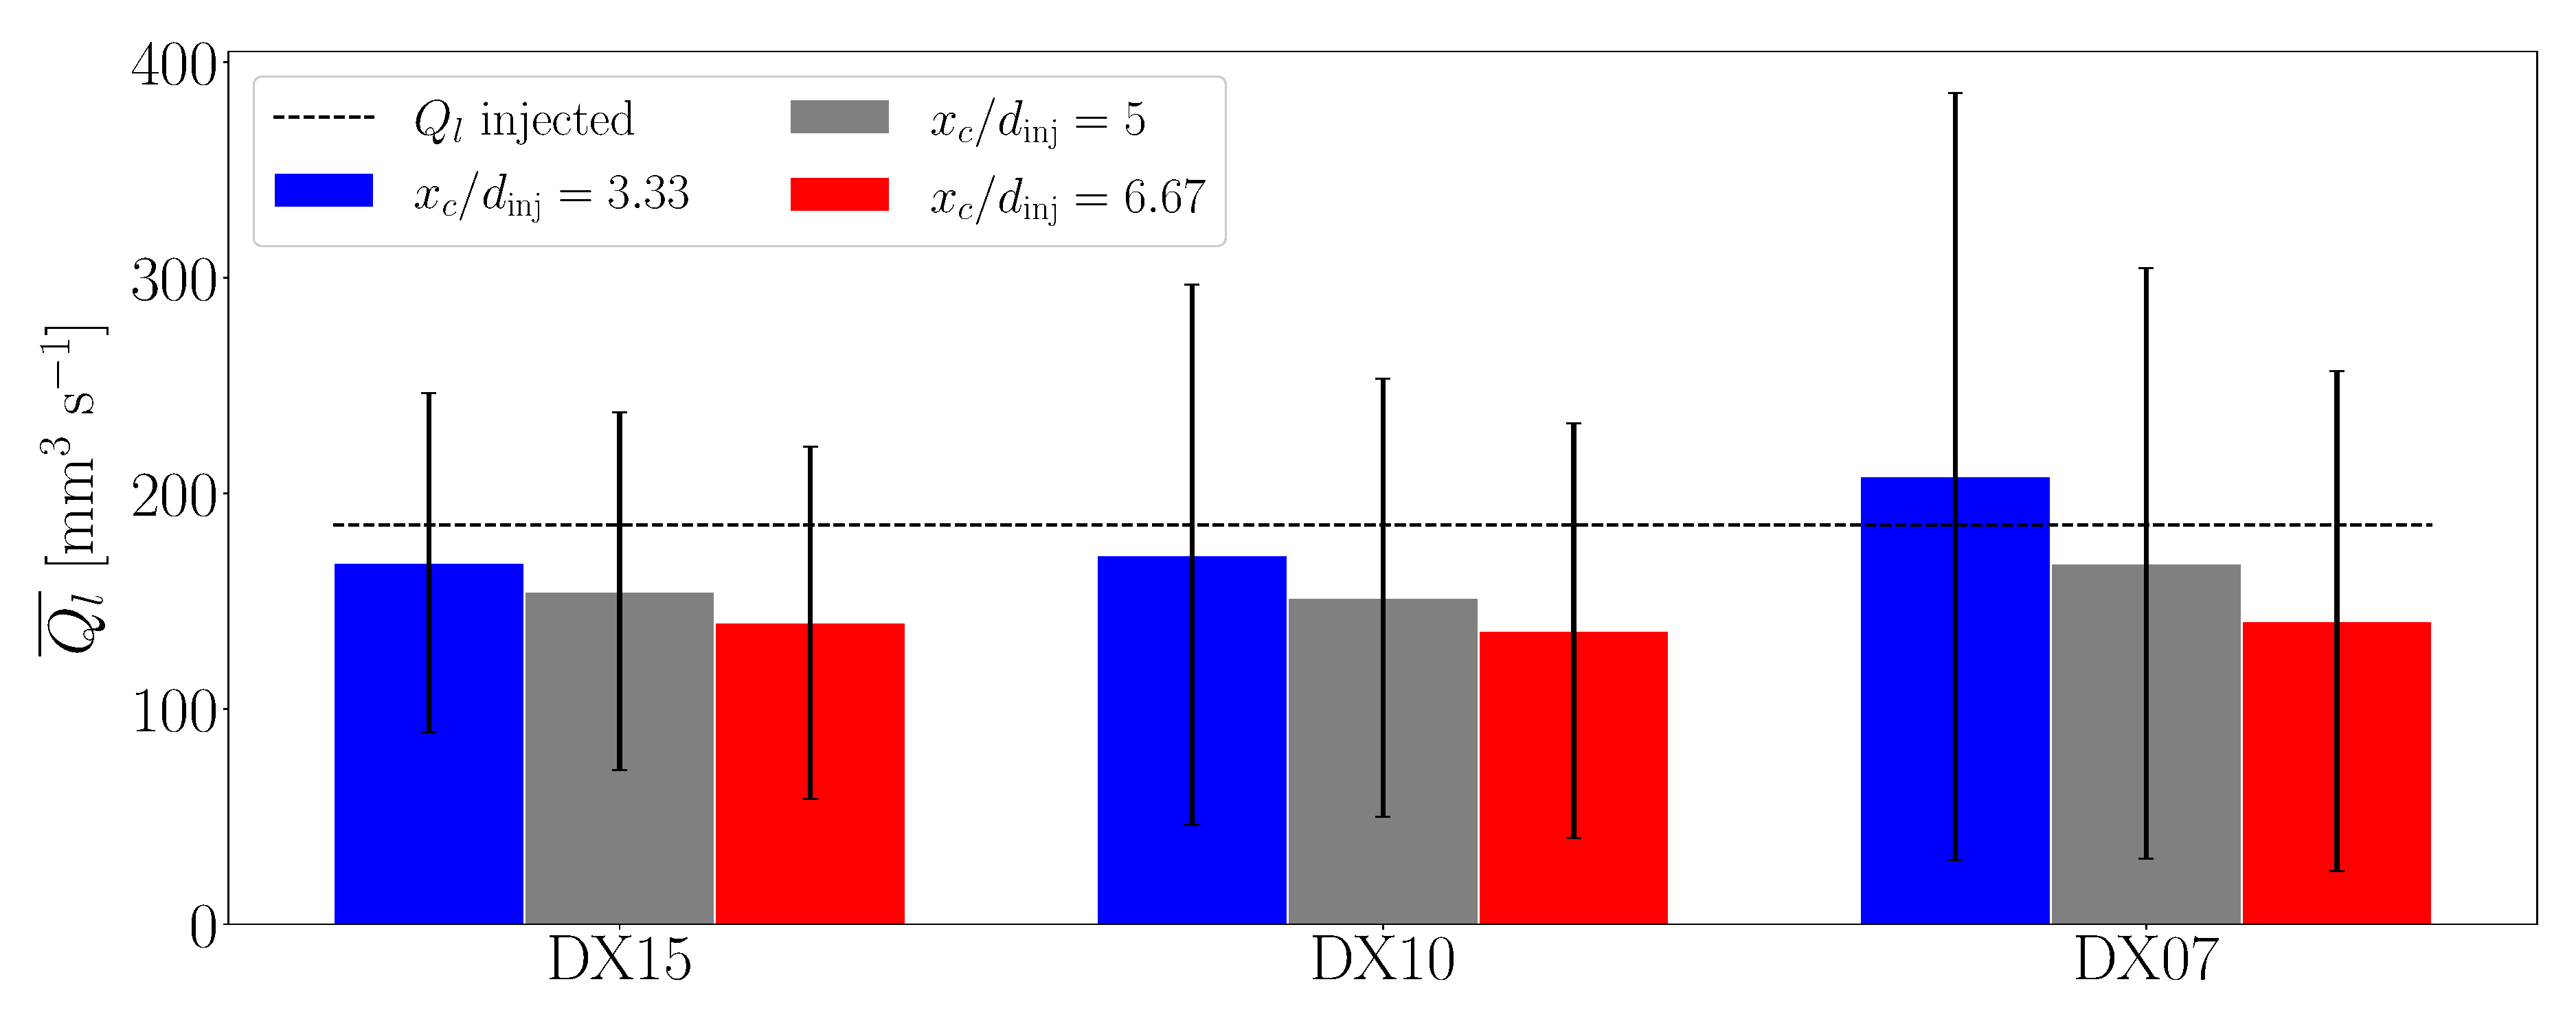
\includegraphics[scale=0.25]{./part3_applications/figures_ch8_resolved/flow_rates_ibs/bar_graph_isox_IBs}
\caption{Mean flow rates from IBs perpendicular to crossflow in BIMER}
\label{fig:BIMER_IB_bargraph_mean}
\end{figure}


\section{Spray characterization}
\label{sec:ch8_BIMER_spray_char}

\subsection{Establishment of mean sprays}

Characterization of the spray resulting from atomization in BIMER is obtained through lagrangian tracking of the resulting liquid structures when these cross the sampling planes. The sampling procedure and the droplets properties obtained were described in $\S$\ref{subsec:SLI_spray_sampling}. The total physical time simulated and time for which statistics and droplets have been accumulated (i.e. after an establishment time of $t^\prime \sim 2$) are summarized in Table \ref{tab:BIMER_SLI_t_prime_accumulation}.  The total number of droplets accumulated in all sampling planes from each simulation are shown in Tabl \ref{fig:ch8_spray_char_establishment}. Even though the total number of sampled= droplets is similar in all cases, it is clearly seen by looking at $N_\mathrm{dr}/t_\mathrm{acc}$ that the fine simulation generates more droplets, as more droplets are sampled per milisecond simulated. This is in line with the effect of the resolution in the JICF of Chapter \ref{ch5:jicf_resolved_simulations}, where the observations on the effect of resolution in the sampled sprays were identical (see Table \ref{tab:jicf_SLI_Ndr_accumulated}). 

%\begin{table}[!h]
%\centering
%\caption{Total accumulation times $t_\mathrm{acc}$  and $t_\mathrm{acc}^{\prime}$ (Eq. \ref{eq:t_prime_with_tau_drx10}) for each BIMER simulation}
%\begin{tabular}{ccc}
%\thickhline
% &  DX10 & DX15 \\
%\hline
%$t_\mathrm{ph}~[\mathrm{ms}]$ & 1.08 & 6.30 \\
%$t_\mathrm{ph}^{\prime}$ & 3.64 & 17.70 \\
%$t_\mathrm{acc}~[\mathrm{ms}]$ & 0.53 & 5.48 \\
%$t_\mathrm{acc}^{\prime}$ & 1.79& 15.40 \\
%\thickhline
%\end{tabular}
%\label{tab:BIMER_SLI_t_prime_accumulation}
%\end{table}

\begin{table}[!h]
\centering
\caption{Total physical $t_\mathrm{ph}$ and accumulation times $t_\mathrm{acc}$, absolute and dimensionless with Eq. (\ref{eq:t_prime_BIMER_with_tau_drx10}), for each BIMER simulation}
\begin{tabular}{ccccc}
\thickhline
\textbf{Case} &  $t_\mathrm{ph}~[\mathrm{ms}]$ & $t_\mathrm{ph}^{\prime}$ & $t_\mathrm{acc}~[\mathrm{ms}]$ & $t_\mathrm{acc}^{\prime}$ \\
\hline
DX10 & 1.73 & 4.89 & 0.96 & 2.72 \\
DX15 & 3.81 & 6.78 & 2.64 &  4.69 \\
\thickhline
\end{tabular}
\label{tab:BIMER_SLI_t_prime_accumulation}
\end{table}


%\begin{table}[!h]
%\centering
%\caption{Number of droplets sampled in BIMER simulations: total amount ($N_\mathrm{dr}$) and total amount per accumulation time $N_\mathrm{dr}/t_\mathrm{acc}$}
%\begin{tabular}{cccccc}
%\thickhline
%\multirow{2}{*}{ \textbf{Case}}  & \multicolumn{2}{c}{$N_\mathrm{dr}$} & & \multicolumn{2}{c}{$N_\mathrm{dr}/t_\mathrm{acc}~[\mathrm{ms}^{-1}]$} \\
%\cline{2-3} \cline{4-6}
%& $x/d_\mathrm{inj} = 5$ & $x/d_\mathrm{inj} = 3.33$ &  & $x/d_\mathrm{inj} = 5$ & $x/d_\mathrm{inj} = 3.33$  \\
%\thickhline 
%DX10  & 6214 & 5674 & & 6463 & 5901 \\
%DX15  & 6854 & 6112 & & 2598 & 2316 \\
%\thickhline
%\end{tabular}
%\label{tab:BIMER_SLI_Ndr_accumulated}
%\end{table}

%\begin{table}[!h]
%\centering
%\caption{Number of droplets sampled in BIMER simulations: total amount ($N_\mathrm{dr}$) and total amount per accumulation time $N_\mathrm{dr}/t_\mathrm{acc}$}
%\begin{tabular}{cccccccccc}
%\thickhline
%\multirow{2}{*}{ \textbf{Case}}  & \multicolumn{4}{c}{$N_\mathrm{dr}$} & & \multicolumn{4}{c}{$N_\mathrm{dr}/t_\mathrm{acc}~[\mathrm{ms}^{-1}]$} \\
%\cline{2-5} \cline{7-10}
%& $x/d_\mathrm{inj} = 5$ & $6.67$ & $8.33$ & $10$ &  & $5$ & $6.67$ & $8.33$ & $10$  \\
%\thickhline 
%DX10  & 6214 & 5674 & 5183 & 4701 & & 6463 & 5901 & 5390 & 4889  \\
%DX15  & 6854 & 6112 & 5077 & 3945 &  & 2598 & 2316 & 1924 & 1495  \\
%\thickhline
%\end{tabular}
%\label{tab:BIMER_SLI_Ndr_accumulated}
%\end{table}

\begin{table}[!h]
\centering
\caption{Number of droplets sampled in BIMER simulations: total amount ($N_\mathrm{dr}$) and total amount per accumulation time $N_\mathrm{dr}/t_\mathrm{acc}$}
\begin{tabular}{cccccccccc}
\thickhline
\multirow{2}{*}{ \textbf{Case}}  & \multicolumn{4}{c}{$N_\mathrm{dr}$} & & \multicolumn{4}{c}{$N_\mathrm{dr}/t_\mathrm{acc}~[\mathrm{ms}^{-1}]$} \\
\cline{2-5} \cline{7-10}
& $x_c = 1.5~\mathrm{mm}$ & $2~\mathrm{mm}$ & $2.5~\mathrm{mm}$ & $3~\mathrm{mm}$ &  & $x_c = 1.5~\mathrm{mm}$ & $2~\mathrm{mm}$ & $2.5~\mathrm{mm}$ & $3~\mathrm{mm}$   \\
\thickhline 
DX10  & 6214 & 5674 & 5183 & 4701 & & 6463 & 5901 & 5390 & 4889  \\
DX15  & 6854 & 6112 & 5077 & 3945 &  & 2598 & 2316 & 1924 & 1495  \\
\thickhline
\end{tabular}
\label{tab:BIMER_SLI_Ndr_accumulated}
\end{table}



Establishment of the global spray in terms of flux $Q_l$ and $SMD$ is shown in Figure \ref{fig:ch8_spray_char_establishment}.  Flux evolution in all planes show similar trends as the IBs flow rates from Figure \ref{fig:BIMER_IB_bargraph_mean}, including a decrease in mean fluxes with axial distance due to liquid structures reaching the mesh resolution and disappearing. The evolution of SMD shows good convergence for all cases for the times simulated. The evolution of other mean quantities which are of interest for SLI are shown in Appendix \ref{app:BIMER_SLI_convergence}.


\begin{figure}[ht]
	\centering
   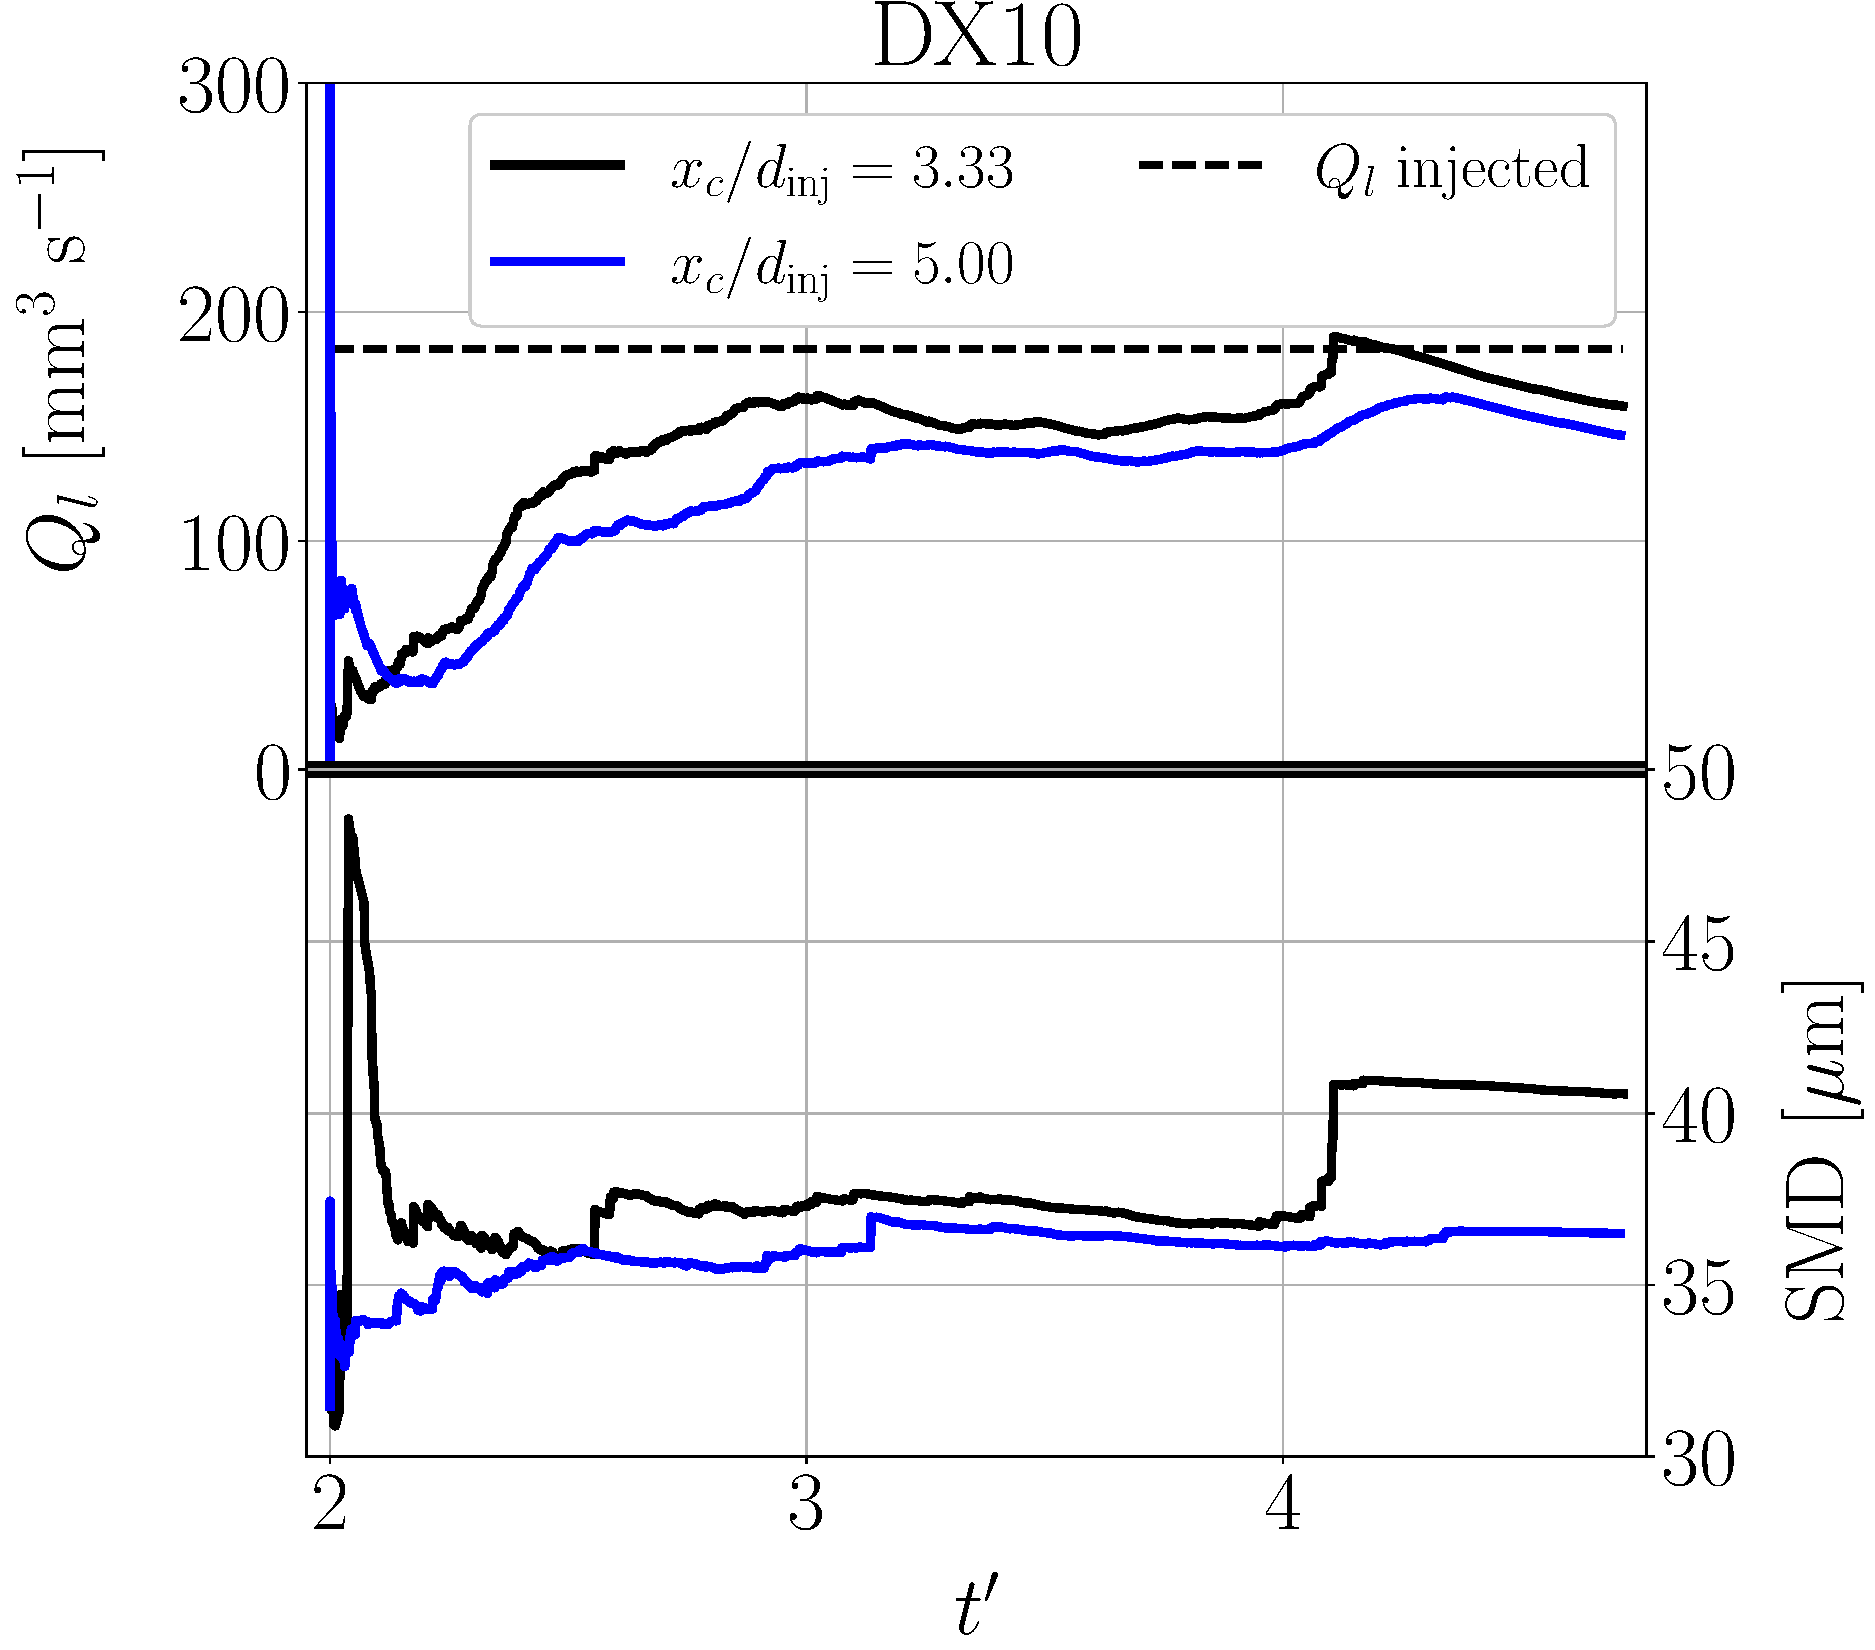
\includegraphics[width=0.45\textwidth]{./part3_applications/figures_ch8_resolved/SPRAY_characterization/establishment_and_fluxes/establishment_DX10}
   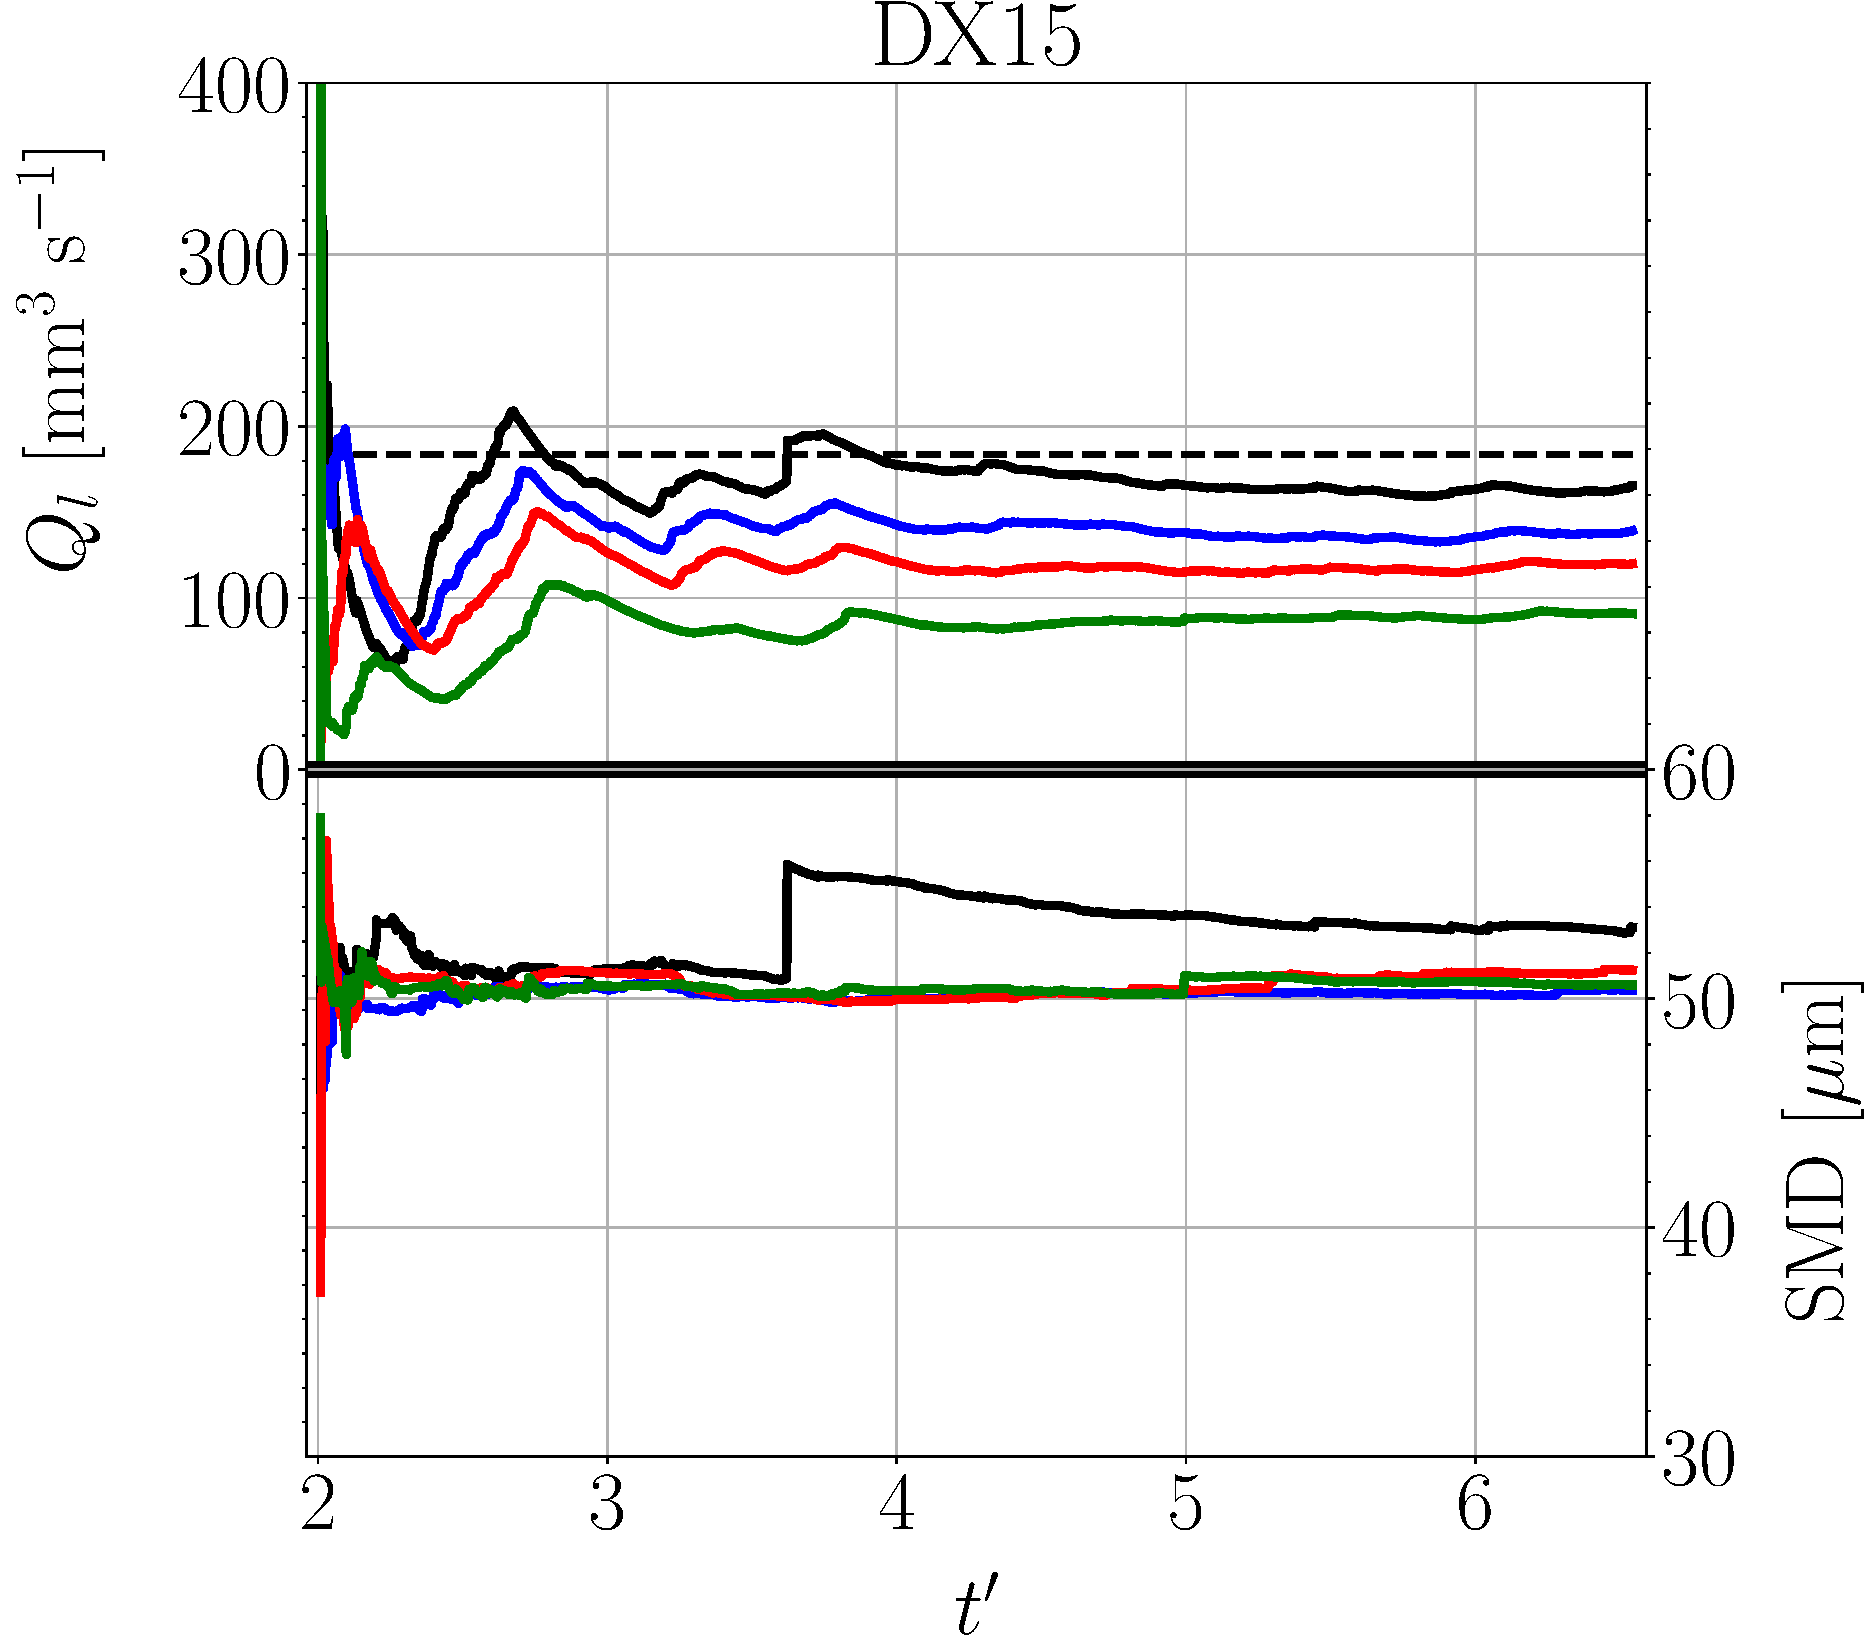
\includegraphics[width=0.45\textwidth]{./part3_applications/figures_ch8_resolved/SPRAY_characterization/establishment_and_fluxes/establishment_DX15}
   \caption{Establishment of SMD and $Q_l$ in BIMER sprays}
\label{fig:ch8_spray_char_establishment}
\end{figure}

\subsection{Liquid fluxes: lagrangian versus resolved}

The final fluxes obtained through lagrangian tracking are compared to their equivalent from the IBs in the barchart from Figure \ref{fig:ch8_fluxes_bargraph_IBs_vs_LGS}. As in the previous JICF studies (Figure \ref{fig:fluxes_bargraph_IBs_vs_LGS}), there are disparities among both methodologies to obtain fluxes: sometimes the lagrangian fluxes overestimate the IBs ones due to droplets being tracked more than once, while in other cases some droplets might not be detected at all through the lagrangian method and hence the fluxes are underestimated (more details are found in $\S$\ref{subsec:ch5_sli_fluxes_vs_IBs}). Overall, lagrangian fluxes are in the same order as the resolved ones, hence these ones are kept to represent the spray (later on, spatially discretized fluxes to be injected in the dispersed phase simulations from Chapter \ref{ch9:BIMER_lagrangian} will be scaled to match the real flux injected in BIMER).




%\subsection{Liquid fluxes: lagrangian versus resolved}
%\label{subsec:ch8_sli_fluxes_vs_IBs}



\begin{figure}[ht]
	\centering
   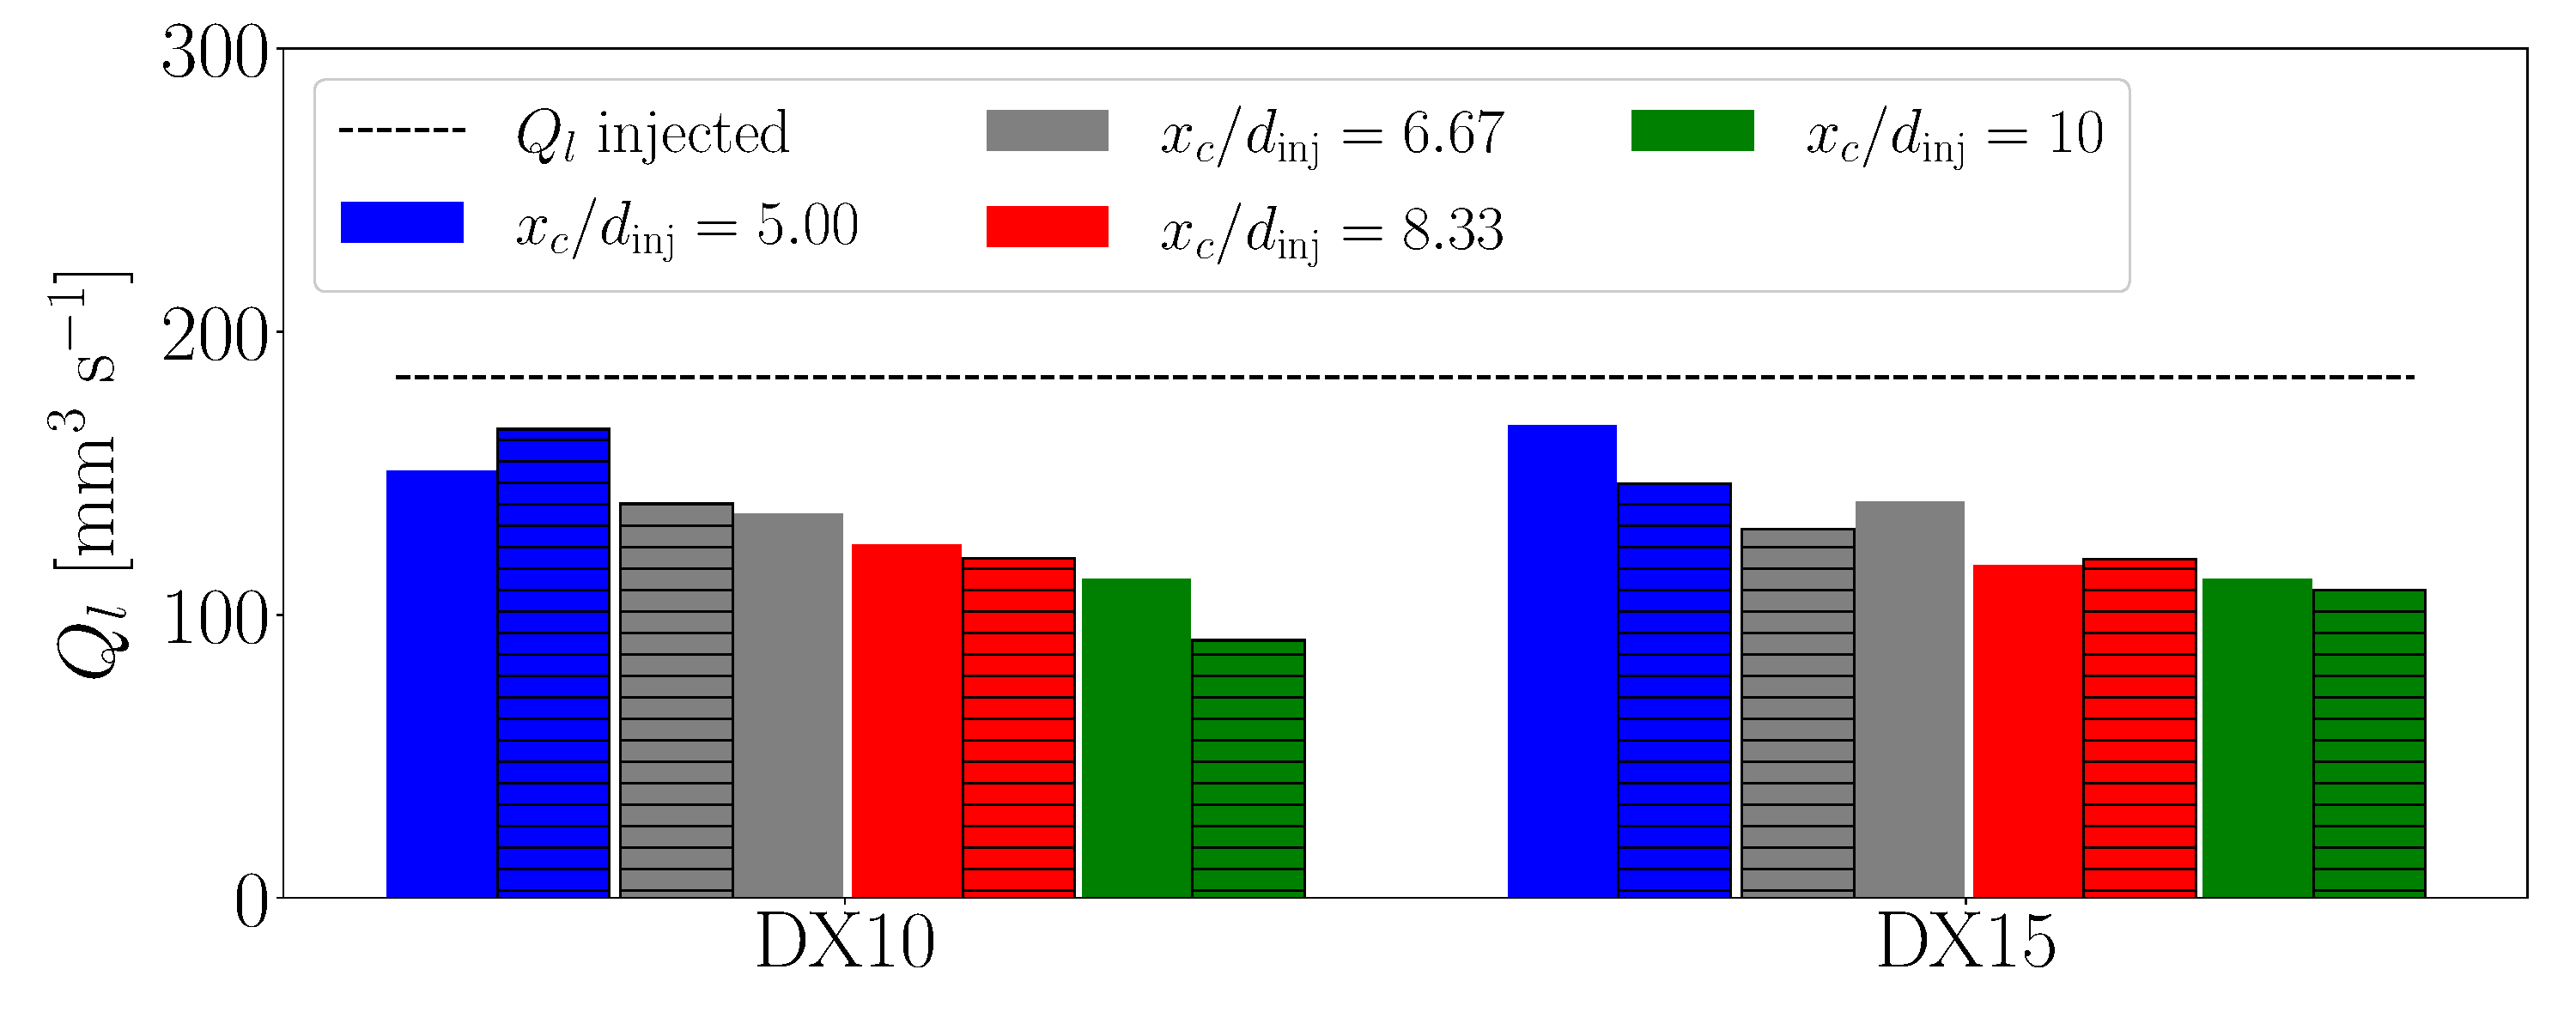
\includegraphics[scale=0.25]{./part3_applications/figures_ch8_resolved/SPRAY_characterization/establishment_and_fluxes/fluxes_SLI_vs_IBs}
   \caption{Liquid fluxes provided by interior boundaries (solid color bars) and lagrangian tracking (black-dashed color bars).}
   \label{fig:ch8_fluxes_bargraph_IBs_vs_LGS}
\end{figure}


\subsection{Granulometry}
\label{ch8:subsec_spray_char_granulo}

The final SMDs obtained are shown in Figure \ref{fig:ch8_spray_char_SMD_final}. The SMD has a clear dependency on the resolution: reducing the interface cell size $\Delta x_\mathrm{min}$ from 15 to 10 $\mu$m (1.5 factor) reduces the SMD from $\sim$ 50 to $\sim$ 35 $\mu$m, which is a reduction of the same order. SMD decreases with axial distance for both simulations. This variation is larger for DX15, where SMD decreases from 53 to 50 $\mu$m, than in DX10, where the reduction if from 36 to 35 $\mu$m. The variations are very low for both cases, indicating that either 1) the mesh resolution limit is reached or 2) atomization is complete and the smallest droplets can be captured with the interface resolutions employed. To assess both hypothesis it is of interest to look at the droplets size histograms in Figure \ref{fig:ch8_jicf_size_volume_histograms_all}.  The size and volume distributions are shown, as well as relevant sizes and the lognormal distributions (Eq. \ref{eq:ch5_f0_lognormal_distr_expression}) where the parameters have been obtained either by fit or through the correlations given by Eq. (\ref{eq:lefevbre_lognormal_fit_expressions}). The histograms from the coarse case DX15 show a clear lognormal distribution which is well fit by the blue curve. The smallest droplets sampled have a diameter $\sim 30~\mu$m, which corresponds to $2\Delta x_\mathrm{min}$. This means that the smallest droplets in the simulation are resolved with 2 mesh cells: in general, the number of cells to properly resolved a droplet is a subject of discussion, but authors agree generally that it is comprised between 2 \citepColor[herrmann_detailed_2009] and 5 \citepColor[fuster_simulation_2009]. Therefore, in the case DX15 where smallest droplets are $2\Delta x_\mathrm{min} = 30~\mu$m the smallest droplets simulated are limited by the grid, meaning that a finer resolution would be needed to resolve the smallest physical droplets that would exist in the actual configuration (unfortunately, there are no experimental data available to compare). When refining the mesh from $\Delta x_\mathrm{min} = 15$ to 10 $\mu$m the histograms show that, actually, the smallest droplets obtained collapse also at around $\Delta x_\mathrm{min} = 30~\mu$m, which in this case corresponds to $3 \Delta x_\mathrm{min}$. Since this minimum size is identical the one obtained at case DX15, it is suggested that the atomization process is complete at this stage, and that the smallest SMD obtained in the fine simulation is due to the smaller size of liquid structures resulting from column breakup due to the different breakup topology in both simulations. In fact, a critical diameter below which secondary atomization would not occur can be approximated by inverting Eq. (\ref{eq:We_secondary_atomization_definition}) and considering $We_\mathrm{cr} = 6$:

\begin{equation}
d_\mathrm{cr} = \frac{2 \sigma We_\mathrm{cr}}{\rho_g \left( u_l - u_g \right)^2} = 128 ~\mu m
\end{equation}

where the velocities are taken from Table \ref{tab:bimer_sps_operating_point}. As observed, the critical diameter is much larger than the droplets sizes obtained from both simulations: most droplets produced by primary breakup in the BIMER configuration are below the critical diameter and do not undergo further secondary atomization. This is actually confirmed by the convergence of SMD with axial distance shown in Figure \ref{fig:ch8_spray_char_SMD_final} and by the histograms from Figure \ref{fig:ch8_jicf_size_volume_histograms_all}, which do not change significanly further downstream than $x_c = 2$ mm. Hence, atomization is completed in the simulations performed at this axial location. 

%This analysis does not consider variation in $u_rel$ due to local effects, since both gaseous and liquid local velocities can greatly vary in space, which can consequently reduce the local $d_\mathrm{cr}$ allowing for secondary atomization. 


%Smaller diameters are not sampled: surface breakup could actually produce droplets of the order of the size resolution, but these liquid structures would disappear shortly after being generated as shown in Figure \ref{fig:BIMER_breakup_topology} (also, these small droplets would not greatly affect the SMD calculation due to their low volume). As a consequence, the histogram from DX10 presents a shape similar to the a lognormal distribution but which would miss the smallest diameters which are those vanishing. Furthermore, the fact that neither the SMD nor the droplet size distribution change greatly from $x_c/d_\mathrm{inj} = 5$ to $6.67$ for DX10 indicates a low level of atomization among planes. Actually, the sampling planes were chosen at the studied locations since they were outside the influence of the dense core and primary atomization region, while the second ...




\begin{figure}[ht]
\centering
   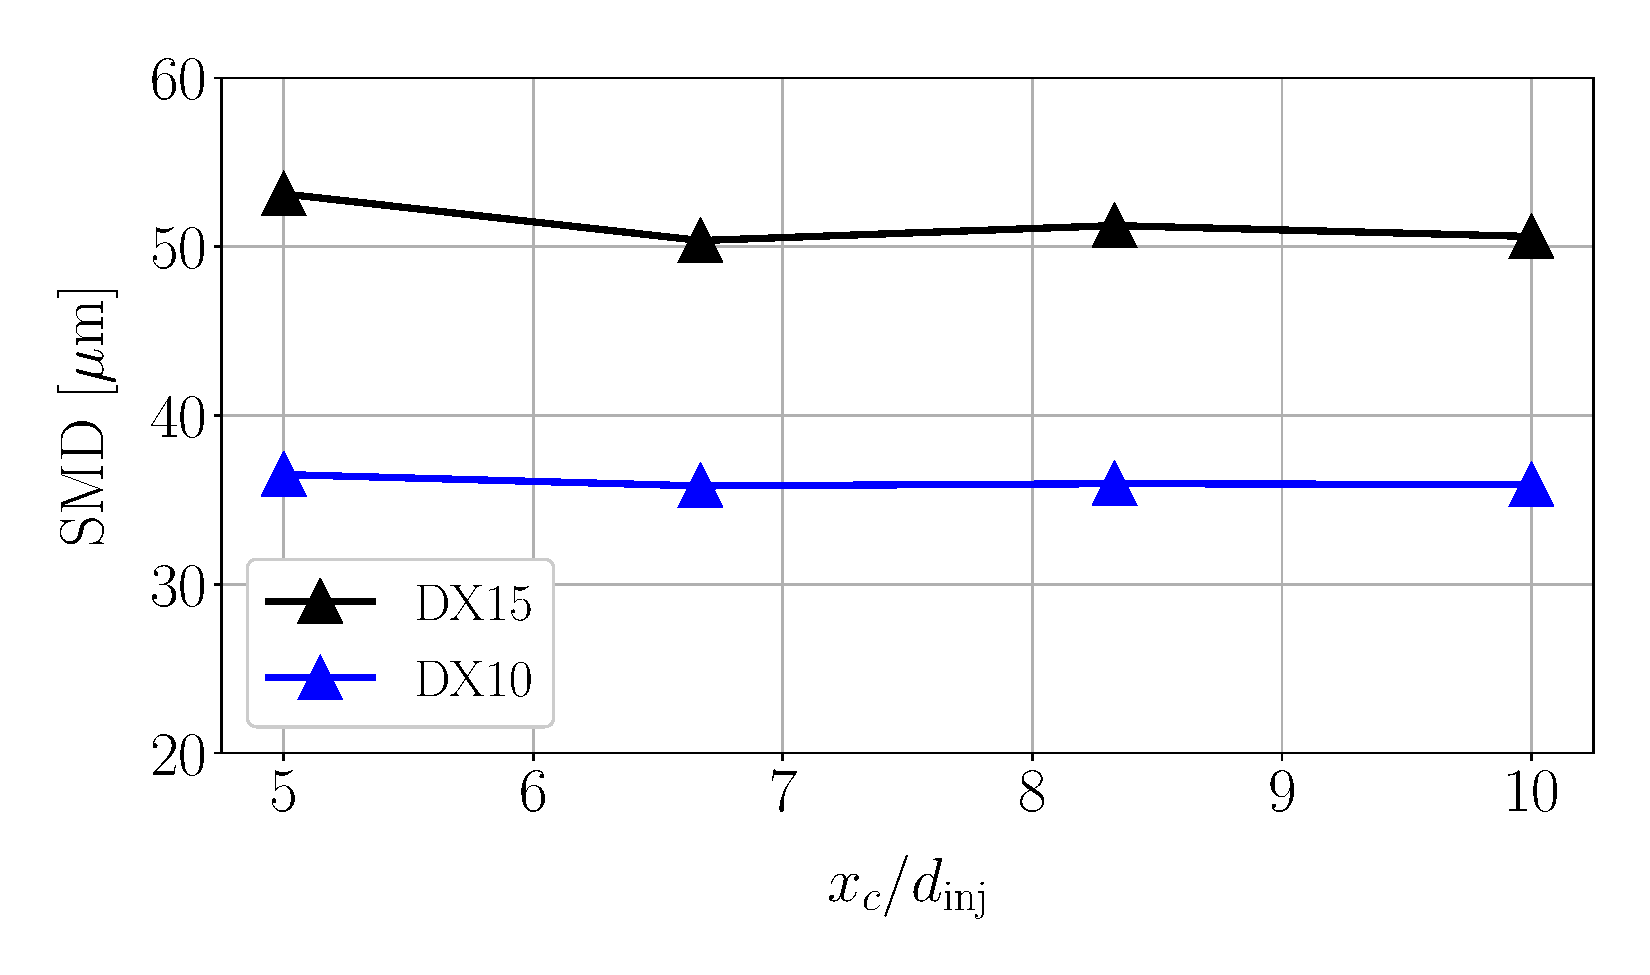
\includegraphics[scale=0.35]{./part3_applications/figures_ch8_resolved/SPRAY_characterization/SMD_values}
   %SMD_values_broken_axis
   \vspace*{-0.2in}
   \caption{Evolution of SMD with axial distance for each simulation.}
   \label{fig:ch8_spray_char_SMD_final}
\end{figure}





\subsection{Liquid velocities}

Mean spray velocities, arithmetic and volume weighted, in axial and vertical directions are shown in Figure \ref{fig:ch8_jicf_liquid_mean_velocities_with_x}. As observed, establishment in axial velocity is reached at $x = 2~\mathrm{mm}$, while the vertical velocities are stable from the first sampling plane. The mean axial velocities do not stabilize at the bulk velocity $u_g = 568~\mathrm{m~s}^{-1}$ since the gaseous field is perturbed due to the presence of the crossflow for the whole range of sampling planes axil locations, as shown in Figure \ref{fig:BIMER_sps_lines_y0_along_x_ux_mean}.   Due to these disturbances, the gaseous field is heterogeneous in space as shown in $\S$\ref{subsec:ch8_turbulent_structures_BIMER} and droplets relax towards values which are different from those found upstream the jet, resulting in mean velocities lower than $u_g$. Regarding mean vertical velocities, these are stabilized in values which are different than $0$, indicating that the spray continues to open vertically with increasing axial distance rather than reach a constant penetration height. This is also attributed to the jet perturbation, since gas streamlines are diverted downstream the jet vertically as displayed in Figure \ref{fig:BIMER_turbulent_structures_plane_y0}. This figure also shows that the vertical component of streamlines for case DX10 is larger than their equivalent in case DX15, which results in larger mean vertical velocities for case DX10 as confirmed by Figure \ref{fig:ch8_jicf_liquid_mean_velocities_with_x}.

\clearpage


%\begin{figure}[ht]
%\centering
%\begin{subfigure}[b]{0.9\textwidth}
%	\centering
%   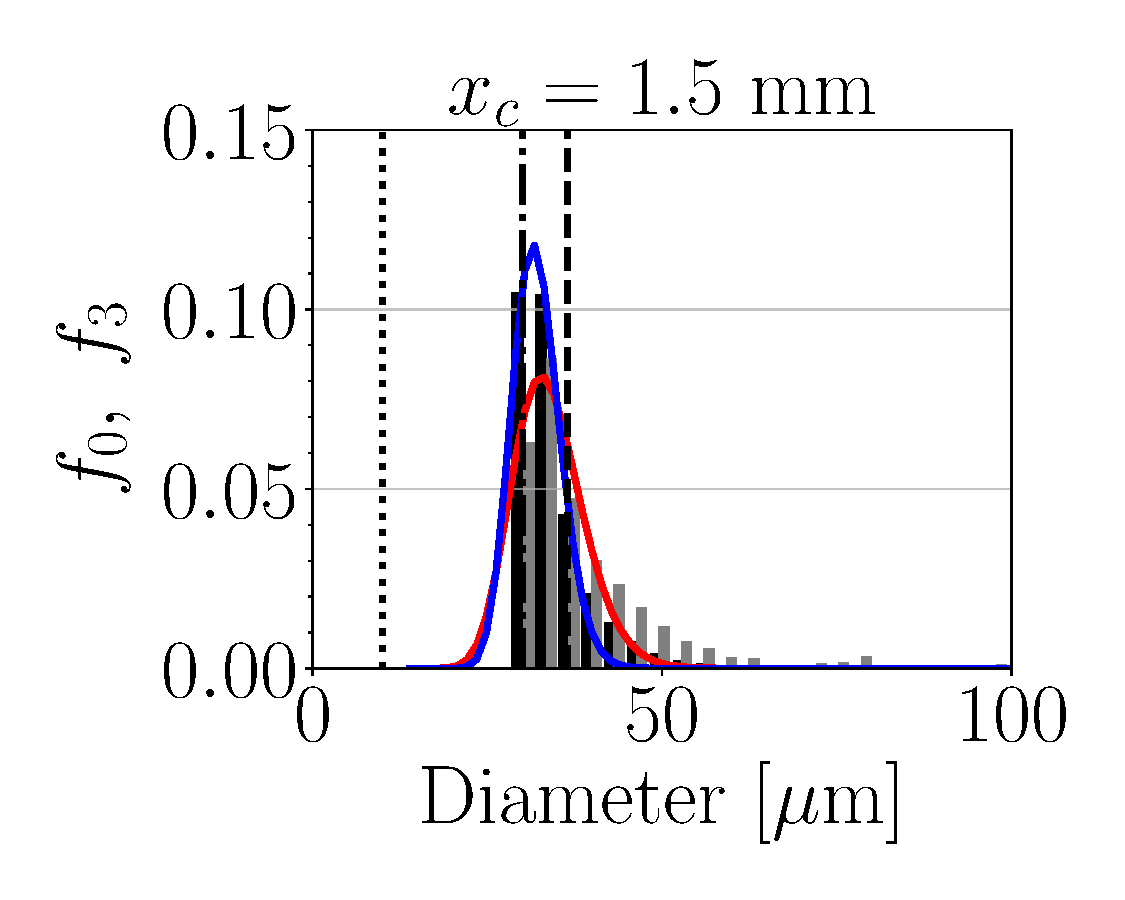
\includegraphics[scale=0.30]{./part3_applications/figures_ch8_resolved/SPRAY_characterization/histograms_size_volume/DX10_xD05p00_histograms}
%   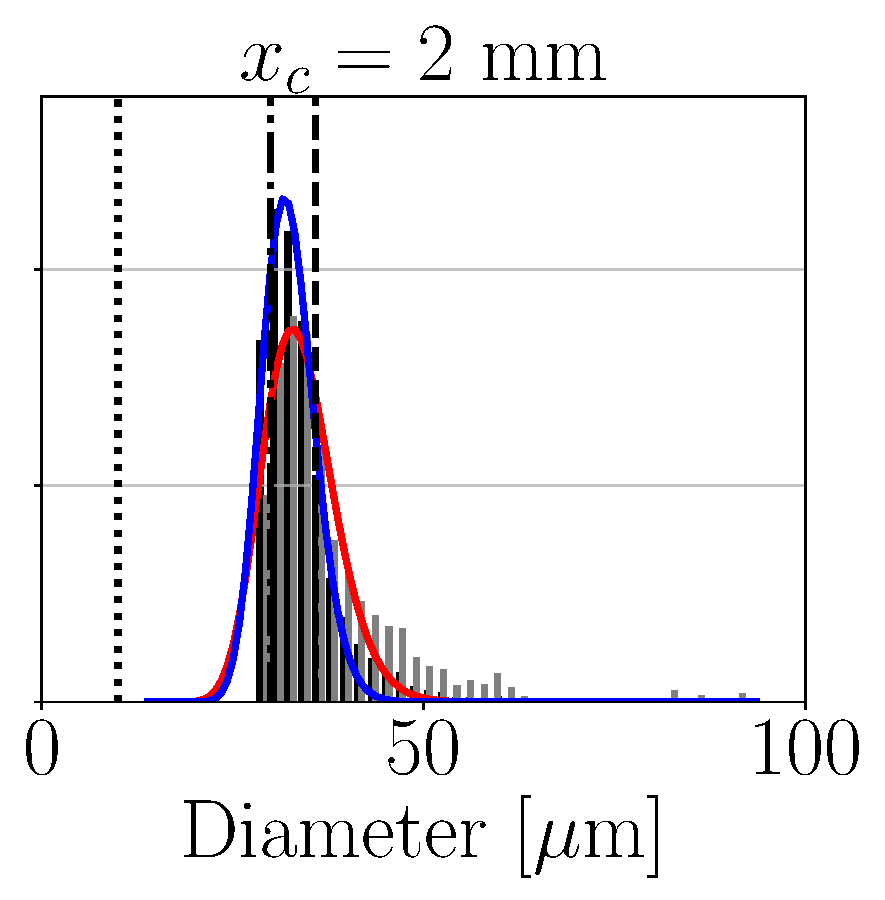
\includegraphics[scale=0.30]{./part3_applications/figures_ch8_resolved/SPRAY_characterization/histograms_size_volume/DX10_xD06p67_histograms}
%	\caption{Case DX10}
%\end{subfigure}
%
%\vskip\baselineskip
%
%\begin{subfigure}[b]{0.9\textwidth}
%	\centering
%   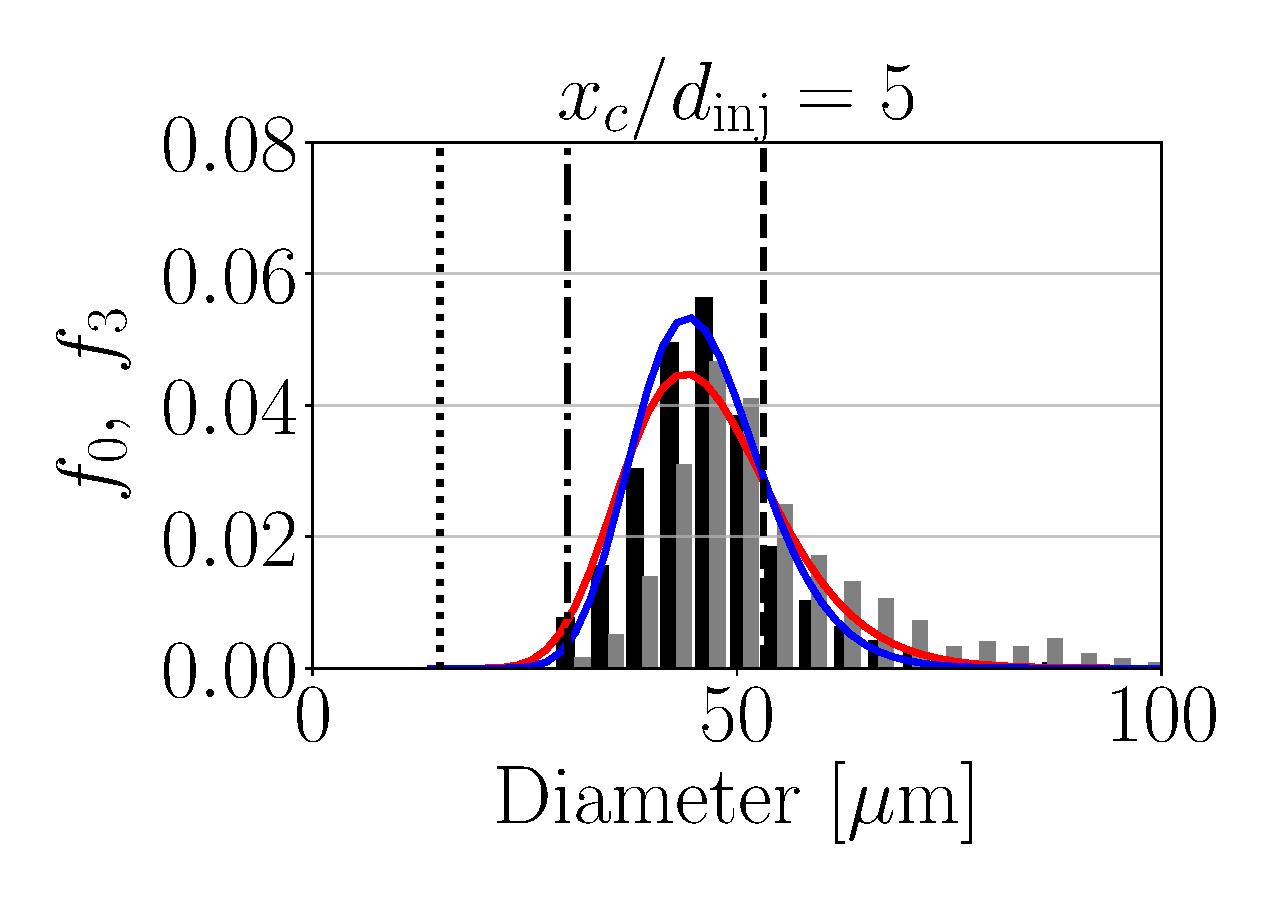
\includegraphics[scale=0.30]{./part3_applications/figures_ch8_resolved/SPRAY_characterization/histograms_size_volume/DX15_xD05p00_histograms}
%   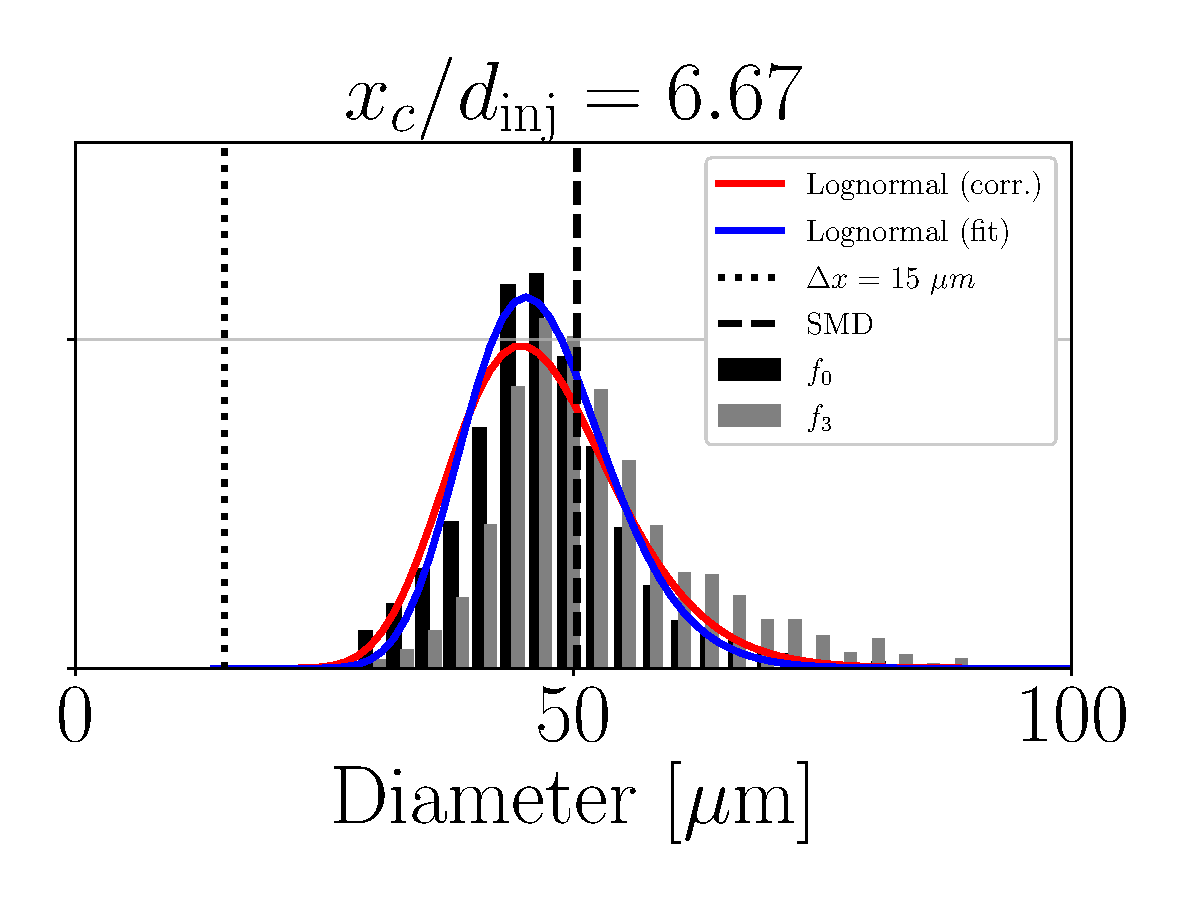
\includegraphics[scale=0.30]{./part3_applications/figures_ch8_resolved/SPRAY_characterization/histograms_size_volume/DX15_xD06p67_histograms}
%	\caption{Case DX15}
%\end{subfigure}
%
%   \caption{Droplets size ($f_0$) and volume ($f_3$) histograms for all BIMER cases}
%\label{fig:ch8_jicf_size_volume_histograms_all}
%\end{figure}


%\begin{figure}[ht]
%\flushleft
%\begin{subfigure}[b]{1.1\textwidth}
%	\flushleft
%   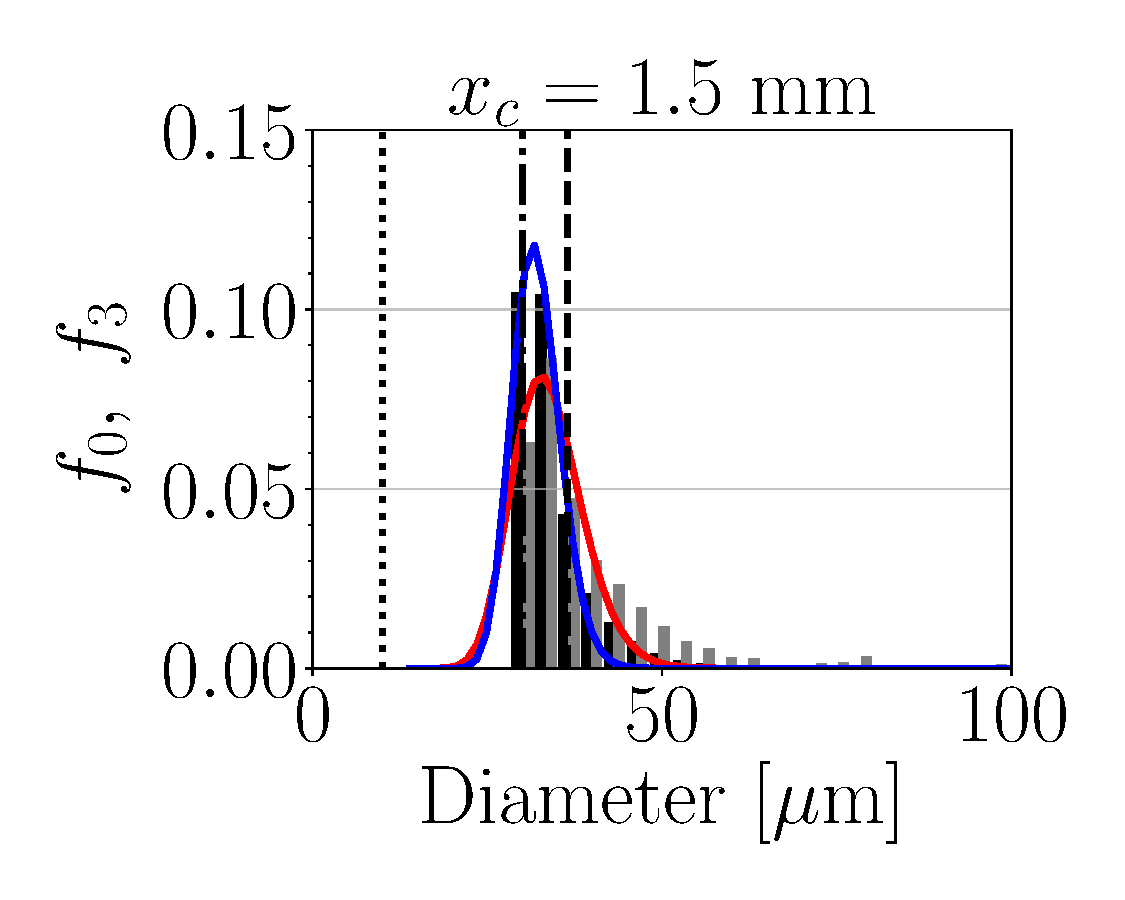
\includegraphics[scale=0.28]{./part3_applications/figures_ch8_resolved/SPRAY_characterization/histograms_size_volume/DX10_xD05p00_histograms}
%   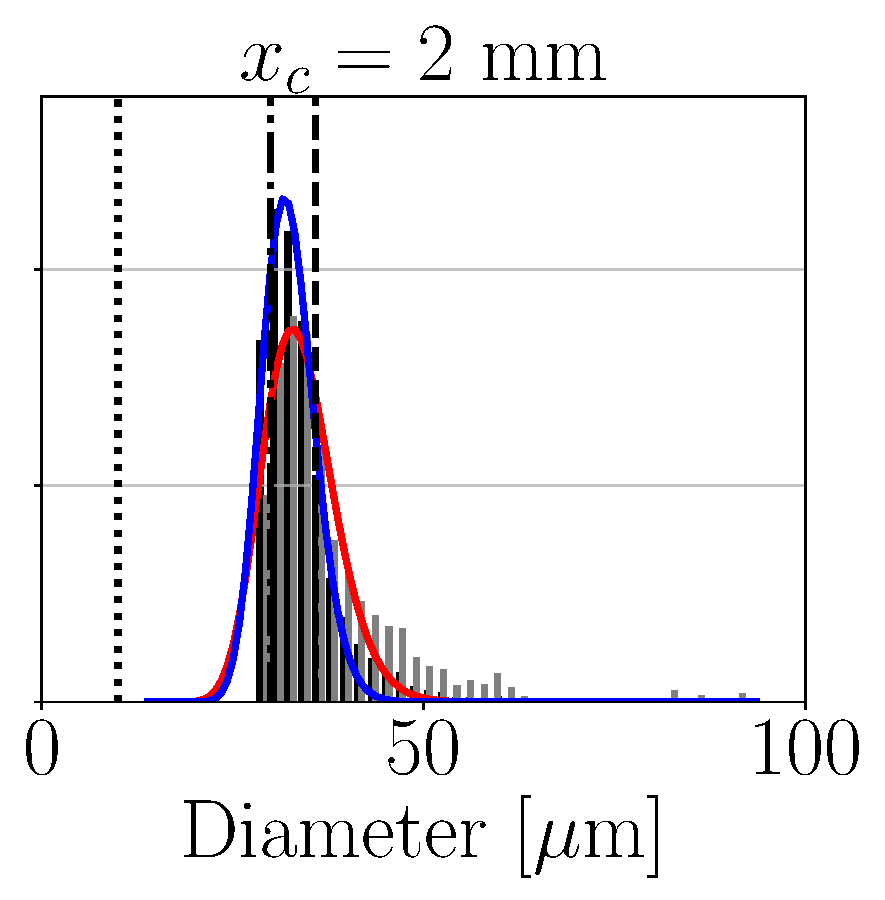
\includegraphics[scale=0.28]{./part3_applications/figures_ch8_resolved/SPRAY_characterization/histograms_size_volume/DX10_xD06p67_histograms}
%   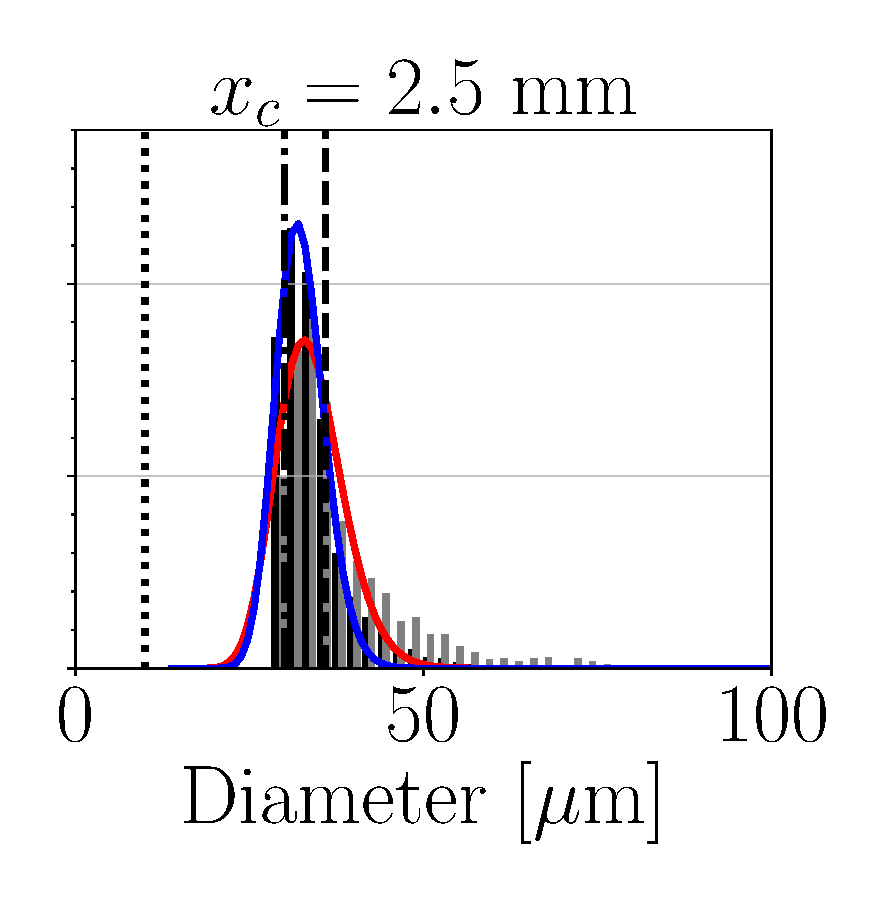
\includegraphics[scale=0.28]{./part3_applications/figures_ch8_resolved/SPRAY_characterization/histograms_size_volume/DX10_xD08p33_histograms}
%	\caption{Case DX10}
%\end{subfigure}
%
%\vskip\baselineskip
%
%\begin{subfigure}[b]{1.1\textwidth}
%	\flushleft
%   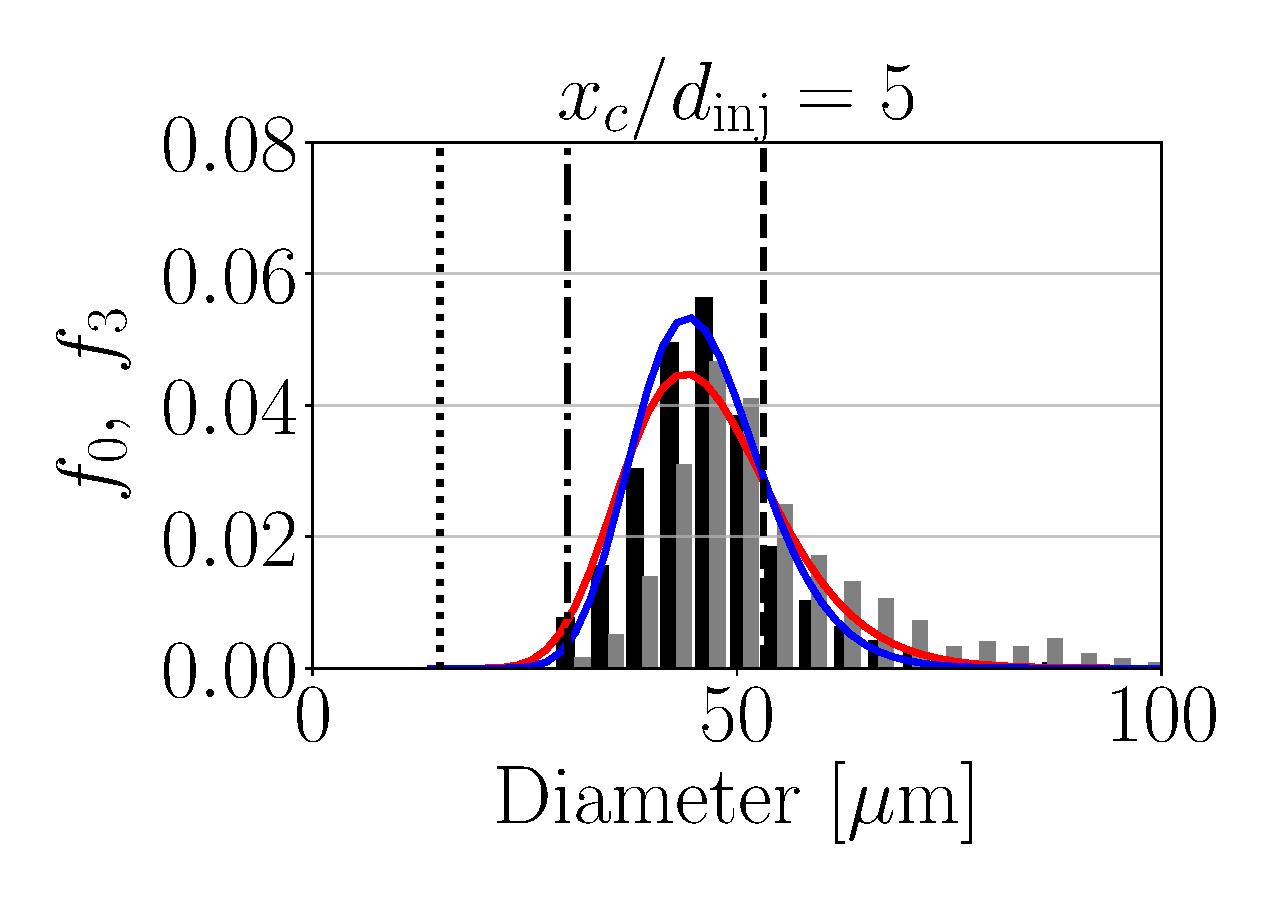
\includegraphics[scale=0.28]{./part3_applications/figures_ch8_resolved/SPRAY_characterization/histograms_size_volume/DX15_xD05p00_histograms}
%   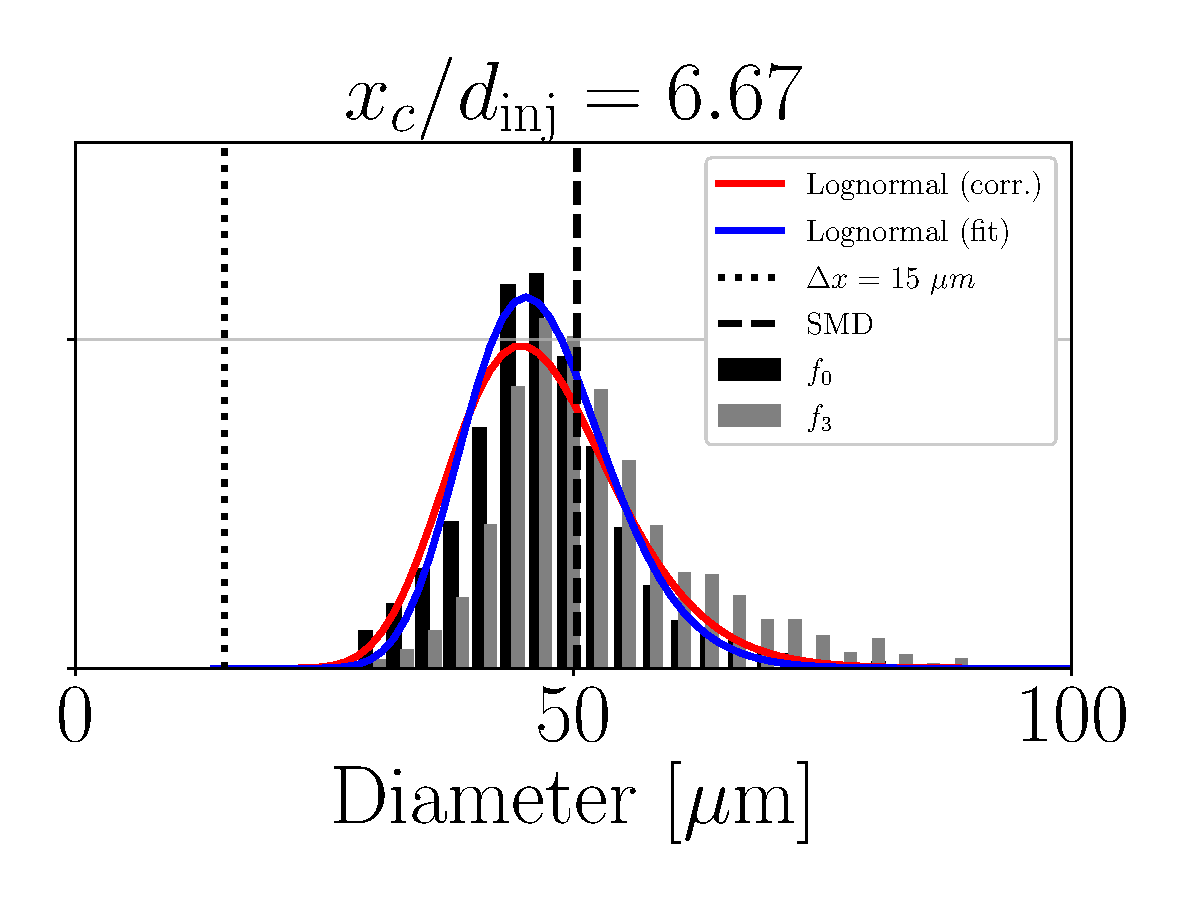
\includegraphics[scale=0.28]{./part3_applications/figures_ch8_resolved/SPRAY_characterization/histograms_size_volume/DX15_xD06p67_histograms}
%   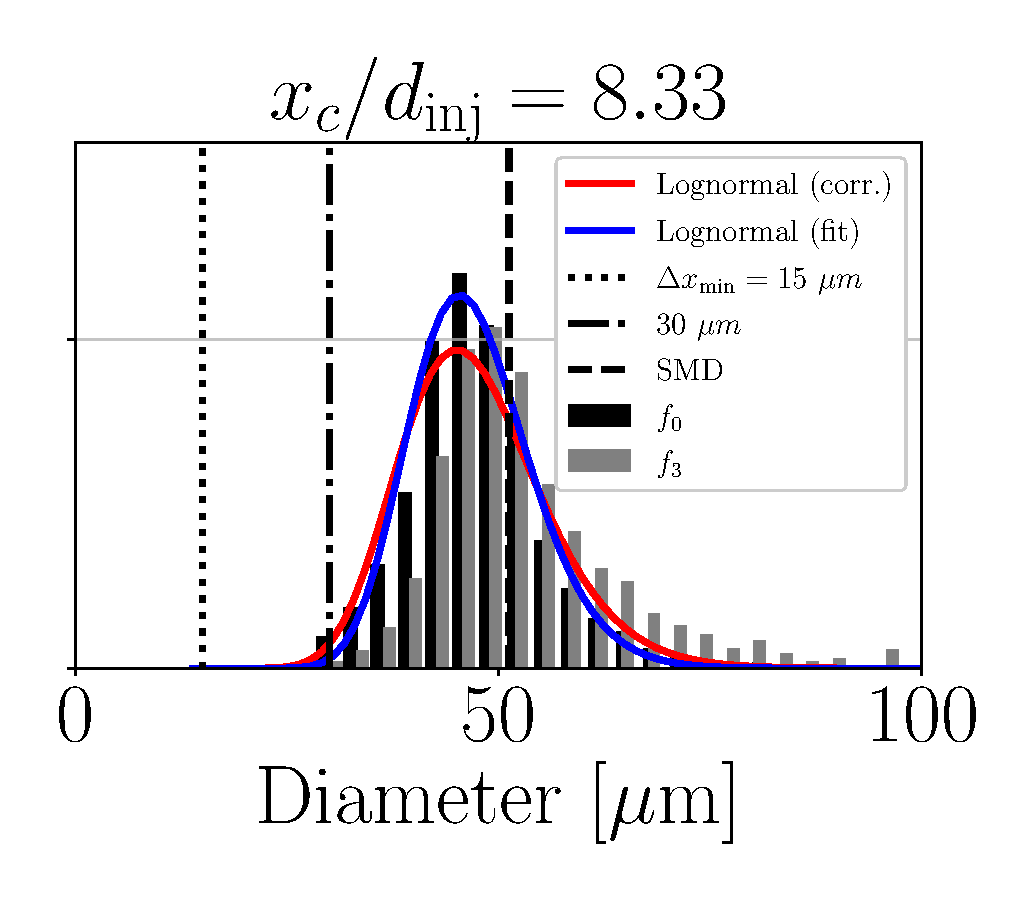
\includegraphics[scale=0.28]{./part3_applications/figures_ch8_resolved/SPRAY_characterization/histograms_size_volume/DX15_xD08p33_histograms}
%	\caption{Case DX15}
%\end{subfigure}
%
%   \caption{Droplets size ($f_0$) and volume ($f_3$) histograms for all BIMER cases}
%\label{fig:ch8_jicf_size_volume_histograms_all}
%\end{figure}

\begin{figure}[ht]
\flushleft
%\begin{subfigure}[b]{1.1\textwidth}
%	\flushleft
%   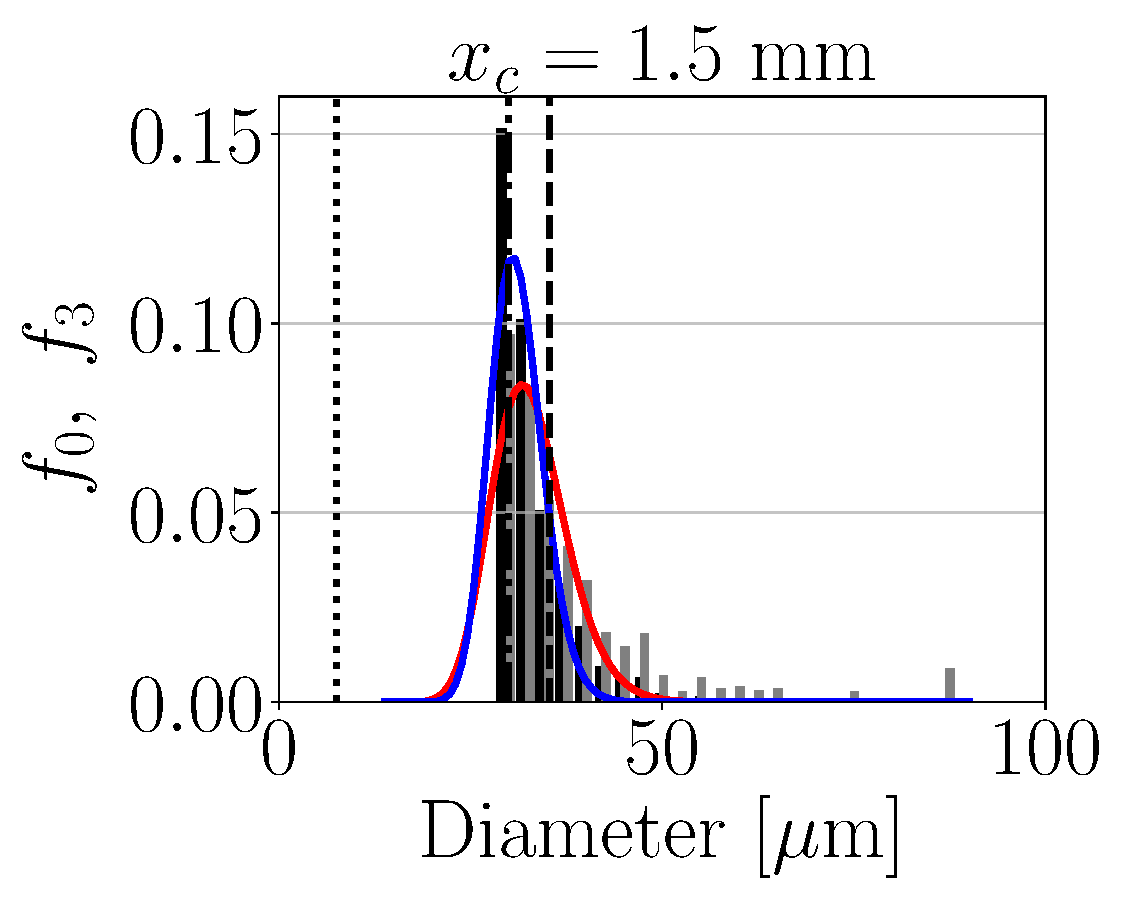
\includegraphics[scale=0.28]{./part3_applications/figures_ch8_resolved/SPRAY_characterization/histograms_size_volume/DX07_xD05p00_histograms}
%   \hspace*{-0.15in}
%   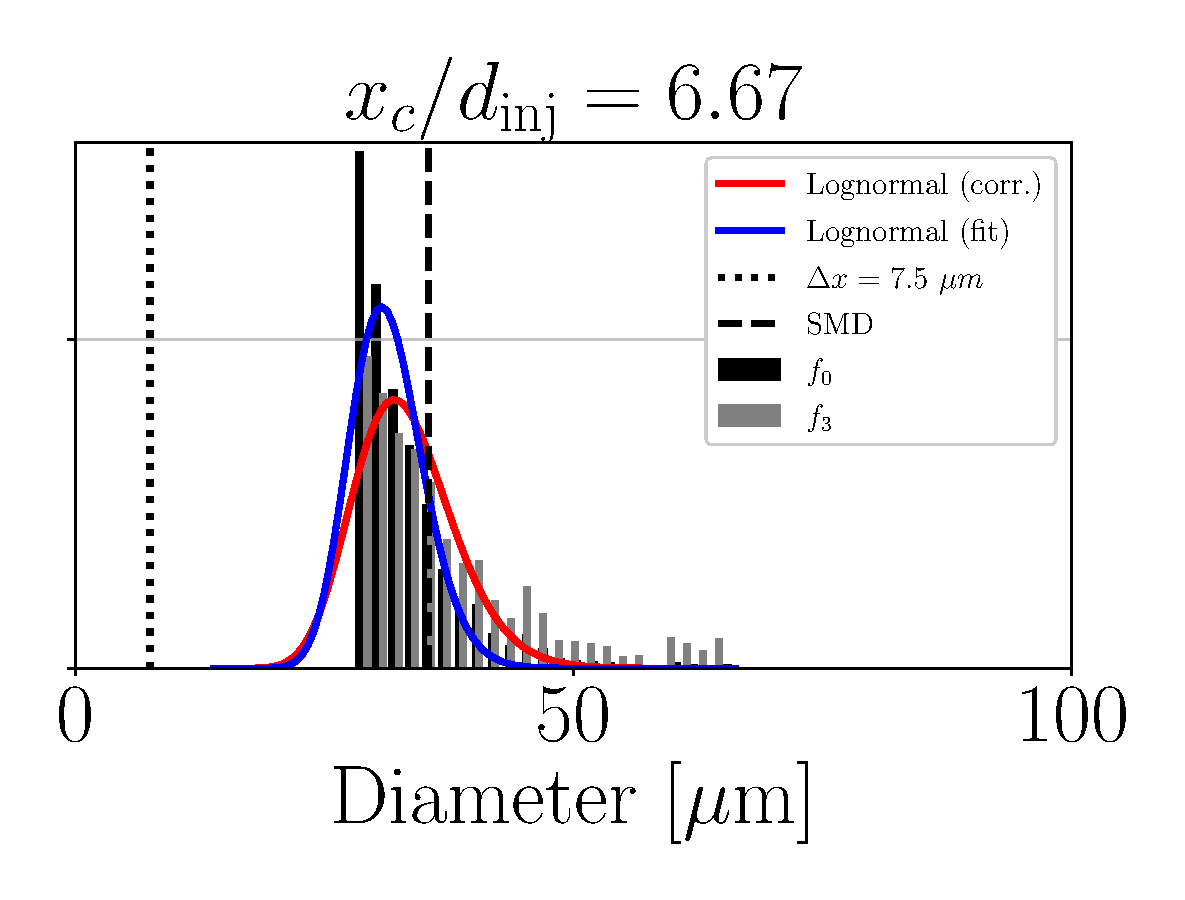
\includegraphics[scale=0.28]{./part3_applications/figures_ch8_resolved/SPRAY_characterization/histograms_size_volume/DX07_xD06p67_histograms}
%   \hspace*{-0.15in}
%   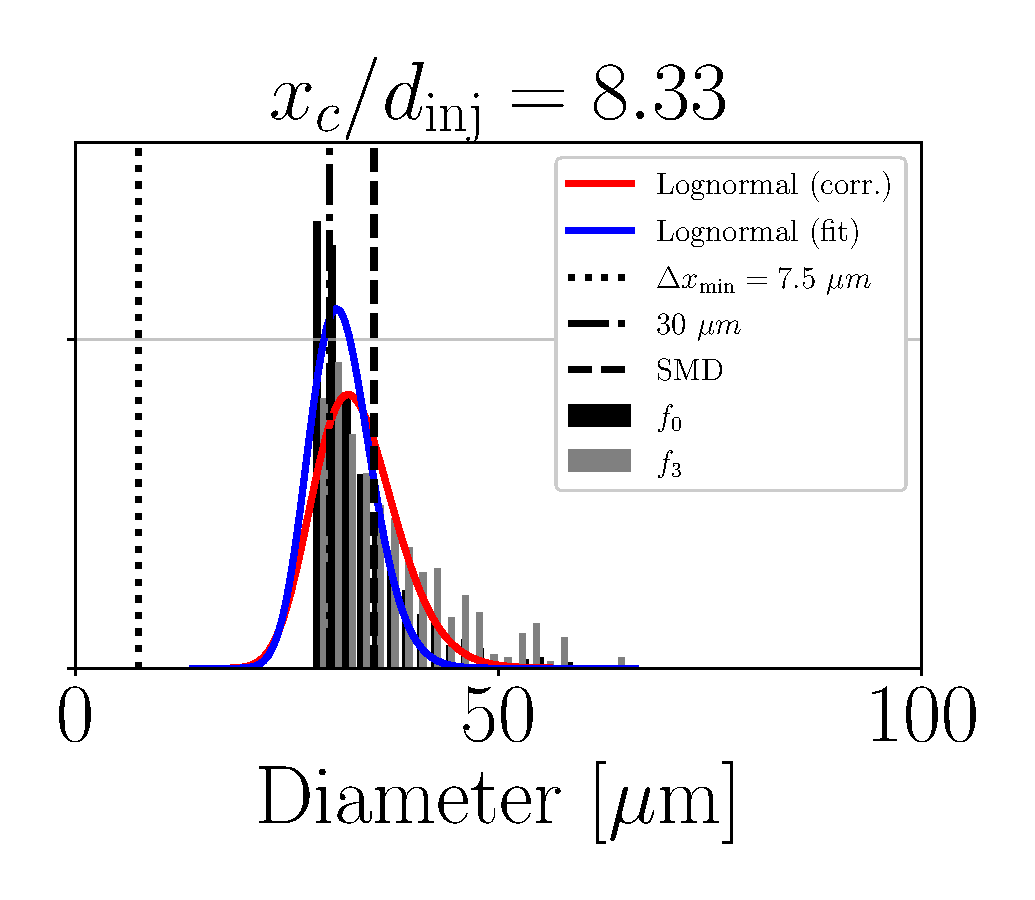
\includegraphics[scale=0.28]{./part3_applications/figures_ch8_resolved/SPRAY_characterization/histograms_size_volume/DX07_xD08p33_histograms}
%   \hspace*{-0.15in}
%   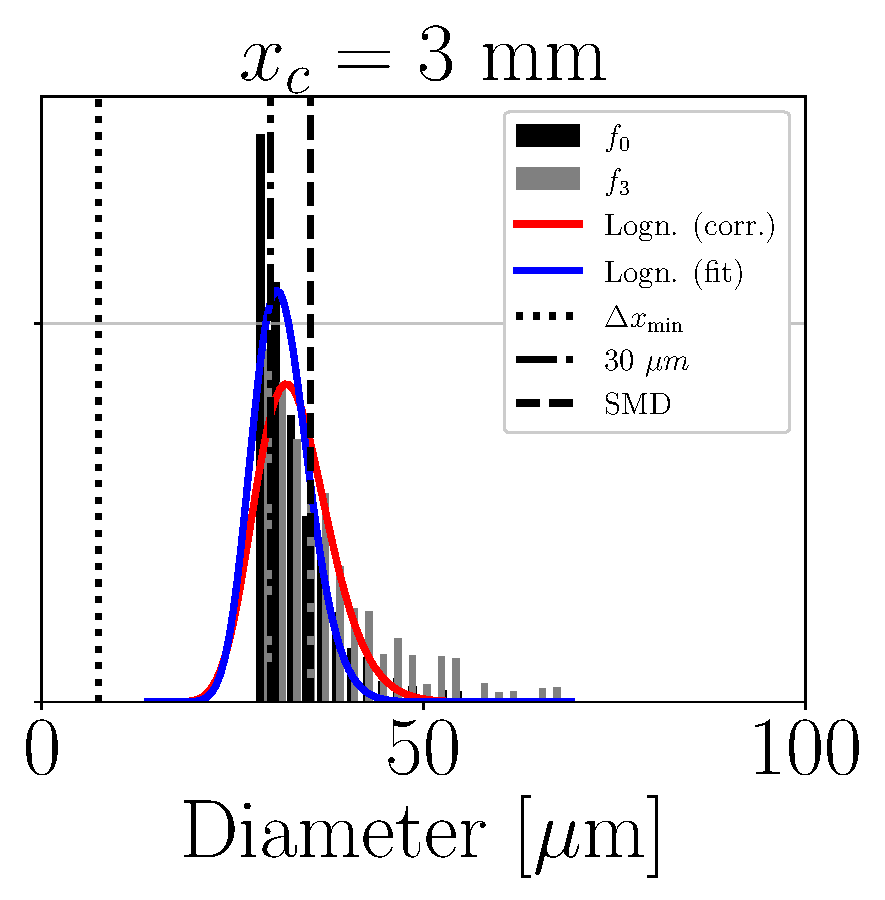
\includegraphics[scale=0.28]{./part3_applications/figures_ch8_resolved/SPRAY_characterization/histograms_size_volume/DX07_xD10p00_histograms}
%	\caption{Case DX07}
%\end{subfigure}
%
%\vskip\baselineskip
\begin{subfigure}[b]{1.1\textwidth}
	\flushleft
   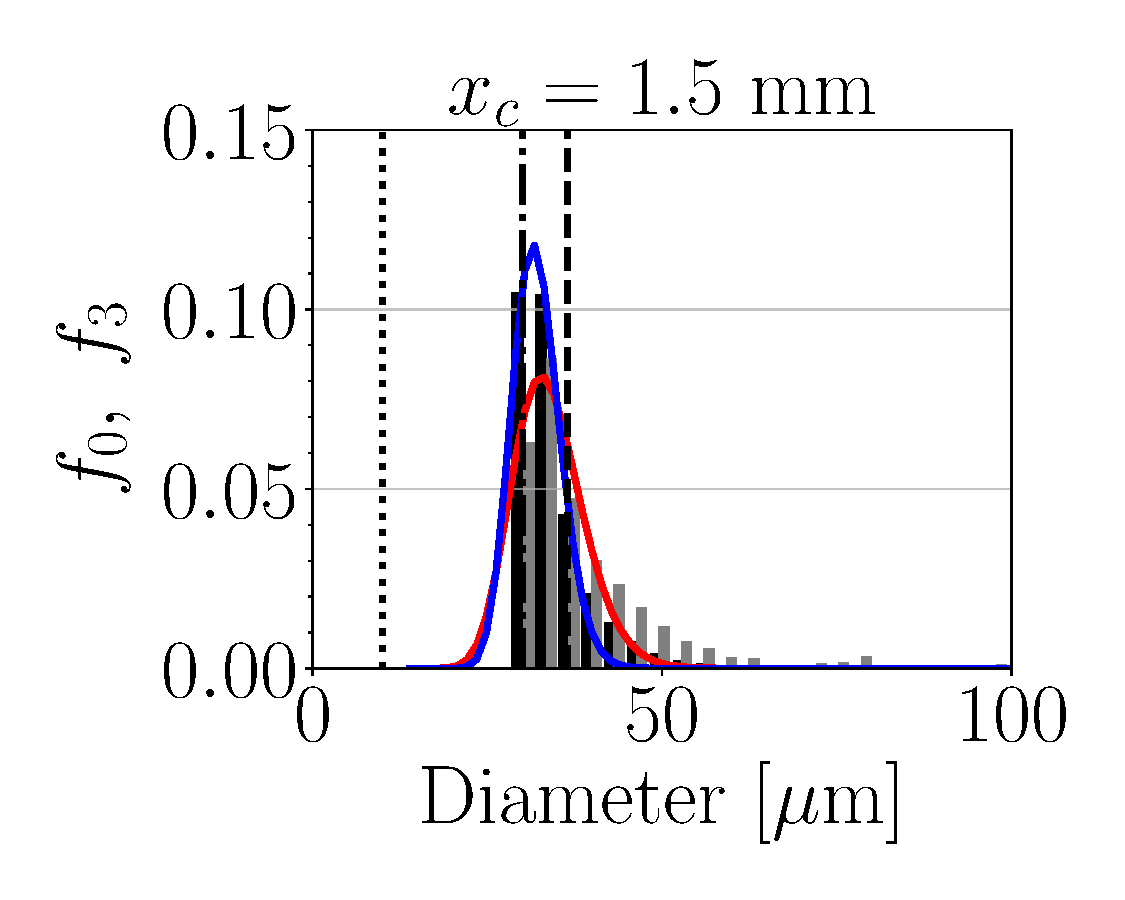
\includegraphics[scale=0.28]{./part3_applications/figures_ch8_resolved/SPRAY_characterization/histograms_size_volume/DX10_xD05p00_histograms}
   \hspace*{-0.15in}
   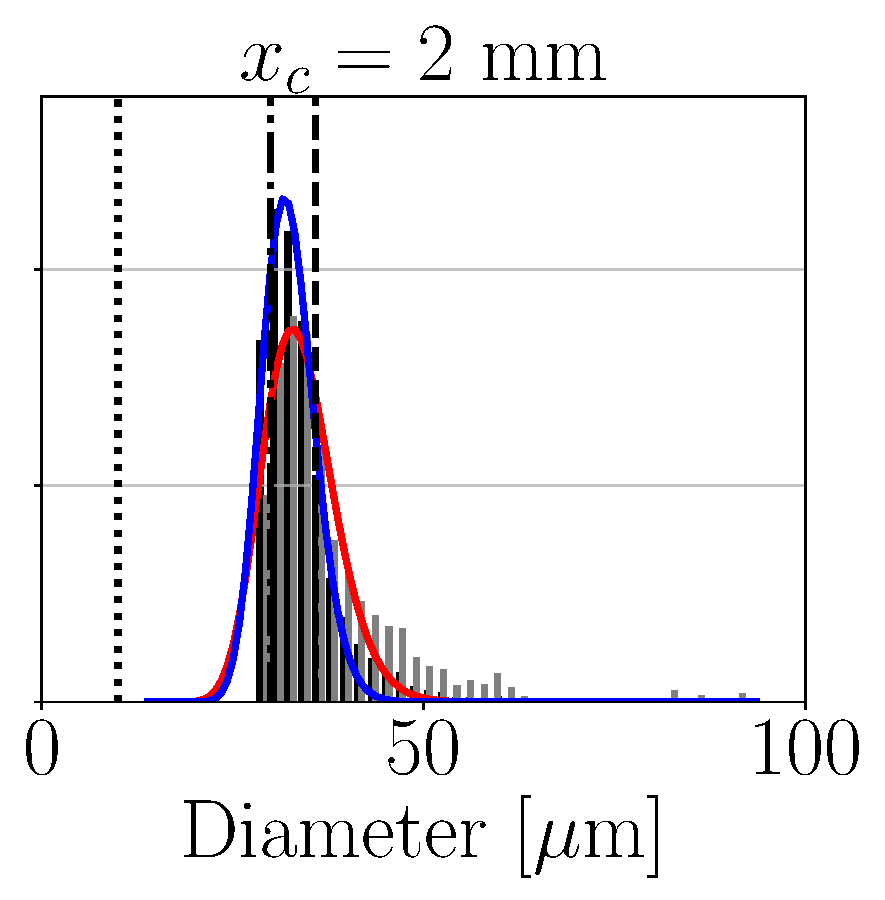
\includegraphics[scale=0.28]{./part3_applications/figures_ch8_resolved/SPRAY_characterization/histograms_size_volume/DX10_xD06p67_histograms}
   \hspace*{-0.15in}
   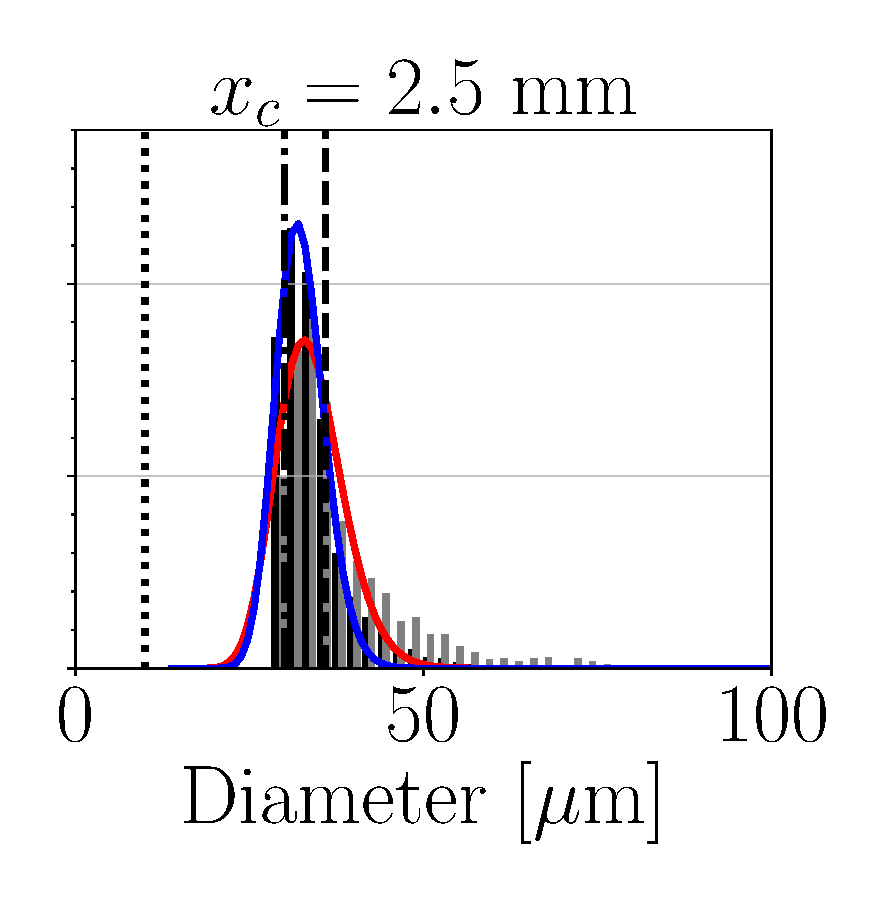
\includegraphics[scale=0.28]{./part3_applications/figures_ch8_resolved/SPRAY_characterization/histograms_size_volume/DX10_xD08p33_histograms}
   \hspace*{-0.15in}
   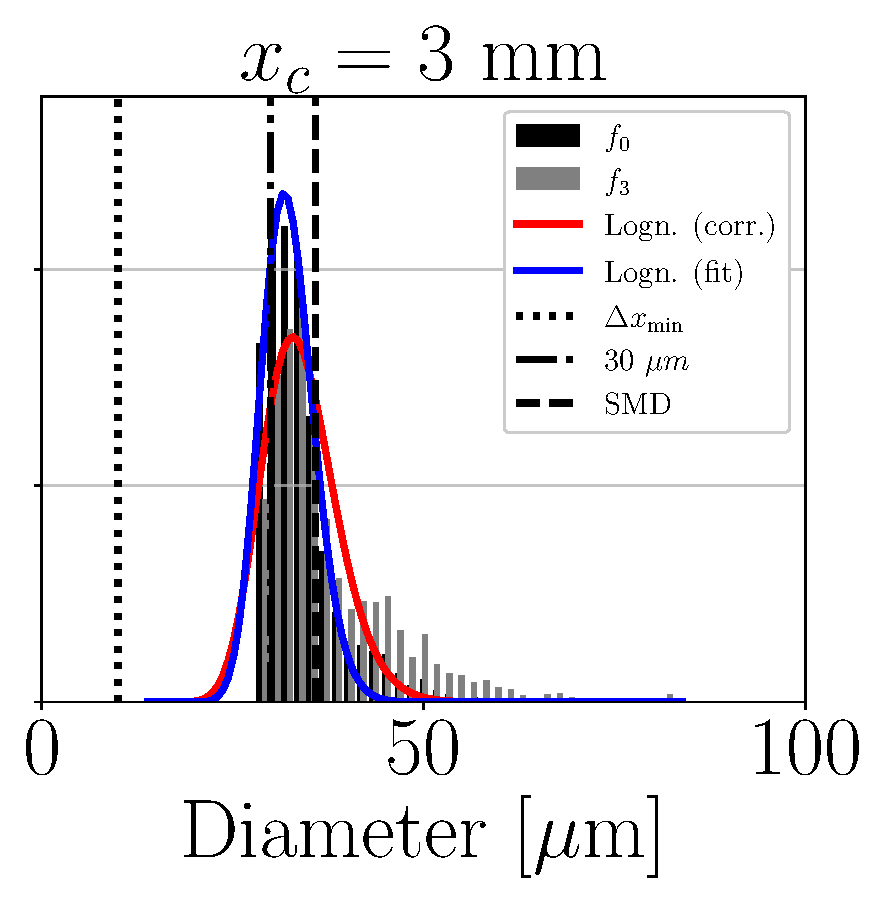
\includegraphics[scale=0.28]{./part3_applications/figures_ch8_resolved/SPRAY_characterization/histograms_size_volume/DX10_xD10p00_histograms}
	\caption{Case DX10}
\end{subfigure}

\vskip\baselineskip

\begin{subfigure}[b]{1.1\textwidth}
	\flushleft
   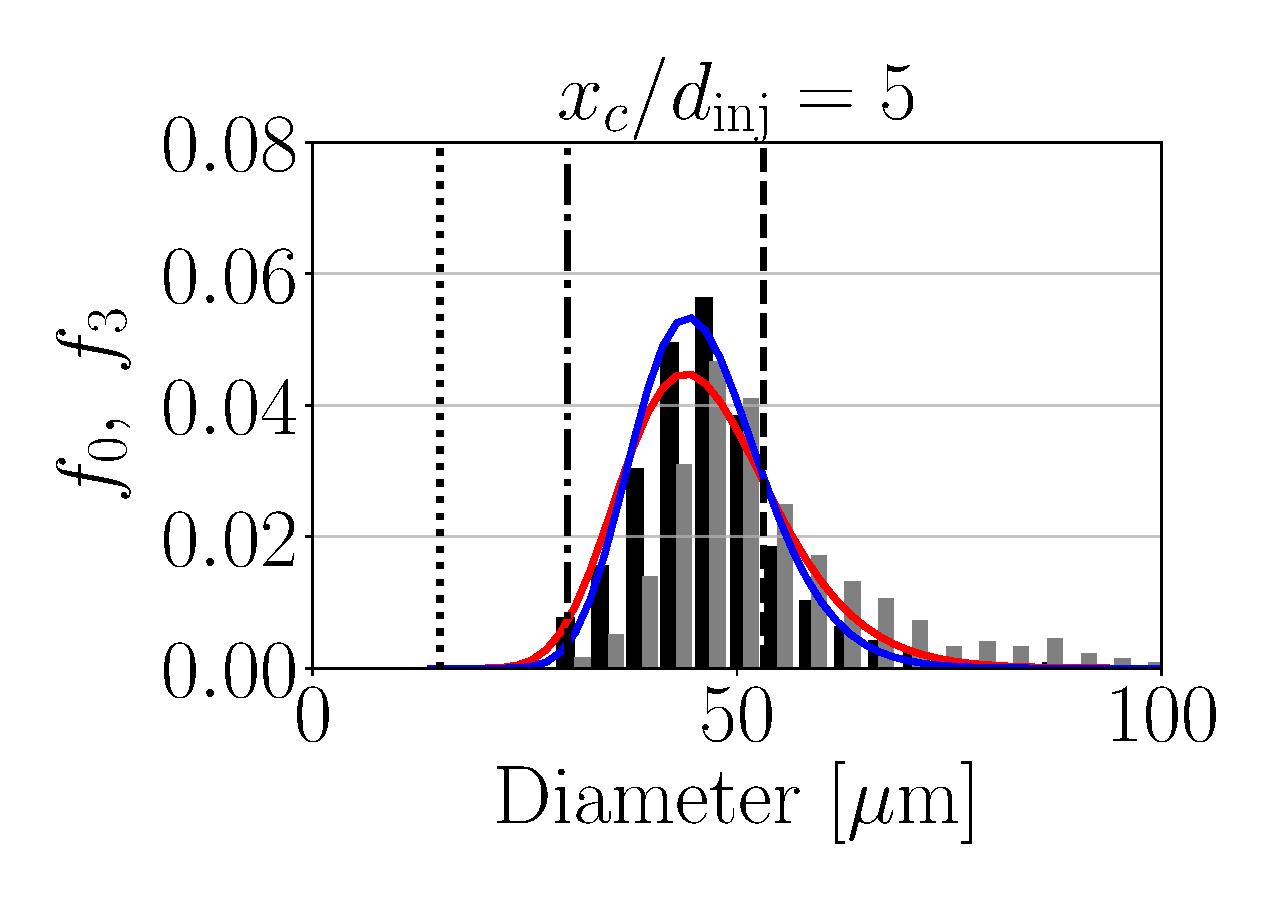
\includegraphics[scale=0.28]{./part3_applications/figures_ch8_resolved/SPRAY_characterization/histograms_size_volume/DX15_xD05p00_histograms}
   \hspace*{-0.15in}
   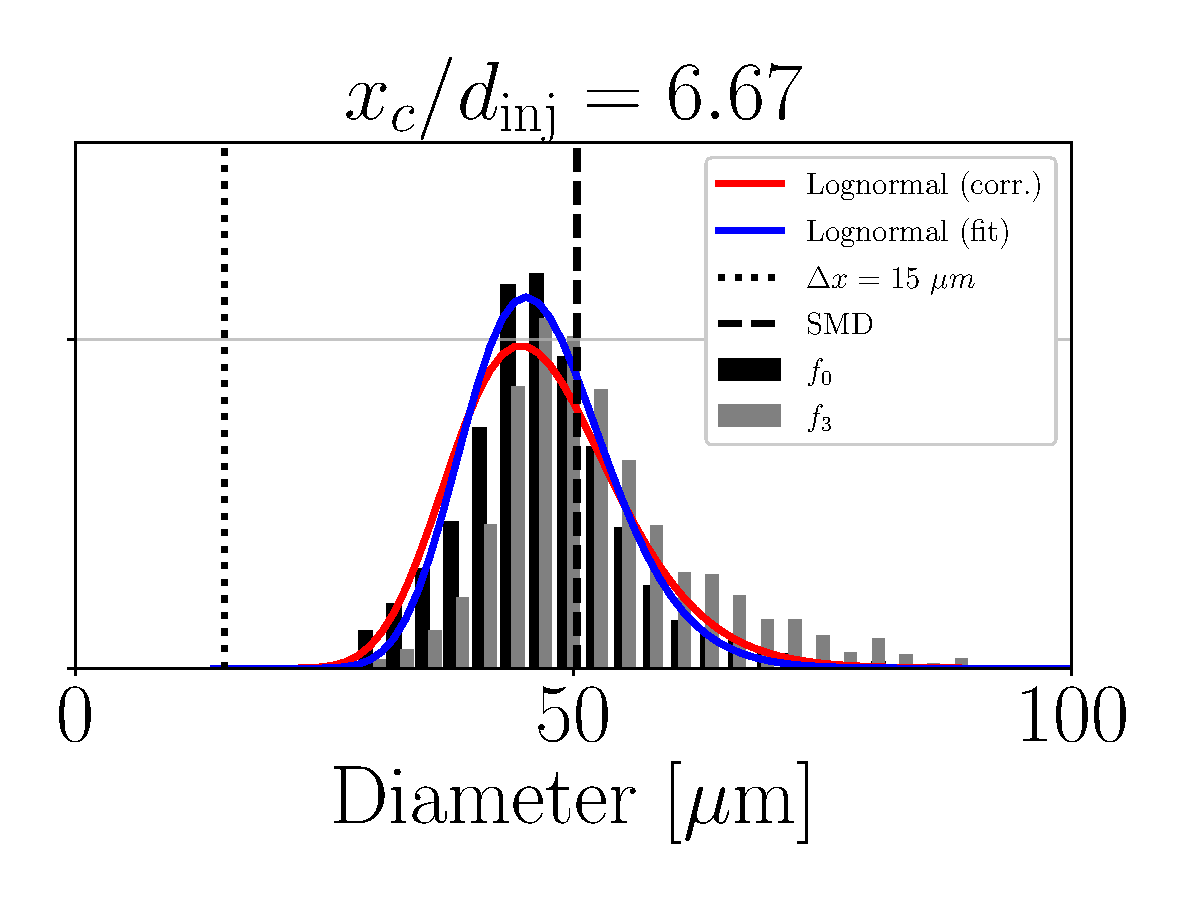
\includegraphics[scale=0.28]{./part3_applications/figures_ch8_resolved/SPRAY_characterization/histograms_size_volume/DX15_xD06p67_histograms}
   \hspace*{-0.15in}
   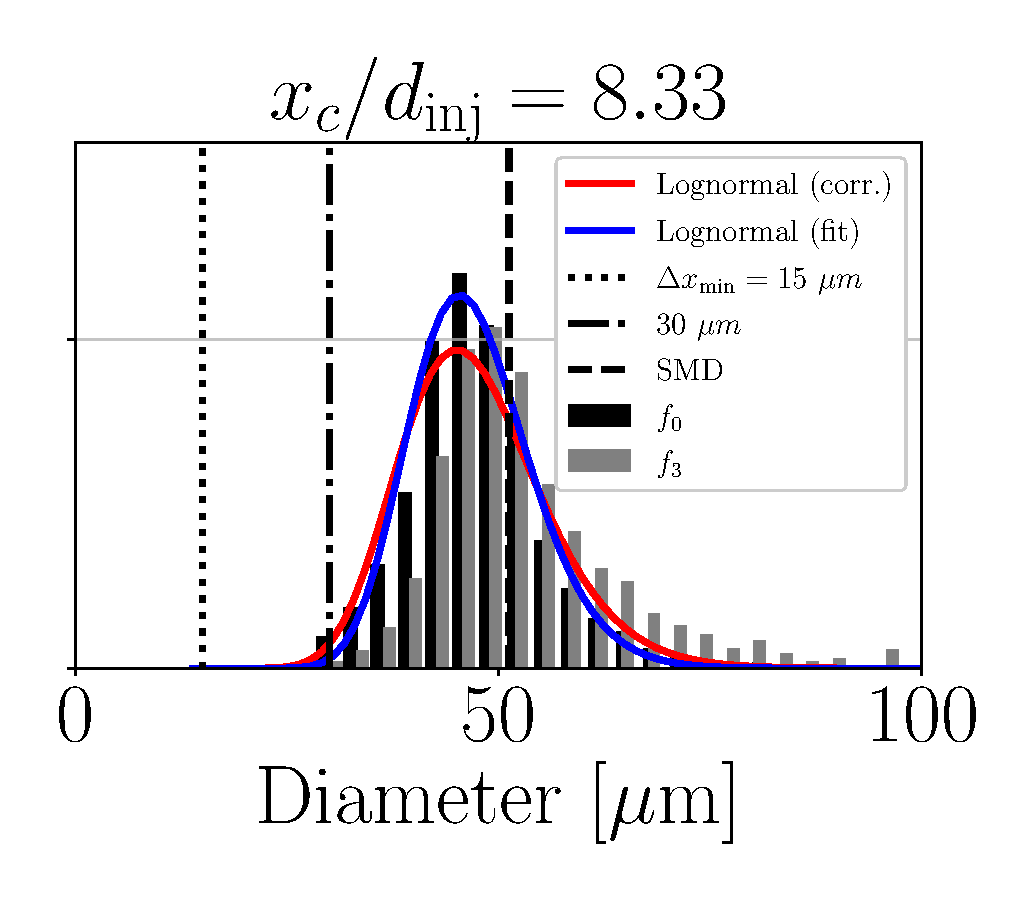
\includegraphics[scale=0.28]{./part3_applications/figures_ch8_resolved/SPRAY_characterization/histograms_size_volume/DX15_xD08p33_histograms}
   \hspace*{-0.15in}
   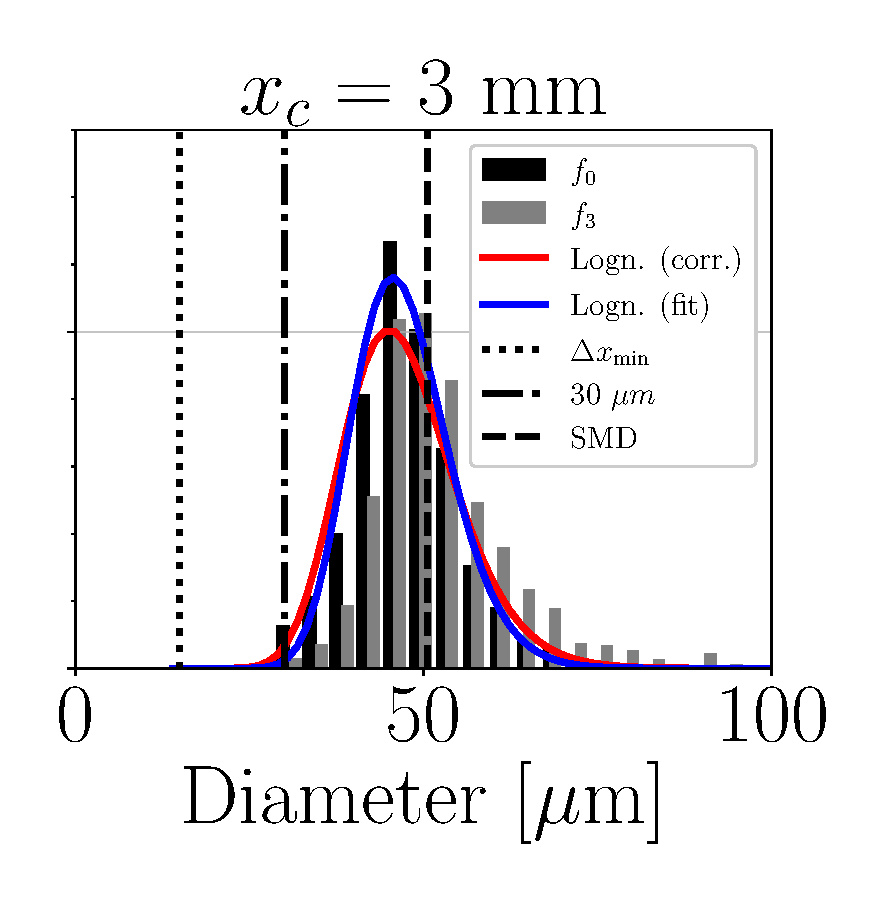
\includegraphics[scale=0.28]{./part3_applications/figures_ch8_resolved/SPRAY_characterization/histograms_size_volume/DX15_xD10p00_histograms}
	\caption{Case DX15}
\end{subfigure}

   \caption{Droplets size ($f_0$) and volume ($f_3$) histograms for all BIMER cases}
\label{fig:ch8_jicf_size_volume_histograms_all}
\end{figure}

\begin{figure}[ht]
\flushleft
\begin{subfigure}[b]{1.0\textwidth}
	\flushleft
   \includegraphics[scale=0.25]{./part3_applications/figures_ch8_resolved/SPRAY_characterization/velocities/ux_mean}
   %\hspace*{0.2in}
   %\includegraphics[scale=0.25]{./part3_applications/figures_ch8_resolved/SPRAY_characterization/velocities/uy_mean}
   \hspace*{0.2in}
   %\hfill
   \includegraphics[scale=0.25]{./part3_applications/figures_ch8_resolved/SPRAY_characterization/velocities/uz_mean}
\end{subfigure}

   \caption[Sampled mean liquid velocities for all cases]{Mean velocities in axial, lateral and vertical crossflow directions. Solid lines indicate arithmetic average velocities, while dashed ones indicate volume-weighted average velocities.}
\label{fig:ch8_jicf_liquid_mean_velocities_with_x}
\end{figure}


\vspace*{-0.20in}


\subsection{Deformation of liquid structures}
\label{subsec:ch8_def_liquid_structures}

Figure \ref{fig:ch8_jicf_liquid_mean_deformation_with_x_condensed} shows evolution of volume-weighted averages of deformation parameters for all cases. Stablishment with axial distance is obtained at $x_c = 2$ mm, as for the other previous magnitudes discussed. Considering the sphericity criteria to be for droplets presenting $\beta > 0.5, \alpha < 2$, it is seen that mean values are stablished outside the sphericity range. A view at the $\alpha-\beta$ scatterplots in Figure \ref{fig:ch8_jicf_global_scatterplots_deformation} shows that most droplets are located outside this sphericity region (enclosed by the thick black lines): the percentages of spherical droplets is 5 and 13 $\%$ for DX15 and DX10 respectively at plane $x = 2$ mm . Such percentage does not vary considerable further downstream, indicating that transported droplets are mostly deformed. 

\clearpage

\begin{figure}[ht]
\centering
   \includegraphics[scale=0.25]{./part3_applications/figures_ch8_resolved/SPRAY_characterization/deformation/deformation_both_alpha_beta_mean}
   \caption{Mean deformation parameters for BIMER simulations}
\label{fig:ch8_jicf_liquid_mean_deformation_with_x_condensed}
\end{figure}


\begin{figure}[ht]
\centering
\begin{subfigure}[b]{0.4\textwidth}
	\centering
	\hspace*{-0.2in}
   \includegraphics[scale=0.3]{./part3_applications/figures_ch8_resolved/SPRAY_characterization/deformation/scatter_alpha_beta_DX10.png}
\end{subfigure}
\begin{subfigure}[b]{0.4\textwidth}
	\centering
	\hspace*{0.35in}
   \includegraphics[scale=0.3]{./part3_applications/figures_ch8_resolved/SPRAY_characterization/deformation/scatter_alpha_beta_DX15.png}
\end{subfigure}
\begin{subfigure}[b]{0.1\textwidth}
	\centering
	\hspace*{0.35in}
   \includegraphics[scale=0.5]{./part3_applications/figures_ch8_resolved/SPRAY_characterization/deformation/scatterplots_colorbar_D_with_blank_space.png}
\end{subfigure}
   \caption[Scatterplots of deformation parameters $\alpha$ - $\beta$ for cases DX10, DX15 at plane $x_c = 2$ mm ]{Scatterplots of deformation parameters $\alpha$ - $\beta$ for cases DX10, DX15 at plane $x_c = 2$ mm. Droplets are coloured and scaled by their equivalent diameter. Thick, black lines enclose the region where droplets are spherical according to the criteria defined in the text}
\label{fig:ch8_jicf_global_scatterplots_deformation}
\end{figure}




\section{Smart Lagrangian Injectors}
\label{sec:ch8_learning_SLI_in_BIMER}






\newcommand\scaleSLIBIMER{0.175}

SLIs are obtained by applying the discretization process described in $\S$\ref{subsec:SLI_spatial_discretization} to the previously shown sprays. Since it was shown in the former section that convergence was achieved for most magnitudes at $x_c = 2$ mm, SLIs are shown here only for the sampling planes at $x_c = 1.5, 2$ mm. Results are shown in Figures \ref{fig:injectors_sli_BIMER_DX10_xD05} to  \ref{fig:injectors_sli_BIMER_DX15_xD06p67}. The SMDs maps show a circular structure in which large values are obtained at the center of the spray and diameters are reduced further away. Fluxes maps exhibit a circular structure which is typical from all liquids JICF. These maps show maximum flux values located at around $y_c = 0$ and symmetry with respect to this axis for case DX10, which indicates that the crossflow direction has been properly chosen. Axial velocity maps show a classical low-velocity region in the bottom part, central region of the spray which corresponds to the disturbance effect of the spray, while the vertical velocity maps display the classical layered structure with increasing velocity along the vertical direction $z_c$, hence indicating that the spray continues to penetrate further away as it is convected downstream. Large differences with respect to the classical JICF of Chapter \ref{ch5:jicf_resolved_simulations} are observed for the lateral velocity $v_c$, since in this case the profiles are not symmetric with respect to the $y_c = 0$ axis due to the swirl component of the air. With respect to the convergence maps, it is shown that more converged probes are obtained for the fine resolution than for the coarse one even though the total physical time simulated is lower. The same observation was done for the classical JICF as detailed in $\S$\ref{subsec:ch5_learning_SLI}: it can be concluded then that a finer mesh makes SLI converge with lower physical time simulated. It is worth noting that convergence has only been defined according to the droplet size distribution as indicated by Eq. (\ref{eq:MSE_definition}): further research includes testing other $MSE$ functions accounting for other magnitudes such as velocities. Nevertheless, the $SMD$ and velocity maps obtained for the coarse resolution (Figures \ref{fig:injectors_sli_BIMER_DX15_xD05} and \ref{fig:injectors_sli_BIMER_DX15_xD06p67}) seem \textsl{less converged} than their equivalents for the fine case (Figures \ref{fig:injectors_sli_BIMER_DX10_xD05} and \ref{fig:injectors_sli_BIMER_DX10_xD06p67}) due to the less smooth contours obtained. This might indicate that the resolution DX15 is too coarse to simulate BIMER, and therefore only the SLI obtained for case DX10 will be used to perform the dispersed phase simulations from Chapter \ref{ch9:BIMER_lagrangian}.


\subsubsection*{Case DX10}



%%%%%%%%%%%%%%%% DX10, xD = 5


\begin{figure}[h!]
\centering
\begin{subfigure}[b]{0.3\textwidth}
	\centering
   \includegraphics[scale=\scaleSLIBIMER]{./part3_applications/figures_ch8_resolved/injectors_SLI/dx10_xD05p00_SMD_map}
   %\caption{Case UG100\_DX20: crossflow planes}
   %\label{} 
\end{subfigure}
   \hspace{0.17in}
\begin{subfigure}[b]{0.3\textwidth}
	\centering
   \includegraphics[scale=\scaleSLIBIMER]{./part3_applications/figures_ch8_resolved/injectors_SLI/dx10_xD05p00_volume_flux_map}
   %\caption{Case UG100\_DX20: filming planes}
   %\label{}
\end{subfigure}
   \hspace{0.17in}
\begin{subfigure}[b]{0.3\textwidth}
	\centering
   \includegraphics[scale=\scaleSLIBIMER]{./part3_applications/figures_ch8_resolved/injectors_SLI/dx10_xD05p00_convergence_map}
   %\caption{Case UG100\_DX10: crossflow planes}
   %\label{} 
\end{subfigure}

\vskip\baselineskip

\begin{subfigure}[b]{0.3\textwidth}
	\centering
   \includegraphics[scale=\scaleSLIBIMER]{./part3_applications/figures_ch8_resolved/injectors_SLI/dx10_xD05p00_ux_mean_map}
   %\caption{Case UG100\_DX20: crossflow planes}
   %\label{} 
\end{subfigure}
   \hspace{0.17in}
\begin{subfigure}[b]{0.3\textwidth}
	\centering
   \includegraphics[scale=\scaleSLIBIMER]{./part3_applications/figures_ch8_resolved/injectors_SLI/dx10_xD05p00_uy_mean_map}
   %\caption{Case UG100\_DX20: filming planes}
   %\label{}
\end{subfigure}
   \hspace{0.17in}
\begin{subfigure}[b]{0.3\textwidth}
	\centering
   \includegraphics[scale=\scaleSLIBIMER]{./part3_applications/figures_ch8_resolved/injectors_SLI/dx10_xD05p00_uz_mean_map}
   %\caption{Case UG100\_DX10: crossflow planes}
   %\label{} 
\end{subfigure}
\caption{Spray states at $x_c$ = 1.5 mm for case DX10}
%\caption{Spray states at $x/d_\mathrm{inj}$ = 5 for case DX10}
\label{fig:injectors_sli_BIMER_DX10_xD05}
\end{figure}


%%%%%%%%%%%%%%%% DX10, xD = 6.67


\begin{figure}[h!]
\centering
\begin{subfigure}[b]{0.3\textwidth}
	\centering
   \includegraphics[scale=\scaleSLIBIMER]{./part3_applications/figures_ch8_resolved/injectors_SLI/dx10_xD06p67_SMD_map}
   %\caption{Case UG100\_DX20: crossflow planes}
   %\label{} 
\end{subfigure}
   \hspace{0.17in}
\begin{subfigure}[b]{0.3\textwidth}
	\centering
   \includegraphics[scale=\scaleSLIBIMER]{./part3_applications/figures_ch8_resolved/injectors_SLI/dx10_xD06p67_volume_flux_map}
   %\caption{Case UG100\_DX20: filming planes}
   %\label{}
\end{subfigure}
   \hspace{0.17in}
\begin{subfigure}[b]{0.3\textwidth}
	\centering
   \includegraphics[scale=\scaleSLIBIMER]{./part3_applications/figures_ch8_resolved/injectors_SLI/dx10_xD06p67_convergence_map}
   %\caption{Case UG100\_DX10: crossflow planes}
   %\label{} 
\end{subfigure}

\vskip\baselineskip

\begin{subfigure}[b]{0.3\textwidth}
	\centering
   \includegraphics[scale=\scaleSLIBIMER]{./part3_applications/figures_ch8_resolved/injectors_SLI/dx10_xD06p67_ux_mean_map}
   %\caption{Case UG100\_DX20: crossflow planes}
   %\label{} 
\end{subfigure}
   \hspace{0.17in}
\begin{subfigure}[b]{0.3\textwidth}
	\centering
   \includegraphics[scale=\scaleSLIBIMER]{./part3_applications/figures_ch8_resolved/injectors_SLI/dx10_xD06p67_uy_mean_map}
   %\caption{Case UG100\_DX20: filming planes}
   %\label{}
\end{subfigure}
   \hspace{0.17in}
\begin{subfigure}[b]{0.3\textwidth}
	\centering
   \includegraphics[scale=\scaleSLIBIMER]{./part3_applications/figures_ch8_resolved/injectors_SLI/dx10_xD06p67_uz_mean_map}
   %\caption{Case UG100\_DX10: crossflow planes}
   %\label{} 
\end{subfigure}
\caption{Spray states at $x_c$ = 2 mm for case DX10}
%\caption{Spray states at $x/d_\mathrm{inj}$ = 6.67 for case DX10}
\label{fig:injectors_sli_BIMER_DX10_xD06p67}
\end{figure}

\clearpage

\subsubsection*{Case DX15}



%%%%%%%%%%%%%%%% DX15, xD = 5


\begin{figure}[h!]
\centering
\begin{subfigure}[b]{0.3\textwidth}
	\centering
   \includegraphics[scale=\scaleSLIBIMER]{./part3_applications/figures_ch8_resolved/injectors_SLI/dx15_xD05p00_SMD_map}
   %\caption{Case UG100\_DX20: crossflow planes}
   %\label{} 
\end{subfigure}
   \hspace{0.17in}
\begin{subfigure}[b]{0.3\textwidth}
	\centering
   \includegraphics[scale=\scaleSLIBIMER]{./part3_applications/figures_ch8_resolved/injectors_SLI/dx15_xD05p00_volume_flux_map}
   %\caption{Case UG100\_DX20: filming planes}
   %\label{}
\end{subfigure}
   \hspace{0.17in}
\begin{subfigure}[b]{0.3\textwidth}
	\centering
   \includegraphics[scale=\scaleSLIBIMER]{./part3_applications/figures_ch8_resolved/injectors_SLI/dx15_xD05p00_convergence_map}
   %\caption{Case UG100\_DX10: crossflow planes}
   %\label{} 
\end{subfigure}

\vskip\baselineskip

\begin{subfigure}[b]{0.3\textwidth}
	\centering
   \includegraphics[scale=\scaleSLIBIMER]{./part3_applications/figures_ch8_resolved/injectors_SLI/dx15_xD05p00_ux_mean_map}
   %\caption{Case UG100\_DX20: crossflow planes}
   %\label{} 
\end{subfigure}
   \hspace{0.17in}
\begin{subfigure}[b]{0.3\textwidth}
	\centering
   \includegraphics[scale=\scaleSLIBIMER]{./part3_applications/figures_ch8_resolved/injectors_SLI/dx15_xD05p00_uy_mean_map}
   %\caption{Case UG100\_DX20: filming planes}
   %\label{}
\end{subfigure}
   \hspace{0.17in}
\begin{subfigure}[b]{0.3\textwidth}
	\centering
   \includegraphics[scale=\scaleSLIBIMER]{./part3_applications/figures_ch8_resolved/injectors_SLI/dx15_xD05p00_uz_mean_map}
   %\caption{Case UG100\_DX10: crossflow planes}
   %\label{} 
\end{subfigure}
\caption{Spray states at $x_c$ = 1.5 mm for case DX15}
%\caption{Spray states at $x/d_\mathrm{inj}$ = 5 for case DX15}
\label{fig:injectors_sli_BIMER_DX15_xD05}
\end{figure}

%%%%%%%%%%%%%%%% DX15, xD = 6.67


\begin{figure}[h!]
\centering
\begin{subfigure}[b]{0.3\textwidth}
	\centering
   \includegraphics[scale=\scaleSLIBIMER]{./part3_applications/figures_ch8_resolved/injectors_SLI/dx15_xD06p67_SMD_map}
   %\caption{Case UG100\_DX20: crossflow planes}
   %\label{} 
\end{subfigure}
   \hspace{0.17in}
\begin{subfigure}[b]{0.3\textwidth}
	\centering
   \includegraphics[scale=\scaleSLIBIMER]{./part3_applications/figures_ch8_resolved/injectors_SLI/dx15_xD06p67_volume_flux_map}
   %\caption{Case UG100\_DX20: filming planes}
   %\label{}
\end{subfigure}
   \hspace{0.17in}
\begin{subfigure}[b]{0.3\textwidth}
	\centering
   \includegraphics[scale=\scaleSLIBIMER]{./part3_applications/figures_ch8_resolved/injectors_SLI/dx15_xD06p67_convergence_map}
   %\caption{Case UG100\_DX10: crossflow planes}
   %\label{} 
\end{subfigure}

\vskip\baselineskip

\begin{subfigure}[b]{0.3\textwidth}
	\centering
   \includegraphics[scale=\scaleSLIBIMER]{./part3_applications/figures_ch8_resolved/injectors_SLI/dx15_xD06p67_ux_mean_map}
   %\caption{Case UG100\_DX20: crossflow planes}
   %\label{} 
\end{subfigure}
   \hspace{0.17in}
\begin{subfigure}[b]{0.3\textwidth}
	\centering
   \includegraphics[scale=\scaleSLIBIMER]{./part3_applications/figures_ch8_resolved/injectors_SLI/dx15_xD06p67_uy_mean_map}
   %\caption{Case UG100\_DX20: filming planes}
   %\label{}
\end{subfigure}
   \hspace{0.17in}
\begin{subfigure}[b]{0.3\textwidth}
	\centering
   \includegraphics[scale=\scaleSLIBIMER]{./part3_applications/figures_ch8_resolved/injectors_SLI/dx15_xD06p67_uz_mean_map}
   %\caption{Case UG100\_DX10: crossflow planes}
   %\label{} 
\end{subfigure}
\caption{Spray states at $x_c$ = 2 mm for case DX15}
%\caption{Spray states at $x/d_\mathrm{inj}$ = 6.67 for case DX15}
\label{fig:injectors_sli_BIMER_DX15_xD06p67}
\end{figure}


\clearpage

\section{Performances and cost}
\label{sec:ch8_BIMER_performances_cost}


\subsection{Computational performances}

The performances of both BIMER computations are assessed in this section. For a proper comparision, all computational magnitudes are evaluated at a time instant $t^* = 4.7$ corresponding to early injection before droplets reach the axial distance at which liquid is artificially removed, and after the jet has started to develop, hence allowing for a comparison among cases. Table \ref{tab:BIMER_Ncores_Ncells_Ndrops} shows the numbers of cores, cells and droplets present at this time. The fine simulation needs twice the number of cores to run optimally the computation at this time instant (the number of cells is 2.5 larger for the fine case, hence needing the number of cores to evolve of the same order for parallellization purposes). The number of drops in the fine simulation is 6 times larger than in the coarse one, same ratio as between the fine and coarse simulations of Chapter \ref{ch5:jicf_resolved_simulations}. This illustrated again the effect that reducing the interface size on the atomization: even though the absolute computational cost per time-step is larger, more droplets are resolved which helps to converge SLIs faster as illustrated in the convergence maps of $\S$\ref{sec:ch8_learning_SLI_in_BIMER}. 



\begin{table}[!h]
\centering
\caption{Computational cores, mesh cells and total number of droplets present at the domain for BIMER simulations at $t^* = 4.7$}
\begin{tabular}{cccc}
\thickhline
\textbf{Case} &  $N_\mathrm{cores}$ & $N_\mathrm{cells}$ ($\cdot 10^6$) & $N_\mathrm{drops}$\\
\thickhline 
DX10 & 768  & 110 & 963 \\ % restart_01.o, iter 6975
DX15 & 384 & 43 & 150  \\ % restart_01.o, iter 4210
\thickhline
\end{tabular}
\label{tab:BIMER_Ncores_Ncells_Ndrops}
\end{table}

The performances for the BIMER simulations at $t^* = 4.7$ are evaluated through the RCT in Table \ref{tab:BIMER_computational_performances}. The RCT is calculated according to Eq. (\ref{eq:RCT_definition}). Results show that the computational time spent in the ACLS and NS routines is identical in both simulations, while the actual differences are found for the AMR routine: halving the interface cell size increases the RCT contribution of the AMR by a similar order due to the larger quantity of liquid cells present which need to be refined. Consequently, the total RCT is larger for the fine resolution than for the coarse one. %The CPU time per dimensionless time $t^*$ also shows a larger value for the fine simulation than for the coarse one, with a factor $2$ difference: 



\begin{table}[!h]
\centering
\caption{Computational performances from BIMER simulations at $t^* = 4.7$}
\begin{tabular}{cccccc}
\thickhline
\textbf{Case} &  $\mathrm{RCT}~[\mu \mathrm{s}]$ & $\mathrm{RCT}_\mathrm{ACLS}~[\mu \mathrm{s}]$ & $\mathrm{RCT}_\mathrm{AMR}~[\mu \mathrm{s}]$ & $\mathrm{RCT}_\mathrm{NS}~[\mu \mathrm{s}]$ & $t_\mathrm{CPU} / t^*  ~ [\mathrm{h}]$\\
\thickhline 
DX10 & 313.9 & 108.9 & 160.9 & 44.1 &  3.25 \\ % t_cpu/t_phys: ??
DX15 & 198.4 & 95.9 & 67.8 & 34.7 &  5.97 \\% t_cpu/t_phys: ??
\thickhline
\end{tabular}
\label{tab:BIMER_computational_performances}
\end{table}



\subsection{Computational costs}

The final computational cost of the simulation measured by the total CPU time invested is shown in Figure \ref{fig:BIMER_costs_bar_graphs_costs_absolute}: A total of $7 \cdot 10^5$ hours have spent in case DX10, while an amount of $4.5 \cdot 10^5$ hours were used for the resolution DX15. As the latter simulation has run for longer physical time, the ratio of CPU vs physical time simulated is much lower for this one: $1.2 \cdot 10^5$ versus $4.5 \cdot 10^5$ CPU hours per milisecond. In spite of this increase in cost with a finer mesh resolution (which is no surprise, since it is well known that using finer cell sizes implies larger computational expenses), a more converged SLI has been obtained with the fine resolution for a lower physical time simulated as shown in the figures from $\S$\ref{sec:ch8_learning_SLI_in_BIMER}. The SLI strategy allows therefore to obtain converged injectors with a lower physical time simulated: the cost savings of the simulation, which are estimated as the difference between the estimated time that resolution DX10 would take to reach the same time simulated for DX15 which respect the actual CPU time that DX10 takes, are shown in Figure \ref{fig:ch8_sli_cost_bar_graphs_savings}: $7 \cdot 10^5$ versus $15.4 \cdot 10^5$ CPU hours, which supposes a difference of $8.4 \cdot 10^5$ CPU hours (more than double the actual cost). A more in-depth discussion is given in $\S$\ref{subsec:ch5_JICF_computational_costs}. 

%BIMER computations are however less expensive that the JICF from Chapter{ch5:jicf_resolved_simulations} when comparing with the computational costs of Figure \ref{fig:SLI_cost_convergence_all}.

\clearpage

\begin{figure}[ht]
	\flushleft
\begin{subfigure}[b]{0.45\textwidth}
	\flushleft
	\includegraphics[scale=0.22]{./part3_applications/figures_ch8_resolved/SLI_cost_for_convergence/cost_all_simulations}
	\caption{Computational CPU cost}
   \label{fig:BIMER_costs_bar_graphs_costs_absolute}
\end{subfigure}
\hfill
\begin{subfigure}[b]{0.45\textwidth}
	\flushleft
   \includegraphics[scale=0.22]{./part3_applications/figures_ch8_resolved/SLI_cost_for_convergence/cost_savings_simulations}
	\caption{Cost savings in SLI development}
   \label{fig:BIMER_costs_bar_graphs_cost_savints}
\end{subfigure}
   \caption{Computational costs of BIMER resolved atomization}
\label{fig:ch8_sli_cost_bar_graphs_savings}
\end{figure}




\section{Conclusion}

This chapter has presented resolved simulations of the injection and atomization processes in the academic multipoint configuration BIMER. The numerical setup, which was presented and studied for single-phase conditions in Chapter \ref{ch7:bimer_test_bench_and_aero}, was extended to include for liquid atomization being injected through a single point of the multipoint injector. Due to symmetry in BIMER's take-off stage and to the multipoint holes being far enough separated from each other, avoiding interactions among liquid jets, simulating injection in a single injection point was enough to study to characterize the atomization process and build an SLI. One operating condition with two different interface cell sizes was simulated. Analysis of the breakup process showed that both column and surface breakup behaviours are present in BIMER as in a classical liquid JICF. On the other hand, it was also observed that 1) the jet presents also a rotational component which is though to occur due to the swirl component of the air and 2) instabilities causing breakup are very different to the ones from canonical cases: in BIMER, these are generated at the nozzle exit and propagate in both the jet-streamwise and azimuthal directions, while in a classical configuration these instabilities evolve only in the former one. 

To provide quantitative data on this case, the diagnostic tools from $\S$\ref{sec:ch5_tools_jicf_trajectories} were also applied to BIMER. For all magnitudes studied, there are significant differents among resolutions: lower interface cell sizes need to be tested to identify if mesh independency has been achieved with the finest resolution employed or not. Analysis of the jet trajectories and comparison with respect to an experimental correlation (from a classical JICF configuration) have shown a good behaviour near-field but an underestimation further downstream: the BIMER jet undergoes prompt atomization and atomized droplets are quickly dragged towards the air direction. An analysis of the BIMER dense core has shown that the dense core topology for this case is very different than the classical JICF (in relation to the injection diameter): the mean breakup point location is shorter and its mean width is smaller, almost of the order of the injection diameter. Analysis of the turbulent gaseous structures has also shown that the jet has a perturbation effect which is still notices several diameters downstream the jet. The vortical structures, identified as the CVP in the planes perpendicular to the crossflow direction, have been found (when they were actually present) not to be symmetric with respect to the \textsl{symmetry} axis $y_c = 0$: this is an effect of the swirl, and has also been observed in previous experimental and numerical studies. Analysis of the liquid flow rates with IBs at planes perpendicular to crossflow direction yield identical conclusions as in the other JICF studied in this thesis: flow rates close to the injected one near the injector, and a progressive reduction as the plane moves further downstream due to the small droplets reaching sizes of the order of  $\Delta x_\mathrm{min}$ and disappearing due to the impossibility of the mesh to transport them. Characterization of the spray has shown: 1) good agreement in terms of fluxes with respect to IBs, 2) lower secondary atomization in BIMER, with convergence in both SMD and histograms at location $x_c = 2 mm$, 3) different histogram shapes with resolution, with the ones from case DX15 showing a lognormal shape while the finer ones from DX10 display also a similar trend but with droplets collapsing at $d \sim 30~\mu$m. All global spray parameters, including mean velocity and deformations, are converged at $x_c = 2 mm$ for BIMER, while such convergence with crossflow distance could not be achieved in the JICF from Chapter \ref{ch5:jicf_resolved_simulations}. The SLI structures analyzed showed similar spray spatially-distribuuted structures as in classical liquid JICF, including circular flux structure and deceleration in the axial crossflow velocity due to the dense core perturbation. A different behaviour was obtained for the lateral velocity, since in BIMER was found not to be symmetric with respect to axis $y_c = 0$ but asymmetric due to the swirl component of the gas, which drags droplets along its direction. The convergence maps showed that converged local injectors (probes) were obtained for both resolutions, with a larger number being obtained for the fine resolution. From these results and an analysis of the computational costs it is concluded that, for the purpose of SLI building, performing resolved atomization simulations with a finer interface is more convenient since 1) finer cell sizes provide more reliable results, 2) more converged injectors are obtained, and 3) less physical time simulated is needed which, yet the total computational expenses being more for a finer resolution, they are not as costful as expected a priori and, eventually, both computations remain in a similar order of CPU costs.

